% **************************************************************************************************************
% A Classic Thesis Style
% An Homage to The Elements of Typographic Style
%
% Copyright (C) 2018 André Miede and Ivo Pletikosić
%
% If you like the style then I would appreciate a postcard. My address
% can be found in the file ClassicThesis.pdf. A collection of the
% postcards I received so far is available online at
% http://postcards.miede.de
%
% License:
% This program is free software; you can redistribute it and/or modify
% it under the terms of the GNU General Public License as published by
% the Free Software Foundation; either version 2 of the License, or
% (at your option) any later version.
%
% This program is distributed in the hope that it will be useful,
% but WITHOUT ANY WARRANTY; without even the implied warranty of
% MERCHANTABILITY or FITNESS FOR A PARTICULAR PURPOSE.  See the
% GNU General Public License for more details.
%
% You should have received a copy of the GNU General Public License
% along with this program; see the file COPYING.  If not, write to
% the Free Software Foundation, Inc., 59 Temple Place - Suite 330,
% Boston, MA 02111-1307, USA.
%
% PLEASE SEE ALSO THE AUTHORS' NOTE REGARDING THIS LICENSE
% IN THE DOCUMENTATION (ClassicThesis.pdf --> Chapter 1 / Chapter01.tex)
% **************************************************************************************************************
\RequirePackage{silence} % :-\
    \WarningFilter{scrreprt}{Usage of package `titlesec'}
    %\WarningFilter{scrreprt}{Activating an ugly workaround}
    \WarningFilter{titlesec}{Non standard sectioning command detected}
\documentclass[ twoside,openright,titlepage,numbers=noenddot,%1headlines,
                headinclude,cleardoublepage=empty,abstract=on,
                BCOR=5mm,paper=a4,fontsize=11pt
                ]{scrreprt}

%********************************************************************
% Note: Make all your adjustments in here
%*******************************************************
% ****************************************************************************************************
% classicthesis-config.tex
% formerly known as loadpackages.sty, classicthesis-ldpkg.sty, and classicthesis-preamble.sty
% Use it at the beginning of your ClassicThesis.tex, or as a LaTeX Preamble
% in your ClassicThesis.{tex,lyx} with % ****************************************************************************************************
% classicthesis-config.tex
% formerly known as loadpackages.sty, classicthesis-ldpkg.sty, and classicthesis-preamble.sty
% Use it at the beginning of your ClassicThesis.tex, or as a LaTeX Preamble
% in your ClassicThesis.{tex,lyx} with % ****************************************************************************************************
% classicthesis-config.tex
% formerly known as loadpackages.sty, classicthesis-ldpkg.sty, and classicthesis-preamble.sty
% Use it at the beginning of your ClassicThesis.tex, or as a LaTeX Preamble
% in your ClassicThesis.{tex,lyx} with \input{classicthesis-config}
% ****************************************************************************************************
% If you like the classicthesis, then I would appreciate a postcard.
% My address can be found in the file ClassicThesis.pdf. A collection
% of the postcards I received so far is available online at
% http://postcards.miede.de
% ****************************************************************************************************


% ****************************************************************************************************
% 0. Set the encoding of your files. UTF-8 is the only sensible encoding nowadays. If you can't read
% äöüßáéçèê∂åëæƒÏ€ then change the encoding setting in your editor, not the line below. If your editor
% does not support utf8 use another editor!
% ****************************************************************************************************
\PassOptionsToPackage{utf8}{inputenc}
  \usepackage{inputenc}

\PassOptionsToPackage{T1}{fontenc} % T2A for cyrillics
  \usepackage{fontenc}


% ****************************************************************************************************
% 1. Configure classicthesis for your needs here, e.g., remove "drafting" below
% in order to deactivate the time-stamp on the pages
% (see ClassicThesis.pdf for more information):
% ****************************************************************************************************
\PassOptionsToPackage{
  drafting=true,    % print version information on the bottom of the pages
  tocaligned=false, % the left column of the toc will be aligned (no indentation)
  dottedtoc=false,  % page numbers in ToC flushed right
  eulerchapternumbers=true, % use AMS Euler for chapter font (otherwise Palatino)
  linedheaders=false,       % chaper headers will have line above and beneath
  floatperchapter=true,     % numbering per chapter for all floats (i.e., Figure 1.1)
  eulermath=false,  % use awesome Euler fonts for mathematical formulae (only with pdfLaTeX)
  beramono=true,    % toggle a nice monospaced font (w/ bold)
  palatino=true,    % deactivate standard font for loading another one, see the last section at the end of this file for suggestions
  style=classicthesis % classicthesis, arsclassica
}{classicthesis}


% ****************************************************************************************************
% 2. Personal data and user ad-hoc commands (insert your own data here)
% ****************************************************************************************************
%\newcommand{\myTitle}{A Classic Thesis Style\xspace}
%\newcommand{\mySubtitle}{An Homage to The Elements of Typographic Style\xspace}
%\newcommand{\myDegree}{Doktor-Ingenieur (Dr.-Ing.)\xspace}
%\newcommand{\myName}{André Miede \& Ivo Pletikosić\xspace}
%\newcommand{\myProf}{Put name here\xspace}
%\newcommand{\myOtherProf}{Put name here\xspace}
%\newcommand{\mySupervisor}{Put name here\xspace}
%\newcommand{\myFaculty}{Put data here\xspace}
%\newcommand{\myDepartment}{Put data here\xspace}
%\newcommand{\myUni}{Put data here\xspace}
%\newcommand{\myLocation}{Saarbrücken\xspace}
%\newcommand{\myTime}{June 2018\xspace}
%\newcommand{\myVersion}{\classicthesis}
%
%% ********************************************************************
%% Setup, finetuning, and useful commands
%% ********************************************************************
%\providecommand{\mLyX}{L\kern-.1667em\lower.25em\hbox{Y}\kern-.125emX\@}
%\newcommand{\ie}{i.\,e.}
%\newcommand{\Ie}{I.\,e.}
%\newcommand{\eg}{e.\,g.}
%\newcommand{\Eg}{E.\,g.}
% ****************************************************************************************************


% ****************************************************************************************************
% 3. Loading some handy packages
% ****************************************************************************************************
% ********************************************************************
% Packages with options that might require adjustments
% ********************************************************************
\PassOptionsToPackage{american,french}{babel} % change this to your language(s), main language last
% Spanish languages need extra options in order to work with this template
%\PassOptionsToPackage{spanish,es-lcroman}{babel}
    \usepackage{babel}

\usepackage{csquotes}
\PassOptionsToPackage{%
  %backend=biber,bibencoding=utf8, %instead of bibtex
  backend=bibtex8,bibencoding=ascii,%
  language=auto,%
  style=numeric-comp,%
  %style=authoryear-comp, % Author 1999, 2010
  %bibstyle=authoryear,dashed=false, % dashed: substitute rep. author with ---
  sorting=nyt, % name, year, title
  maxbibnames=10, % default: 3, et al.
  %backref=true,%
  natbib=true % natbib compatibility mode (\citep and \citet still work)
}{biblatex}
    \usepackage{biblatex}

\PassOptionsToPackage{fleqn}{amsmath}       % math environments and more by the AMS
  \usepackage{amsmath}

% ********************************************************************
% General useful packages
% ********************************************************************
\usepackage{graphicx} %
\usepackage{scrhack} % fix warnings when using KOMA with listings package
\usepackage{xspace} % to get the spacing after macros right
\PassOptionsToPackage{printonlyused,smaller}{acronym}
  \usepackage{acronym} % nice macros for handling all acronyms in the thesis
  %\renewcommand{\bflabel}[1]{{#1}\hfill} % fix the list of acronyms --> no longer working
  %\renewcommand*{\acsfont}[1]{\textsc{#1}}
  %\renewcommand*{\aclabelfont}[1]{\acsfont{#1}}
  %\def\bflabel#1{{#1\hfill}}
  \def\bflabel#1{{\acsfont{#1}\hfill}}
  \def\aclabelfont#1{\acsfont{#1}}
% ****************************************************************************************************
%\usepackage{pgfplots} % External TikZ/PGF support (thanks to Andreas Nautsch)
%\usetikzlibrary{external}
%\tikzexternalize[mode=list and make, prefix=ext-tikz/]
% ****************************************************************************************************


% ****************************************************************************************************
% 4. Setup floats: tables, (sub)figures, and captions
% ****************************************************************************************************
\usepackage{tabularx} % better tables
  \setlength{\extrarowheight}{3pt} % increase table row height
\newcommand{\tableheadline}[1]{\multicolumn{1}{l}{\spacedlowsmallcaps{#1}}}
\newcommand{\myfloatalign}{\centering} % to be used with each float for alignment
\usepackage{subfig}
% ****************************************************************************************************


% ****************************************************************************************************
% 5. Setup code listings
% ****************************************************************************************************
\usepackage{listings}
%\lstset{emph={trueIndex,root},emphstyle=\color{BlueViolet}}%\underbar} % for special keywords
\lstset{language=[LaTeX]Tex,%C++,
  morekeywords={PassOptionsToPackage,selectlanguage},
  keywordstyle=\color{RoyalBlue},%\bfseries,
  basicstyle=\small\ttfamily,
  %identifierstyle=\color{NavyBlue},
  commentstyle=\color{Green}\ttfamily,
  stringstyle=\rmfamily,
  numbers=none,%left,%
  numberstyle=\scriptsize,%\tiny
  stepnumber=5,
  numbersep=8pt,
  showstringspaces=false,
  breaklines=true,
  %frameround=ftff,
  %frame=single,
  belowcaptionskip=.75\baselineskip
  %frame=L
}
% ****************************************************************************************************




% ****************************************************************************************************
% 6. Last calls before the bar closes
% ****************************************************************************************************
% ********************************************************************
% Her Majesty herself
% ********************************************************************
\usepackage{classicthesis}
\usepackage{titletoc}
\usepackage[french]{etoc}
\usepackage{adjustbox}
\usepackage[noend]{algpseudocode}
\usepackage{multirow, enumitem,rotating,scrextend}
\usepackage{floatflt}
\usepackage{floatrow}
\usepackage{url}
\usepackage{lineno}
\usepackage{epigraph}


%\setcounter{minitocdepth}{1}


% ********************************************************************
% Fine-tune hyperreferences (hyperref should be called last)
% ********************************************************************
\hypersetup{%
  %draft, % hyperref's draft mode, for printing see below
  colorlinks=true, linktocpage=true, pdfstartpage=3, pdfstartview=FitV,%
  % uncomment the following line if you want to have black links (e.g., for printing)
  %colorlinks=false, linktocpage=false, pdfstartpage=3, pdfstartview=FitV, pdfborder={0 0 0},%
  breaklinks=true, pageanchor=true,%
  pdfpagemode=UseNone, %
  % pdfpagemode=UseOutlines,%
  plainpages=false, bookmarksnumbered, bookmarksopen=true, bookmarksopenlevel=1,%
  hypertexnames=true, pdfhighlight=/O,%nesting=true,%frenchlinks,%
  urlcolor=CTurl, linkcolor=CTlink, citecolor=CTcitation, %pagecolor=RoyalBlue,%
  %urlcolor=Black, linkcolor=Black, citecolor=Black, %pagecolor=Black,%
}


% ********************************************************************
% Setup autoreferences (hyperref and babel)
% ********************************************************************
% There are some issues regarding autorefnames
% http://www.tex.ac.uk/cgi-bin/texfaq2html?label=latexwords
% you have to redefine the macros for the
% language you use, e.g., american, ngerman
% (as chosen when loading babel/AtBeginDocument)
% ********************************************************************
\makeatletter
\@ifpackageloaded{babel}%
  {%
    \addto\extrasamerican{%
      \renewcommand*{\figureautorefname}{Figure}%
      \renewcommand*{\tableautorefname}{Table}%
      \renewcommand*{\partautorefname}{Part}%
      \renewcommand*{\chapterautorefname}{Chapter}%
      \renewcommand*{\sectionautorefname}{Section}%
      \renewcommand*{\subsectionautorefname}{Section}%
      \renewcommand*{\subsubsectionautorefname}{Section}%
    }%
    \addto\extrasngerman{%
      \renewcommand*{\paragraphautorefname}{Absatz}%
      \renewcommand*{\subparagraphautorefname}{Unterabsatz}%
      \renewcommand*{\footnoteautorefname}{Fu\"snote}%
      \renewcommand*{\FancyVerbLineautorefname}{Zeile}%
      \renewcommand*{\theoremautorefname}{Theorem}%
      \renewcommand*{\appendixautorefname}{Anhang}%
      \renewcommand*{\equationautorefname}{Gleichung}%
      \renewcommand*{\itemautorefname}{Punkt}%
    }%
      % Fix to getting autorefs for subfigures right (thanks to Belinda Vogt for changing the definition)
      \providecommand{\subfigureautorefname}{\figureautorefname}%
    }{\relax}
\makeatother

\makeatletter
\newcommand{\abc}{%
	\begingroup%
	\newcommand\tempvariable{\relax}%
	%    \write\@auxout{\tempvariable}%
	\immediate \write\@auxout{\tempvariable}%
	\endgroup%
}
\makeatother

\newlength\tocrulewidth
\setlength{\tocrulewidth}{1.5pt}

% ********************************************************************
% Development Stuff
% ********************************************************************
\listfiles
%\PassOptionsToPackage{l2tabu,orthodox,abort}{nag}
%  \usepackage{nag}
%\PassOptionsToPackage{warning, all}{onlyamsmath}
%  \usepackage{onlyamsmath}


% ****************************************************************************************************
% 7. Further adjustments (experimental)
% ****************************************************************************************************
% ********************************************************************
% Changing the text area
% ********************************************************************
%\areaset[current]{312pt}{761pt} % 686 (factor 2.2) + 33 head + 42 head \the\footskip
%\setlength{\marginparwidth}{7em}%
%\setlength{\marginparsep}{2em}%

% ********************************************************************
% Using different fonts
% ********************************************************************
%\usepackage[oldstylenums]{kpfonts} % oldstyle notextcomp
% \usepackage[osf]{libertine}
%\usepackage[light,condensed,math]{iwona}
%\renewcommand{\sfdefault}{iwona}
%\usepackage{lmodern} % <-- no osf support :-(
%\usepackage{cfr-lm} %
%\usepackage[urw-garamond]{mathdesign} <-- no osf support :-(
%\usepackage[default,osfigures]{opensans} % scale=0.95
%\usepackage[sfdefault]{FiraSans}
% \usepackage[opticals,mathlf]{MinionPro} % onlytext
% ********************************************************************
%\usepackage[largesc,osf]{newpxtext}
%\linespread{1.05} % a bit more for Palatino
% Used to fix these:
% https://bitbucket.org/amiede/classicthesis/issues/139/italics-in-pallatino-capitals-chapter
% https://bitbucket.org/amiede/classicthesis/issues/45/problema-testatine-su-classicthesis-style
% ********************************************************************
% ****************************************************************************************************
% ****************************************************************************************************
% If you like the classicthesis, then I would appreciate a postcard.
% My address can be found in the file ClassicThesis.pdf. A collection
% of the postcards I received so far is available online at
% http://postcards.miede.de
% ****************************************************************************************************


% ****************************************************************************************************
% 0. Set the encoding of your files. UTF-8 is the only sensible encoding nowadays. If you can't read
% äöüßáéçèê∂åëæƒÏ€ then change the encoding setting in your editor, not the line below. If your editor
% does not support utf8 use another editor!
% ****************************************************************************************************
\PassOptionsToPackage{utf8}{inputenc}
  \usepackage{inputenc}

\PassOptionsToPackage{T1}{fontenc} % T2A for cyrillics
  \usepackage{fontenc}


% ****************************************************************************************************
% 1. Configure classicthesis for your needs here, e.g., remove "drafting" below
% in order to deactivate the time-stamp on the pages
% (see ClassicThesis.pdf for more information):
% ****************************************************************************************************
\PassOptionsToPackage{
  drafting=true,    % print version information on the bottom of the pages
  tocaligned=false, % the left column of the toc will be aligned (no indentation)
  dottedtoc=false,  % page numbers in ToC flushed right
  eulerchapternumbers=true, % use AMS Euler for chapter font (otherwise Palatino)
  linedheaders=false,       % chaper headers will have line above and beneath
  floatperchapter=true,     % numbering per chapter for all floats (i.e., Figure 1.1)
  eulermath=false,  % use awesome Euler fonts for mathematical formulae (only with pdfLaTeX)
  beramono=true,    % toggle a nice monospaced font (w/ bold)
  palatino=true,    % deactivate standard font for loading another one, see the last section at the end of this file for suggestions
  style=classicthesis % classicthesis, arsclassica
}{classicthesis}


% ****************************************************************************************************
% 2. Personal data and user ad-hoc commands (insert your own data here)
% ****************************************************************************************************
%\newcommand{\myTitle}{A Classic Thesis Style\xspace}
%\newcommand{\mySubtitle}{An Homage to The Elements of Typographic Style\xspace}
%\newcommand{\myDegree}{Doktor-Ingenieur (Dr.-Ing.)\xspace}
%\newcommand{\myName}{André Miede \& Ivo Pletikosić\xspace}
%\newcommand{\myProf}{Put name here\xspace}
%\newcommand{\myOtherProf}{Put name here\xspace}
%\newcommand{\mySupervisor}{Put name here\xspace}
%\newcommand{\myFaculty}{Put data here\xspace}
%\newcommand{\myDepartment}{Put data here\xspace}
%\newcommand{\myUni}{Put data here\xspace}
%\newcommand{\myLocation}{Saarbrücken\xspace}
%\newcommand{\myTime}{June 2018\xspace}
%\newcommand{\myVersion}{\classicthesis}
%
%% ********************************************************************
%% Setup, finetuning, and useful commands
%% ********************************************************************
%\providecommand{\mLyX}{L\kern-.1667em\lower.25em\hbox{Y}\kern-.125emX\@}
%\newcommand{\ie}{i.\,e.}
%\newcommand{\Ie}{I.\,e.}
%\newcommand{\eg}{e.\,g.}
%\newcommand{\Eg}{E.\,g.}
% ****************************************************************************************************


% ****************************************************************************************************
% 3. Loading some handy packages
% ****************************************************************************************************
% ********************************************************************
% Packages with options that might require adjustments
% ********************************************************************
\PassOptionsToPackage{american,french}{babel} % change this to your language(s), main language last
% Spanish languages need extra options in order to work with this template
%\PassOptionsToPackage{spanish,es-lcroman}{babel}
    \usepackage{babel}

\usepackage{csquotes}
\PassOptionsToPackage{%
  %backend=biber,bibencoding=utf8, %instead of bibtex
  backend=bibtex8,bibencoding=ascii,%
  language=auto,%
  style=numeric-comp,%
  %style=authoryear-comp, % Author 1999, 2010
  %bibstyle=authoryear,dashed=false, % dashed: substitute rep. author with ---
  sorting=nyt, % name, year, title
  maxbibnames=10, % default: 3, et al.
  %backref=true,%
  natbib=true % natbib compatibility mode (\citep and \citet still work)
}{biblatex}
    \usepackage{biblatex}

\PassOptionsToPackage{fleqn}{amsmath}       % math environments and more by the AMS
  \usepackage{amsmath}

% ********************************************************************
% General useful packages
% ********************************************************************
\usepackage{graphicx} %
\usepackage{scrhack} % fix warnings when using KOMA with listings package
\usepackage{xspace} % to get the spacing after macros right
\PassOptionsToPackage{printonlyused,smaller}{acronym}
  \usepackage{acronym} % nice macros for handling all acronyms in the thesis
  %\renewcommand{\bflabel}[1]{{#1}\hfill} % fix the list of acronyms --> no longer working
  %\renewcommand*{\acsfont}[1]{\textsc{#1}}
  %\renewcommand*{\aclabelfont}[1]{\acsfont{#1}}
  %\def\bflabel#1{{#1\hfill}}
  \def\bflabel#1{{\acsfont{#1}\hfill}}
  \def\aclabelfont#1{\acsfont{#1}}
% ****************************************************************************************************
%\usepackage{pgfplots} % External TikZ/PGF support (thanks to Andreas Nautsch)
%\usetikzlibrary{external}
%\tikzexternalize[mode=list and make, prefix=ext-tikz/]
% ****************************************************************************************************


% ****************************************************************************************************
% 4. Setup floats: tables, (sub)figures, and captions
% ****************************************************************************************************
\usepackage{tabularx} % better tables
  \setlength{\extrarowheight}{3pt} % increase table row height
\newcommand{\tableheadline}[1]{\multicolumn{1}{l}{\spacedlowsmallcaps{#1}}}
\newcommand{\myfloatalign}{\centering} % to be used with each float for alignment
\usepackage{subfig}
% ****************************************************************************************************


% ****************************************************************************************************
% 5. Setup code listings
% ****************************************************************************************************
\usepackage{listings}
%\lstset{emph={trueIndex,root},emphstyle=\color{BlueViolet}}%\underbar} % for special keywords
\lstset{language=[LaTeX]Tex,%C++,
  morekeywords={PassOptionsToPackage,selectlanguage},
  keywordstyle=\color{RoyalBlue},%\bfseries,
  basicstyle=\small\ttfamily,
  %identifierstyle=\color{NavyBlue},
  commentstyle=\color{Green}\ttfamily,
  stringstyle=\rmfamily,
  numbers=none,%left,%
  numberstyle=\scriptsize,%\tiny
  stepnumber=5,
  numbersep=8pt,
  showstringspaces=false,
  breaklines=true,
  %frameround=ftff,
  %frame=single,
  belowcaptionskip=.75\baselineskip
  %frame=L
}
% ****************************************************************************************************




% ****************************************************************************************************
% 6. Last calls before the bar closes
% ****************************************************************************************************
% ********************************************************************
% Her Majesty herself
% ********************************************************************
\usepackage{classicthesis}
\usepackage{titletoc}
\usepackage[french]{etoc}
\usepackage{adjustbox}
\usepackage[noend]{algpseudocode}
\usepackage{multirow, enumitem,rotating,scrextend}
\usepackage{floatflt}
\usepackage{floatrow}
\usepackage{url}
\usepackage{lineno}
\usepackage{epigraph}


%\setcounter{minitocdepth}{1}


% ********************************************************************
% Fine-tune hyperreferences (hyperref should be called last)
% ********************************************************************
\hypersetup{%
  %draft, % hyperref's draft mode, for printing see below
  colorlinks=true, linktocpage=true, pdfstartpage=3, pdfstartview=FitV,%
  % uncomment the following line if you want to have black links (e.g., for printing)
  %colorlinks=false, linktocpage=false, pdfstartpage=3, pdfstartview=FitV, pdfborder={0 0 0},%
  breaklinks=true, pageanchor=true,%
  pdfpagemode=UseNone, %
  % pdfpagemode=UseOutlines,%
  plainpages=false, bookmarksnumbered, bookmarksopen=true, bookmarksopenlevel=1,%
  hypertexnames=true, pdfhighlight=/O,%nesting=true,%frenchlinks,%
  urlcolor=CTurl, linkcolor=CTlink, citecolor=CTcitation, %pagecolor=RoyalBlue,%
  %urlcolor=Black, linkcolor=Black, citecolor=Black, %pagecolor=Black,%
}


% ********************************************************************
% Setup autoreferences (hyperref and babel)
% ********************************************************************
% There are some issues regarding autorefnames
% http://www.tex.ac.uk/cgi-bin/texfaq2html?label=latexwords
% you have to redefine the macros for the
% language you use, e.g., american, ngerman
% (as chosen when loading babel/AtBeginDocument)
% ********************************************************************
\makeatletter
\@ifpackageloaded{babel}%
  {%
    \addto\extrasamerican{%
      \renewcommand*{\figureautorefname}{Figure}%
      \renewcommand*{\tableautorefname}{Table}%
      \renewcommand*{\partautorefname}{Part}%
      \renewcommand*{\chapterautorefname}{Chapter}%
      \renewcommand*{\sectionautorefname}{Section}%
      \renewcommand*{\subsectionautorefname}{Section}%
      \renewcommand*{\subsubsectionautorefname}{Section}%
    }%
    \addto\extrasngerman{%
      \renewcommand*{\paragraphautorefname}{Absatz}%
      \renewcommand*{\subparagraphautorefname}{Unterabsatz}%
      \renewcommand*{\footnoteautorefname}{Fu\"snote}%
      \renewcommand*{\FancyVerbLineautorefname}{Zeile}%
      \renewcommand*{\theoremautorefname}{Theorem}%
      \renewcommand*{\appendixautorefname}{Anhang}%
      \renewcommand*{\equationautorefname}{Gleichung}%
      \renewcommand*{\itemautorefname}{Punkt}%
    }%
      % Fix to getting autorefs for subfigures right (thanks to Belinda Vogt for changing the definition)
      \providecommand{\subfigureautorefname}{\figureautorefname}%
    }{\relax}
\makeatother

\makeatletter
\newcommand{\abc}{%
	\begingroup%
	\newcommand\tempvariable{\relax}%
	%    \write\@auxout{\tempvariable}%
	\immediate \write\@auxout{\tempvariable}%
	\endgroup%
}
\makeatother

\newlength\tocrulewidth
\setlength{\tocrulewidth}{1.5pt}

% ********************************************************************
% Development Stuff
% ********************************************************************
\listfiles
%\PassOptionsToPackage{l2tabu,orthodox,abort}{nag}
%  \usepackage{nag}
%\PassOptionsToPackage{warning, all}{onlyamsmath}
%  \usepackage{onlyamsmath}


% ****************************************************************************************************
% 7. Further adjustments (experimental)
% ****************************************************************************************************
% ********************************************************************
% Changing the text area
% ********************************************************************
%\areaset[current]{312pt}{761pt} % 686 (factor 2.2) + 33 head + 42 head \the\footskip
%\setlength{\marginparwidth}{7em}%
%\setlength{\marginparsep}{2em}%

% ********************************************************************
% Using different fonts
% ********************************************************************
%\usepackage[oldstylenums]{kpfonts} % oldstyle notextcomp
% \usepackage[osf]{libertine}
%\usepackage[light,condensed,math]{iwona}
%\renewcommand{\sfdefault}{iwona}
%\usepackage{lmodern} % <-- no osf support :-(
%\usepackage{cfr-lm} %
%\usepackage[urw-garamond]{mathdesign} <-- no osf support :-(
%\usepackage[default,osfigures]{opensans} % scale=0.95
%\usepackage[sfdefault]{FiraSans}
% \usepackage[opticals,mathlf]{MinionPro} % onlytext
% ********************************************************************
%\usepackage[largesc,osf]{newpxtext}
%\linespread{1.05} % a bit more for Palatino
% Used to fix these:
% https://bitbucket.org/amiede/classicthesis/issues/139/italics-in-pallatino-capitals-chapter
% https://bitbucket.org/amiede/classicthesis/issues/45/problema-testatine-su-classicthesis-style
% ********************************************************************
% ****************************************************************************************************
% ****************************************************************************************************
% If you like the classicthesis, then I would appreciate a postcard.
% My address can be found in the file ClassicThesis.pdf. A collection
% of the postcards I received so far is available online at
% http://postcards.miede.de
% ****************************************************************************************************


% ****************************************************************************************************
% 0. Set the encoding of your files. UTF-8 is the only sensible encoding nowadays. If you can't read
% äöüßáéçèê∂åëæƒÏ€ then change the encoding setting in your editor, not the line below. If your editor
% does not support utf8 use another editor!
% ****************************************************************************************************
\PassOptionsToPackage{utf8}{inputenc}
  \usepackage{inputenc}

\PassOptionsToPackage{T1}{fontenc} % T2A for cyrillics
  \usepackage{fontenc}


% ****************************************************************************************************
% 1. Configure classicthesis for your needs here, e.g., remove "drafting" below
% in order to deactivate the time-stamp on the pages
% (see ClassicThesis.pdf for more information):
% ****************************************************************************************************
\PassOptionsToPackage{
  drafting=true,    % print version information on the bottom of the pages
  tocaligned=false, % the left column of the toc will be aligned (no indentation)
  dottedtoc=false,  % page numbers in ToC flushed right
  eulerchapternumbers=true, % use AMS Euler for chapter font (otherwise Palatino)
  linedheaders=false,       % chaper headers will have line above and beneath
  floatperchapter=true,     % numbering per chapter for all floats (i.e., Figure 1.1)
  eulermath=false,  % use awesome Euler fonts for mathematical formulae (only with pdfLaTeX)
  beramono=true,    % toggle a nice monospaced font (w/ bold)
  palatino=true,    % deactivate standard font for loading another one, see the last section at the end of this file for suggestions
  style=classicthesis % classicthesis, arsclassica
}{classicthesis}


% ****************************************************************************************************
% 2. Personal data and user ad-hoc commands (insert your own data here)
% ****************************************************************************************************
%\newcommand{\myTitle}{A Classic Thesis Style\xspace}
%\newcommand{\mySubtitle}{An Homage to The Elements of Typographic Style\xspace}
%\newcommand{\myDegree}{Doktor-Ingenieur (Dr.-Ing.)\xspace}
%\newcommand{\myName}{André Miede \& Ivo Pletikosić\xspace}
%\newcommand{\myProf}{Put name here\xspace}
%\newcommand{\myOtherProf}{Put name here\xspace}
%\newcommand{\mySupervisor}{Put name here\xspace}
%\newcommand{\myFaculty}{Put data here\xspace}
%\newcommand{\myDepartment}{Put data here\xspace}
%\newcommand{\myUni}{Put data here\xspace}
%\newcommand{\myLocation}{Saarbrücken\xspace}
%\newcommand{\myTime}{June 2018\xspace}
%\newcommand{\myVersion}{\classicthesis}
%
%% ********************************************************************
%% Setup, finetuning, and useful commands
%% ********************************************************************
%\providecommand{\mLyX}{L\kern-.1667em\lower.25em\hbox{Y}\kern-.125emX\@}
%\newcommand{\ie}{i.\,e.}
%\newcommand{\Ie}{I.\,e.}
%\newcommand{\eg}{e.\,g.}
%\newcommand{\Eg}{E.\,g.}
% ****************************************************************************************************


% ****************************************************************************************************
% 3. Loading some handy packages
% ****************************************************************************************************
% ********************************************************************
% Packages with options that might require adjustments
% ********************************************************************
\PassOptionsToPackage{american,french}{babel} % change this to your language(s), main language last
% Spanish languages need extra options in order to work with this template
%\PassOptionsToPackage{spanish,es-lcroman}{babel}
    \usepackage{babel}

\usepackage{csquotes}
\PassOptionsToPackage{%
  %backend=biber,bibencoding=utf8, %instead of bibtex
  backend=bibtex8,bibencoding=ascii,%
  language=auto,%
  style=numeric-comp,%
  %style=authoryear-comp, % Author 1999, 2010
  %bibstyle=authoryear,dashed=false, % dashed: substitute rep. author with ---
  sorting=nyt, % name, year, title
  maxbibnames=10, % default: 3, et al.
  %backref=true,%
  natbib=true % natbib compatibility mode (\citep and \citet still work)
}{biblatex}
    \usepackage{biblatex}

\PassOptionsToPackage{fleqn}{amsmath}       % math environments and more by the AMS
  \usepackage{amsmath}

% ********************************************************************
% General useful packages
% ********************************************************************
\usepackage{graphicx} %
\usepackage{scrhack} % fix warnings when using KOMA with listings package
\usepackage{xspace} % to get the spacing after macros right
\PassOptionsToPackage{printonlyused,smaller}{acronym}
  \usepackage{acronym} % nice macros for handling all acronyms in the thesis
  %\renewcommand{\bflabel}[1]{{#1}\hfill} % fix the list of acronyms --> no longer working
  %\renewcommand*{\acsfont}[1]{\textsc{#1}}
  %\renewcommand*{\aclabelfont}[1]{\acsfont{#1}}
  %\def\bflabel#1{{#1\hfill}}
  \def\bflabel#1{{\acsfont{#1}\hfill}}
  \def\aclabelfont#1{\acsfont{#1}}
% ****************************************************************************************************
%\usepackage{pgfplots} % External TikZ/PGF support (thanks to Andreas Nautsch)
%\usetikzlibrary{external}
%\tikzexternalize[mode=list and make, prefix=ext-tikz/]
% ****************************************************************************************************


% ****************************************************************************************************
% 4. Setup floats: tables, (sub)figures, and captions
% ****************************************************************************************************
\usepackage{tabularx} % better tables
  \setlength{\extrarowheight}{3pt} % increase table row height
\newcommand{\tableheadline}[1]{\multicolumn{1}{l}{\spacedlowsmallcaps{#1}}}
\newcommand{\myfloatalign}{\centering} % to be used with each float for alignment
\usepackage{subfig}
% ****************************************************************************************************


% ****************************************************************************************************
% 5. Setup code listings
% ****************************************************************************************************
\usepackage{listings}
%\lstset{emph={trueIndex,root},emphstyle=\color{BlueViolet}}%\underbar} % for special keywords
\lstset{language=[LaTeX]Tex,%C++,
  morekeywords={PassOptionsToPackage,selectlanguage},
  keywordstyle=\color{RoyalBlue},%\bfseries,
  basicstyle=\small\ttfamily,
  %identifierstyle=\color{NavyBlue},
  commentstyle=\color{Green}\ttfamily,
  stringstyle=\rmfamily,
  numbers=none,%left,%
  numberstyle=\scriptsize,%\tiny
  stepnumber=5,
  numbersep=8pt,
  showstringspaces=false,
  breaklines=true,
  %frameround=ftff,
  %frame=single,
  belowcaptionskip=.75\baselineskip
  %frame=L
}
% ****************************************************************************************************




% ****************************************************************************************************
% 6. Last calls before the bar closes
% ****************************************************************************************************
% ********************************************************************
% Her Majesty herself
% ********************************************************************
\usepackage{classicthesis}
\usepackage{titletoc}
\usepackage[french]{etoc}
\usepackage{adjustbox}
\usepackage[noend]{algpseudocode}
\usepackage{multirow, enumitem,rotating,scrextend}
\usepackage{floatflt}
\usepackage{floatrow}
\usepackage{url}
\usepackage{lineno}
\usepackage{epigraph}


%\setcounter{minitocdepth}{1}


% ********************************************************************
% Fine-tune hyperreferences (hyperref should be called last)
% ********************************************************************
\hypersetup{%
  %draft, % hyperref's draft mode, for printing see below
  colorlinks=true, linktocpage=true, pdfstartpage=3, pdfstartview=FitV,%
  % uncomment the following line if you want to have black links (e.g., for printing)
  %colorlinks=false, linktocpage=false, pdfstartpage=3, pdfstartview=FitV, pdfborder={0 0 0},%
  breaklinks=true, pageanchor=true,%
  pdfpagemode=UseNone, %
  % pdfpagemode=UseOutlines,%
  plainpages=false, bookmarksnumbered, bookmarksopen=true, bookmarksopenlevel=1,%
  hypertexnames=true, pdfhighlight=/O,%nesting=true,%frenchlinks,%
  urlcolor=CTurl, linkcolor=CTlink, citecolor=CTcitation, %pagecolor=RoyalBlue,%
  %urlcolor=Black, linkcolor=Black, citecolor=Black, %pagecolor=Black,%
}


% ********************************************************************
% Setup autoreferences (hyperref and babel)
% ********************************************************************
% There are some issues regarding autorefnames
% http://www.tex.ac.uk/cgi-bin/texfaq2html?label=latexwords
% you have to redefine the macros for the
% language you use, e.g., american, ngerman
% (as chosen when loading babel/AtBeginDocument)
% ********************************************************************
\makeatletter
\@ifpackageloaded{babel}%
  {%
    \addto\extrasamerican{%
      \renewcommand*{\figureautorefname}{Figure}%
      \renewcommand*{\tableautorefname}{Table}%
      \renewcommand*{\partautorefname}{Part}%
      \renewcommand*{\chapterautorefname}{Chapter}%
      \renewcommand*{\sectionautorefname}{Section}%
      \renewcommand*{\subsectionautorefname}{Section}%
      \renewcommand*{\subsubsectionautorefname}{Section}%
    }%
    \addto\extrasngerman{%
      \renewcommand*{\paragraphautorefname}{Absatz}%
      \renewcommand*{\subparagraphautorefname}{Unterabsatz}%
      \renewcommand*{\footnoteautorefname}{Fu\"snote}%
      \renewcommand*{\FancyVerbLineautorefname}{Zeile}%
      \renewcommand*{\theoremautorefname}{Theorem}%
      \renewcommand*{\appendixautorefname}{Anhang}%
      \renewcommand*{\equationautorefname}{Gleichung}%
      \renewcommand*{\itemautorefname}{Punkt}%
    }%
      % Fix to getting autorefs for subfigures right (thanks to Belinda Vogt for changing the definition)
      \providecommand{\subfigureautorefname}{\figureautorefname}%
    }{\relax}
\makeatother

\makeatletter
\newcommand{\abc}{%
	\begingroup%
	\newcommand\tempvariable{\relax}%
	%    \write\@auxout{\tempvariable}%
	\immediate \write\@auxout{\tempvariable}%
	\endgroup%
}
\makeatother

\newlength\tocrulewidth
\setlength{\tocrulewidth}{1.5pt}

% ********************************************************************
% Development Stuff
% ********************************************************************
\listfiles
%\PassOptionsToPackage{l2tabu,orthodox,abort}{nag}
%  \usepackage{nag}
%\PassOptionsToPackage{warning, all}{onlyamsmath}
%  \usepackage{onlyamsmath}


% ****************************************************************************************************
% 7. Further adjustments (experimental)
% ****************************************************************************************************
% ********************************************************************
% Changing the text area
% ********************************************************************
%\areaset[current]{312pt}{761pt} % 686 (factor 2.2) + 33 head + 42 head \the\footskip
%\setlength{\marginparwidth}{7em}%
%\setlength{\marginparsep}{2em}%

% ********************************************************************
% Using different fonts
% ********************************************************************
%\usepackage[oldstylenums]{kpfonts} % oldstyle notextcomp
% \usepackage[osf]{libertine}
%\usepackage[light,condensed,math]{iwona}
%\renewcommand{\sfdefault}{iwona}
%\usepackage{lmodern} % <-- no osf support :-(
%\usepackage{cfr-lm} %
%\usepackage[urw-garamond]{mathdesign} <-- no osf support :-(
%\usepackage[default,osfigures]{opensans} % scale=0.95
%\usepackage[sfdefault]{FiraSans}
% \usepackage[opticals,mathlf]{MinionPro} % onlytext
% ********************************************************************
%\usepackage[largesc,osf]{newpxtext}
%\linespread{1.05} % a bit more for Palatino
% Used to fix these:
% https://bitbucket.org/amiede/classicthesis/issues/139/italics-in-pallatino-capitals-chapter
% https://bitbucket.org/amiede/classicthesis/issues/45/problema-testatine-su-classicthesis-style
% ********************************************************************
% ****************************************************************************************************

%********************************************************************
% Bibliographies
%*******************************************************

\addbibresource{Bibliography.bib}
\addbibresource[label=ownpubs]{AMiede_Publications.bib}

%********************************************************************
% Hyphenation
%*******************************************************
%\hyphenation{put special hyphenation here}

% ********************************************************************
% GO!GO!GO! MOVE IT!
%*******************************************************
\begin{document}
\frenchspacing
\raggedbottom
\selectlanguage{french} % american ngerman
%\renewcommand*{\bibname}{new name}
%\setbibpreamble{}
\pagenumbering{roman}
\pagestyle{plain}
%********************************************************************
% Frontmatter
%*******************************************************
%%*******************************************************
% Little Dirty Titlepage
%*******************************************************
\thispagestyle{empty}
%\pdfbookmark[1]{Titel}{title}
%*******************************************************
\begin{center}
    \spacedlowsmallcaps{\myName} \\ \medskip

    \begingroup
        \color{CTtitle}\spacedallcaps{\myTitle}
    \endgroup
\end{center}

%%*******************************************************
% Titlepage
%*******************************************************
\begin{titlepage}
    %\pdfbookmark[1]{\myTitle}{titlepage}
    % if you want the titlepage to be centered, uncomment and fine-tune the line below (KOMA classes environment)
    \begin{addmargin}[-1cm]{-3cm}
    \begin{center}
        \large

        \hfill

        \vfill

        \begingroup
            \color{CTtitle}\spacedallcaps{\myTitle} \\ \bigskip
        \endgroup

        \spacedlowsmallcaps{\myName}

        \vfill

        
\includegraphics[width=6cm]{gfx/TFZsuperellipse_bw} \\ \medskip

        \mySubtitle \\ \medskip
        %\myDegree \\
        %\myDepartment \\
        %\myFaculty \\
        %\myUni \\ \bigskip

        \myTime\ -- \myVersion

        \vfill

    \end{center}
  \end{addmargin}
\end{titlepage}

%\thispagestyle{empty}

\hfill

\vfill

\noindent\myName: \textit{\myTitle,} \mySubtitle, %\myDegree,
\textcopyright\ \myTime

%\bigskip
%
%\noindent\spacedlowsmallcaps{Supervisors}: \\
%\myProf \\
%\myOtherProf \\
%\mySupervisor
%
%\medskip
%
%\noindent\spacedlowsmallcaps{Location}: \\
%\myLocation
%
%\medskip
%
%\noindent\spacedlowsmallcaps{Time Frame}: \\
%\myTime

%\cleardoublepage%*******************************************************
% Dedication
%*******************************************************
\chapter{Remerciements}
\thispagestyle{empty}
\phantomsection
\pdfbookmark[1]{Remerciements}{Remerciements}

\vspace*{3cm}

\epigraph{L’évolution n’est pas une simple éclosion sans peine et sans lutte, comme celle de la vie organique, mais le travail dur et forcé sur soi même.}{\textit{    --- Friedrich Hegel	}}

\medskip

Nombreux les doctorants qui m'ont prévenus que la thèse ne serait pas un simple projet sur lequel on pouvait avancer facilement. 4 ans après je les rejoins, la thèse est un projet tumultueux d'où on en sort grandit professionnellement et humainement.

Pour cela je tiens à remercier les personnes qui m'ont aidé tout au long de ce parcours.

Tout d'abord je voudrais remercier Catherine Pelachaud et Alexande Pauchert d’avoir accepté de relire cette thèse et d’en être rapporteurs. Leurs lectures attentives et de leurs remarques précieuses ont beaucoup participé à l'amélioration du manuscrit. Je tiens à remercier Sophie Rosset d’avoir accepté d’être présidente du jury. Je remercie également tous les membres du jury, Sylvie Pesty, d’avoir accepté d’assister à la présentation de ce travail, particulièrement Candace Sidner qui s’est déplacée depuis Boston.

Je tiens tout particulièrement à Remercier Nicolas Sabouret qui a dirigé mes travaux tout au long de ces quatre années de thèse. 
Il a toujours été disponible, malgré un planning très chargé, il a su être à l’écoute de mes nombreuses questions, et s’est toujours intéressé à l’avancée de mes travaux. 
Merci de m'avoir toujours encouragé durant les moments de doutes, d'avoir trouvé le temps de travailler avec moi quand j'en avais besoin. 

J'ai beaucoup appris en travaillant avec toi, tant sur la rigueur du travail et nous savons que je partais de loin, que sur la réflexion que demande la recherche. 
Cette thèse n'aurait pas abouti sans ton encadrement. 

Je remercie aussi mon co-encadrant Charles Rich \emph{Chuck}. C'est avec émotion que je le remercie aujourd'hui après qu'il nous ait quitté l'an dernier. 
Bien que tu m'encadrais à distance, tu as consacré beaucoup de temps à suivre l’évolution de ma thèse, nos réunions hebdomadaires du mercredi en témoignent.  Nos discussions m’ont tellement aidé à avancer sur ma thèse, à me reconcentrer sur le cœur de la thèse quand souvent je me perdais, et en prime, à perfectionner mon anglais. Tes nombreuses relectures et corrections de mon anglais m’ont beaucoup aidé et ont participé à la nomination d’un papier au prix de « Best paper ».
J’ai étais chanceuse d’avoir des encadrants qui m’ont toujours poussé à aller de l’avant, qui m’ont tant appris durant mon parcours et a qui je dois l’aboutissement de cette thèse.

Après avoir passée cinq ans au Limsi, j’ai eu le temps de connaitre des collègues que je voudrais remercier. Je tiens à remercier les anciens doctorants, Asma, Léonor et Caroline qui m’ont conseillé durant le début de thèse et m’ont rassuré.
Je tiens aussi à remercier Guillaume, l’expert stat qui m’a tout appris sur le fantastique monde des stats. Alya et Delphine pour toutes nos discussions et nos pauses Gouter / shopping. Gibet, Adrien et Léo pour toutes les pauses café.
Merci à tous les membres de l’équipe CPU qui ont rendu la venue jusqu’à Orsay supportable. 
Merci à Laurence, Carole, Sophie, Sophie Havard, Bénédicte, Anne, Stéphanie pour leur disponibilité et leur aide sur l’administratif.

Sur le plan personnel, je tiens d’abord à remercier ma famille pour son soutien inconditionnel durant tout mon parcours universitaire. Je vous doit absolument tout. 

J’aimerais aussi remercier mes amis de Paris (Macylia, Tahar, Khalil et Sonia) et d’Alger (Lounna, Manel et Wissam) qui ont toujours été à mon écoute et qui m’ont fait sortir la tête de la thèse afin d’oublier le travail le temps d’une soirée. 

Enfin, je tiens à remercier mon meilleur ami et mon mari Amine. Sans ton soutien et tes encouragements je ne sais pas si j’aurais supporté d’aller au bout de cette thèse. Merci pour ton soutien moral, ta présence et aussi ton aide d’informaticien, statisticien relecteur, cuisinier … et j’en passe.  Cette thèse et moi te devons beaucoup. Merci.
%%\cleardoublepage\include{FrontBackmatter/Foreword}
%\cleardoublepage%*******************************************************
% Abstract
%*******************************************************
%\renewcommand{\abstractname}{Abstract}
\pdfbookmark[1]{Abstract}{Abstract}
% \addcontentsline{toc}{chapter}{\tocEntry{Abstract}}
\begingroup
\let\clearpage\relax
\let\cleardoublepage\relax
\let\cleardoublepage\relax

\chapter*{Abstract}
Short summary of the contents in English\dots a great guide by
Kent Beck how to write good abstracts can be found here:
\begin{center}
\url{https://plg.uwaterloo.ca/~migod/research/beckOOPSLA.html}
\end{center}

\vfill

\begin{otherlanguage}{ngerman}
\pdfbookmark[1]{Zusammenfassung}{Zusammenfassung}
\chapter*{Zusammenfassung}
Kurze Zusammenfassung des Inhaltes in deutscher Sprache\dots
\end{otherlanguage}

\endgroup

\vfill

%\cleardoublepage%*******************************************************
% Publications
%*******************************************************
\pdfbookmark[1]{Publications}{publications}
\chapter*{Publications}\graffito{This is just an early --~and currently ugly~-- test!}
This might come in handy for PhD theses: some ideas and figures have appeared previously in the following publications:

%\noindent Put your publications from the thesis here. The packages \texttt{multibib} or \texttt{bibtopic} etc. can be used to handle multiple different bibliographies in your document.

\begin{refsection}[ownpubs]
    \small
    \nocite{*} % is local to to the enclosing refsection
    \printbibliography[heading=none]
\end{refsection}

\emph{Attention}: This requires a separate run of \texttt{bibtex} for your \texttt{refsection}, \eg, \texttt{ClassicThesis1-blx} for this file. You might also use \texttt{biber} as the backend for \texttt{biblatex}. See also \url{http://tex.stackexchange.com/questions/128196/problem-with-refsection}.

%\cleardoublepage%*******************************************************
% Acknowledgments
%*******************************************************
\pdfbookmark[1]{Acknowledgments}{acknowledgments}

\begin{flushright}{\slshape
    We have seen that computer programming is an art, \\
    because it applies accumulated knowledge to the world, \\
    because it requires skill and ingenuity, and especially \\
    because it produces objects of beauty.} \\ \medskip
    --- \defcitealias{knuth:1974}{Donald E. Knuth}\citetalias{knuth:1974} \citep{knuth:1974}
\end{flushright}



\bigskip

\begingroup
\let\clearpage\relax
\let\cleardoublepage\relax
\let\cleardoublepage\relax
\chapter*{Acknowledgments}
Put your acknowledgments here.

Many thanks to everybody who already sent me a postcard!

Regarding the typography and other help, many thanks go to Marco
Kuhlmann, Philipp Lehman, Lothar Schlesier, Jim Young, Lorenzo
Pantieri and Enrico Gregorio\footnote{Members of GuIT (Gruppo
Italiano Utilizzatori di \TeX\ e \LaTeX )}, J\"org Sommer,
Joachim K\"ostler, Daniel Gottschlag, Denis Aydin, Paride
Legovini, Steffen Prochnow, Nicolas Repp, Hinrich Harms,
Roland Winkler, Jörg Weber, Henri Menke, Claus Lahiri,
Clemens Niederberger, Stefano Bragaglia, Jörn Hees,
Scott Lowe, Dave Howcroft, Jos\'e M. Alcaide, David Carlisle,
Ulrike Fischer, Hugues de Lassus, Csaba Hajdu, Dave Howcroft, 
and the whole \LaTeX-community for support, ideas and
some great software.

\bigskip

\noindent\emph{Regarding \mLyX}: The \mLyX\ port was intially done by
\emph{Nicholas Mariette} in March 2009 and continued by
\emph{Ivo Pletikosi\'c} in 2011. Thank you very much for your
work and for the contributions to the original style.


\endgroup

%\cleardoublepage%*******************************************************
% Table of Contents
%*******************************************************
\pagestyle{scrheadings}
%\phantomsection
\pdfbookmark[1]{\contentsname}{tableofcontents}
\setcounter{tocdepth}{2} % <-- 2 includes up to subsections in the ToC
\setcounter{secnumdepth}{3} % <-- 3 numbers up to subsubsections
\manualmark
\markboth{\spacedlowsmallcaps{\contentsname}}{\spacedlowsmallcaps{\contentsname}}
\tableofcontents
\automark[section]{chapter}
\renewcommand{\chaptermark}[1]{\markboth{\spacedlowsmallcaps{#1}}{\spacedlowsmallcaps{#1}}}
\renewcommand{\sectionmark}[1]{\markright{\textsc{\thesection}\enspace\spacedlowsmallcaps{#1}}}
%*******************************************************
% List of Figures and of the Tables
%*******************************************************
\clearpage
% \pagestyle{empty} % Uncomment this line if your lists should not have any headlines with section name and page number
\begingroup
    \let\clearpage\relax
    \let\cleardoublepage\relax
    %*******************************************************
    % List of Figures
    %*******************************************************
    %\phantomsection
    %\addcontentsline{toc}{chapter}{\listfigurename}
    \pdfbookmark[1]{\listfigurename}{lof}
    \listoffigures

    \vspace{8ex}

    %*******************************************************
    % List of Tables
    %*******************************************************
    %\phantomsection
    %\addcontentsline{toc}{chapter}{\listtablename}
    \pdfbookmark[1]{\listtablename}{lot}
    \listoftables

    \vspace{8ex}
    % \newpage

    %*******************************************************
    % List of Listings
    %*******************************************************
    %\phantomsection
    %\addcontentsline{toc}{chapter}{\lstlistlistingname}
    \pdfbookmark[1]{\lstlistlistingname}{lol}
    \lstlistoflistings

    \vspace{8ex}

    %*******************************************************
    % Acronyms
    %*******************************************************
    %\phantomsection
    \pdfbookmark[1]{Acronyms}{acronyms}
    \markboth{\spacedlowsmallcaps{Acronyms}}{\spacedlowsmallcaps{Acronyms}}
    \chapter*{Acronyms}
    \begin{acronym}[UMLX]
        \acro{DRY}{Don't Repeat Yourself}
        \acro{API}{Application Programming Interface}
        \acro{UML}{Unified Modeling Language}
    \end{acronym}

\endgroup

%********************************************************************
% Mainmatter
%*******************************************************
\cleardoublepage
\pagestyle{scrheadings}
\pagenumbering{arabic}
%\setcounter{page}{90}
% use \cleardoublepage here to avoid problems with pdfbookmark
\cleardoublepage

\setcounter{secnumdepth}{3}


%----------------------------------------------------------------------------------------
%	LIST OF CONTENTS/FIGURES/TABLES PAGES
%----------------------------------------------------------------------------------------
%\dominitoc
%
\tableofcontents % Prints the main table of contents

\listoffigures % Prints the list of figures

\listoftables % Prints the list of tables

%----------------------------------------------------------------------------------------
%	THESIS CONTENT - CHAPTERS
%----------------------------------------------------------------------------------------

%\mainmatter % Begin numeric (1,2,3...) page numbering

%%\pagestyle{thesis} % Return the page headers back to the "thesis" style
%%
\part{INTRODUCTION, CONTEXTE SCIENTIFIQUE ET PROBLÉMATIQUE}
%
\chapter{Introduction}

%\begingroup
%\parindent=0em
%\etocsettocstyle{\rule{\linewidth}{\tocrulewidth}\vskip0.5\baselineskip}{\rule{\linewidth}{\tocrulewidth}}
%\localtableofcontents 
%\clearpage
%\endgroup 

Cette thèse s'intéresse à l'apport des comportements sociaux dans les interactions homme/machine, et plus précisément à l'implémentation de ces comportements dans un agent conversationnel. Nous proposons un agent conversationnel doté de compétences en négociation collaborative. L'agent est capable de négocier avec un utilisateur humain et d'adapter sa stratégie de négociation à la relation interpersonnelle de dominance établie avec l'interlocuteur. 


Ce travail s'inscrit dans la continuité de la recherche en informatique affective (\emph{affective computing}): ce champs de recherche s'intéresse au développement de systèmes d'interaction avec des utilisateurs humains capables de percevoir, de reconnaître et de simuler les affects sociaux impliqués dans les interactions humaines. Cette intelligence sociaux-émotionnelle a pour but d'améliorer les interactions ainsi que l'acceptabilité et la crédibilité des agents conversationnels. 

Nous assistons, donc, à l'émergence croissante d'agents conversationnels sociaux dans des domaines d'applications variés.  Ces agents jouent différents rôles allant de compagnon artificiel \cite{ring2013addressing,sidner2013always}, patient virtuel\cite{kenny2007virtual,kleinheksel2017virtual} ou tuteur pour le \emph{e-learning} \cite{kerly2008calmsystem,kerry2009conversational}.

 Dans ce contexte, l'agent et l'utilisateur partagent des buts et intérêts communs qui les mènent à collaborer, à travers leur interaction, afin d'atteindre ces objectifs communs. 
Par exemple, \emph{Hayashi et al} proposent un agent collaborateur \cite{hayashi2013embodied} ou encore \cite{soliman2010intelligent} qui propose un agent pédagogique intelligent qui assiste un étudiant dans son apprentissage. Il propose une pédagogie collaborative dans laquelle il explique à l'étudiant les sujets, lui pose des questions et l'aide à collaborer avec d'autres étudiants afin de fournir un soutien à l'apprentissage personnalisé.

Dans un environnement collaboratif où chaque interlocuteur dispose d'une expertise et des préférences qui lui sont propres, des divergences de stratégies peuvent apparaître durant la collaboration. 
Pour résoudre ces divergences, les interlocuteurs sont amenés à négocier pour présenter leurs points de vue respectifs et trouver un compromis acceptable pour les deux.  
En effet, \emph{Dillengbourg et Baker} \cite{dillenbourg1996negotiation} affirment que la collaboration est une forme spécifique de coopération synchrone en interaction où la négociation a lieu \textit{simultanément} sur trois niveaux. Premièrement, le niveau communicatif qui repose sur un bon échange d'informations et la compréhension mutuelle des phrases ou actes de dialogue échangés. Le second niveau concerne la proposition de stratégies, méthodes et solutions pour résoudre le problème ou achever la tâche commune. Enfin, le dernier niveau correspond à la gestion de l'interaction afin de coordonner la communication et la construction de stratégies communes.

En parallèle, la négociation est considérée comme un processus social qui va influencer le cours de la négociation et ses résultats \cite{broekens2010affective}. Par conséquent, les compétences sociales des agents négociateurs sont cruciales dans l'établissement des échanges d'informations et de la construction des stratégies de négociation \cite{jin2010study}. 

Ces affirmations sont soutenues par des années de recherches en psychologie sociale qui ont mis en exergue que les relations sociales avaient un impact majeur sur le processus de négociation \cite{thompson2010negotiation}. Parmi ces relations, nous nous intéressons à la relation interpersonnelle de dominance où des études en psychologie sociale et en communications ont montré que l'expression de comportements de dominance avaient une influence directe sur la construction des stratégies des négociateurs, et par conséquent, sur le processus de négociation et ses résultats.
Les comportements de dominance sont le résultat des stratégies des négociations et sont exprimés tant sur le niveau verbal que non verbal.

Notre but est de concevoir un agent conversationnel capable d'adopter des comportements sociaux dans un contexte de négociation collaborative. Nous nous sommes concentrés sur l'impact de la relation sociale de dominance sur la stratégie de négociation.

Les travaux présentés dans ce manuscrit ont été dirigés	par deux objectifs. 
Notre premier objectif est de présenter un modèle de négociation collaboratif permettant à un agent conversationnel de négocier avec un utilisateur humain. De plus, nous injectons des comportements sociaux dans le processus décisionnel de l'agent qui vont orienter sa stratégie de négociation.

Notre second objectif vise à étudier l'impact de la relation interpersonnelle de dominance sur le processus de négociation entre un agent artificiel et un humain à partir des travaux réalisés sur des interactions humain/humain.
Pour ce faire, nous utilisons les méthodologies issues de psychologie sociale pour proposer un modèle décisionnel régit par des comportements de dominance. En parallèle, nous mettons en œuvres des études expérimentales pour évaluer les comportements de dominance de notre agent conversationnel.  


%
%	** Plan **
%
%	Dans le premier chapitre... (3 lignes à chaque fois)
%
%
%	
%	(((les éléments qui suivent participeront au plan)))
%	
%	Dans un premier temps, nous étudions le concept de la relation interpersonnelle de dominance et la manifestation des comportements de dominance dans les négociations humain humain.
%
%	En se basant sur cette littérature issue de la psychologie, nous proposerons un modèle computationnel de négociation basé sur la relation de dominance.
%
%	L'agent est capable d'exprimer une strategie de négociation en fonction de comportements de dominance.  
%	 
%
%	(((en conclusion juste avant les persp, discussion sur "validation" d'un modèle psycho-info, de la démarche)))
\chapter{État de l'art }
\label{chap:etat}

\begingroup
\parindent=0em
\etocsettocstyle{\rule{\linewidth}{\tocrulewidth}\vskip0.5\baselineskip}{\rule{\linewidth}{\tocrulewidth}}
\emph{\textbf{Sommaire}}
 \localtableofcontents 
\clearpage
\endgroup


Dans ce chapitre, nous nous intéressons à la question de la représentation de la dominance dans une interaction et à sa modélisation informatique au sein de dispositifs artificiels.

Dans la première section, nous nous intéressons la dominance comme sujet de recherche en psychologie sociale. En effet, les études sur les comportements de dominance ont fait l'objet de nombreux de travaux dans différentes disciplines. Elle a été étudiée comme trait individuel représentant la personnalité d'un individu \cite{emmons1991personal} ou son statut social \cite{liska1990dominance}, ou bien sur un aspect dyadique comme relation interpersonnelle \cite{burgoon2006nonverbal}. Ces différents travaux ont donné naissances à plusieurs définitions de la dominance ainsi que sa manifestation dans l'interaction.

La seconde section porte sur les travaux en informatique affective concernant l'ajout de relations sociales dans les agents conversationnel. Nous présentons en premier lieu les travaux sur la modélisation d'agent négociateur rationnel. En second lieu, nous présentons l'évolution de ces travaux vers l'ajout de comportements sociaux dans la modélisation d'agent conversationnel et plus particulièrement dans le contexte de négociation. Finalement, nous précisons le positionnement de nos travaux au sein de notre champ de recherche.

\section{Dominance en psychologie sociale}
	La relation de dominance a fait l'objet de nombreux travaux en psychologie sociale. En effet \emph{Burgoon} soutient que la construction de la dominance tient incontestablement une place primordiale dans la compréhension des actions des humains\cite{burgoon1995interpersonal}. Elle permet de comprendre les comportements des individus dans les interactions et définit la nature des relations interpersonnelle. 
	
	Néanmoins, il n'existe pas une seule définition du concept de dominance. Souvent confondu avec le pouvoir  \cite{burgoon2000interactionist,dunbar2005perceptions}, elle est définie comme trait de personnalité ou comme un statut, impliquant une qualité attribuée ou obtenue qui entraîne le respect et le privilège dans une hiérarchie \cite{hall2005nonverbal}. En parallèle, elle définit aussi une relation interpersonnelle \cite{burgoon2006nonverbal,burgoon1998nature}. Nous présentons dans cette section les différentes représentation de la dominance dans la littérature en psychologie sociale et les comportements qui y sont associés.  
	
\subsection{Trait de personnalité}


La dominance comme trait de personnalité a connu une évolution dans la littérature en psychologie. Le concept de dominance, initialement associé aux comportements d'agressivité, a été élargi \cite{burgoon1995interpersonal}
En effet, les travaux en Éthologie et psychologie évolutive ont d'abord étudié la dominance comme un trait de personnalité inné qui confère à la personne la capacité d'exercer son pouvoir et sa domination, de susciter la déférence et l'acquiescement, ou d'apaiser et se soumettre à un comportement conspécifique plus fort \cite{keltner1995signs,burgoon2006nonverbal}. Cependant, les travaux en Éthologie contemporaine s'éloignent de cette définition en faveur d'études afin de mieux comprendre l'interaction entre les organismes et leur environnement social \cite{burgoon2006nonverbal}.

Pour les psychologues de la personnalité, la dominance est considérée comme un trait individuel durable qui désigne le tempérament de la personne et les prédispositions comportementales de chacun \cite{cattell1970handbook,ridgeway1987nonverbal} tels que l'agression, l'ambition, l'argumentation,
assertivité, vantardise, confiance et détermination.
Les adjectifs communs utilisés pour décrire la personne dominante sont affirmés, agressifs, compétitifs, exigeant, égoïste et têtu. Plus précisément, la dominance en tant que variable de personnalité « montre un ajustement réaliste constant au succès et à l'échec de l'individu, à la santé ou à la maladie, aux capacités ou handicaps et aux forces extérieures relatives » \cite{cattell1970handbook,burgoon1998nature}.
En effet, selon  Emmons et McAdams \cite{emmons1991personal}, les individus avec un motif de haut pouvoir, et donc de dominance élevée, sont décrits comme voulant contrôler et influencer les autres, désirant la célébrité ou l'attention du public, et ayant la capacité de susciter l'émotion chez les autres. Dans la même veine, \cite{jackson1974personality} décrivent une personne dominante comme une personne qui cherche et maintient un rôle de leader dans un groupe. Ces personnes prennent en charge et guident les membres du groupe vers la réalisation d'objectifs louables à travers des tactiques d'influence, des manœuvres de contrôle de l'environnement et l'expression énergique de l'opinion \cite{burgoon1998nature}. 
A l'opposé, les individus non dominants ou soumis sont présentés comme coopératifs, modestes et obéissants, mais aussi obséquieux, doux, faibles, peu sûrs et évitant les situations qui nécessitent une affirmation de soi \cite{burgoon1998nature}. 

%Les habiletés sociales font partie de cette équation, car la capacité d'être énergique, de prendre des initiatives et d'être expressif mais détendu et équilibré \cite{burgoon2006nonverbal}. 
Par ailleurs, la dominance et la soumission sont généralement révélées à travers le style de communication \cite{burgoon1998nature}. Une personne dominante va avoir plus d'assurance dans sa manière de communiquer, être plus confiante, enthousiaste, énergique, active, compétitive, sûre d'elle, vaniteuse et direct. Ceci transparaît dans les comportements verbaux et non verbaux utilisés. Une personne dominante va  utiliser plus d'espace, avec un temps de conversation plus long et être capable d'avoir plus d'interruption réussies \cite{burgoon1998nature}. 

En revanche, une personne soumise va utiliser un mouvement contraint, une utilisation limitée de l'espace, de grandes quantités de regard tout en écoutant  \cite{burgoon1998nature}. Ces comportements sont présentés plus en détails dans la section  \ref{sec:manifesationDom}


\subsection{Statut social}

	%Le statut et le pouvoir sont étroitement liés et parfois confondus \cite{burgoon1998nature}.
	 Pour les sociologues, le statut désigne la position d'une personne dans une hiérarchie sociale \cite{ellyson1985power}, ce qui est répandu dans tous les types de sociétés \cite{lips1991women}.
	Ceci est confirmé  dans la littérature en éthologie qui fait l'hypothèse unificatrice que la dominance représente une caractéristique universelle de l'organisation sociale. Elle est par ailleurs reflétée dans le rang ou la position dans une hiérarchie sociale \cite{burgoon1998nature} et dans l'accès préférentiel aux ressources \cite{liska1990dominance}.
	
	Ces comportements ont d'abord été observé chez les primates. En effet, lorsque la concurrence pour l'accès prioritaire à la ressource s'installe entre des individus ou des groupes qui ne se connaissent pas, le classement de dominance des individus doit être établi et signalé \cite{burgoon1998nature}. Les membres des groupes primates savent tous où ils se situent et qui a le statut le plus élevé ou le plus de dominance \cite{smither1993authoritarianism}.
	Ces signaux de l'hiérarchie de dominance sociale sont universelles et sont communs dans les groupes de primates. De plus, ils sont également communs dans les groupes humains \cite{burgoon1998nature}.
	
	Deux formes alternatives de dominance ont été identifiées dans la littérature. Elle peut être soit acquise ou gagnée \cite{liska1990dominance}.
	La première forme est la dominance acquise. Elle est associée à des facteurs tels que l'héritabilité comme une passation de règne, l'âge et l'ordre de naissance qui confèrent un plus grand contrôle ou un meilleur accès à des ressources privilégiées \cite{cattell1970handbook}. Elle peut être aussi octroyée grâce a un rôle particulier, par exemple, professeur d'université, juge ou président d'entreprise.
	% ailleurs, chez les humains, la dominance acquise est souvent assimilée à des rôles sociaux qui peut se manifester par des caractéristiques immuables \textit{(signaux statiques)} ou des indicateurs qui changent lentement \textit{(signaux lents)} de facteurs tels que la position dans une hiérarchie de statut, l'âge, la maturité, la parenté, l'ordre de naissance, et rôles institutionnalisés \cite{burgoonnonverbal}. 
	

 	D'un autre côté, la domination, le pouvoir et l'influence sociale sont gagnés et dépendent de la sélection de la stratégie sociale et des capacités de mise en acte, des capacités empathiques et du potentiel d'affiliation et d'engagement de l'amitié.
	
	La seconde forme est la dominance sociale \cite{liska1990dominance}. Contrairement à la dominance acquise qui n'est pas toujours méritée, la dominance sociale est obtenue à travers des capacités, des stratégies ou des possibilités d'affiliation démontrées \cite{burgoon1998nature}.  La dominance sociale peut se manifester par des indicateurs dynamiques tels que la proximité, la posture, le regard, l'expression faciale, la vocalisation, la durée de la conversation ou l'usage de la langue \cite{keating1985human}. Par conséquent, la dominance sociale est le résultat de certaines connaissances ou compétences particulières. Par exemple, une personne qui monte en hiérarchie en vue de ses réussites professionnelles.
	% Elle se révèle être particulièrement pertinente pour ceux qui s'intéressent à la communication interpersonnelle, de tels expressions peuvent être liées par les relations, les contextes et le temps\cite{burgoon1998nature}.
		
	Un statut élevé accorde un certain degré de pouvoir et peut faciliter la dominance parce qu'on est doté d'une autorité légitime, et l'autorité légitime confère à l'individu le potentiel d'une plus grande influence \cite{burgoon2006nonverbal}. 
	
	Cependant, un statut élevé ne garantit pas l'exercice du pouvoir ou l'affichage d'un comportement dominant. Par exemple, un manager d'équipe dont le statut est élevé dans l'hiérarchie peut avoir du mal à exprimer des comportements de dominance et force la compliance de ses collègues. Par opposition, les manifestations de dominance en l'absence de pouvoir légitime peuvent ne pas réussir à exercer une influence \cite{ridgeway1995legitimacy}. Par exemple, un enfant montrant des comportements de dominance tels que l'agressivité envers ses parents est mal perçu et rarement accepté.
	Par ailleurs, les individus de haut rang ne sont pas forcément puissants ou dominants et les démonstrations de dominance ne placent inévitablement pas haut dans une hiérarchie de statut \cite{burgoonnonverbal}. \emph{Hall et Coats} \cite{hall2005nonverbal} présentent l'exemple suivant: une personne qui a acquis un statut élevé dans sa profession peut avoir une faible dominance de la personnalité, une personne qui est dans une position de haute autorité structurelle peut être inefficace pour obtenir la conformité des autres, ou une personne qui émerge comme leader dans un groupe de travail peut être un suiveur parmi ses pairs ou doux à la maison.
	
	\subsection{Relation interpersonnelle}
		Burgoon \emph{et al} \cite{burgoon1998nature} défendent le concept de la dominance et la soumission comme propriétés d'une relation interpersonnelle plutôt que individuelle, et mettent l'accent sur les habiletés sociales et les pratiques de communication qui contribuent à la dominance plutôt que sur les comportements hérités, biologiquement déterminés, contrôlés par la personnalité.
		
		Cependant, la relation interpersonnelle de dominance est souvent confondue avec le pouvoir. Étant fortement corrélés \cite{dunbar2005perceptions}, ils sont souvent regroupés sous une même rubrique souvent utilisés comme synonymes  \cite{ellyson1985power,burgoon1998nature}.
		
		Plusieurs recherches en psychologie sociale \cite{burgoon1998nature,dunbar2005perceptions,burgoon2006nonverbal} se sont intéressés à définir clairement la relation interpersonnelle de dominance, le pouvoir et la relation entre ces deux concepts. 
		
		\subsubsection{Représentation du pouvoir}
		
		La définition du pouvoir est restée longtemps conflictuelle dans les différents domaines d'applications. Cependant, la littérature en psychologie sociale et en communication interpersonnelle, converge à définir le pouvoir comme la capacité à produire les effets voulus et, en particulier, la capacité d'influencer le comportement d'une autre personne même face à la résistance  \cite{burgoon2000interactionist,burgoon2006nonverbal,huston1983power}.
		\emph{Burgoon et Dunbar} \cite{burgoon1998nature,dunbar2005perceptions} ajoutent que comme le pouvoir est une capacité, il est latent. Par conséquent, il n'est pas toujours exercé et une personne avec un pouvoir élevé peut ne pas avoir conscience de son pouvoir. De plus, quand il est exercé, il n'est pas toujours couronné de succès et même réussi, il peut avoir une magnitude limitée en fonction de l'environnement \cite{huston1983power}.
		
		\emph{French et Raven}\cite{french1959bases} affirment que le pouvoir peut prendre cinq formes séparées et distinctes: \textit{le pouvoir coercitif, récompense, légitime, expert et référent}. Ce modèle a été révisé et une sixième forme a été ajoutée qui est le pouvoir \textit{informationnel}.
		\textit{Le pouvoir coercitif} est basé sur la capacité à utiliser des menaces pour forcer une personne à agir contre son gré et d'administrer une punition pour un comportement indésirable.
		
		Inversement, \textit{le pouvoir de récompense} découle de la capacité à offrir es incitations positives pour récompenser les gens pour un comportement désiré. Par exemple, une augmentation de salaire ou une promotion.
		\textit{Le pouvoir légitime} représente la position d'autorité qui est basé sur les croyances des subalternes selon lesquelles un supérieur a le droit de prescrire et de contrôler leur comportements (\emph{e.x.} en fonction sa position dans l'organisation). 
		\textit{Le pouvoir d'expert} peut être dérivé de l'expérience, des connaissances ou de l'expertise dans un domaine donné \cite{van2006power}. 
		Enfin \textit{le pouvoir référent} découle du sentiment d'affiliation au groupe, il est basé sur l'attraction interpersonnelle des subordonnés, leur admiration et leur identification au un supérieur \cite{van2006power}. 
		\textit{Le pouvoir informationnel} est la capacité à contrôler l'accès à l'information dont dépendent les autres. 
		Par exemple,  \emph{Hayden et al} \cite{dietler2010feasts} affirme que le pouvoir légitime, de récompense et de coercition sont basés sur la position d'un individu dans une organisation, tandis que le pouvoir d'expert, d'information et de référence sont basés sur des attributs personnels. Il ajoute: "Ceux qui possèdent seulement le pouvoir positionnel sont des bureaucrates. Ceux qui possèdent seulement un pouvoir personnel sont des leaders. Ceux qui possèdent les six sont de bons managers".
	
		\subsubsection{Représentation de la dominance}
		
		Les spécialistes de la communication et de la psychologie sociale considèrent en grande partie la dominance comme une variable sociale plutôt qu'organisationnel, mais qui est définie au niveau interpersonnel. En outre, la dominance est présentée comme une variable dyadique plutôt que monadique et est définit en fonction des résultats auxquels elle se rapporte  \cite{burgoon1998nature,burgoon2006nonverbal}.
		Comme spécifié par \emph{Mitchell et Maple} \cite{smither1993authoritarianism}, la dominance est le résultat d'une interaction d'événements et dépend donc des individus impliqués dans l'interaction et non de l'individu seul.
		
	 	Contrairement au pouvoir qui peut être latent, la dominance est forcément manifeste et comportementale, elle consiste en des stratégies expressives, basées sur la relation. Elle s'exprime par un ensemble de transactions complémentaires à travers des actes communicatifs par lesquels l'influence est exercée et accueillie avec acquiescement d'un autre \cite{burgoon2000interactionist,millar1987relational}. 
		
		De plus, même si la soumission-dominance est conceptualisée comme une dimension universelle sur laquelle toutes les relations sociales peuvent être réparties, l'expression de dominance peut être provoquée par une combinaison de tempéraments individuels et de caractéristiques situationnelles	qui encouragent un comportement dominant \cite{burgoon2000interactionist}. Ces derniers, sont sensibles à l'évolution des objectifs, des interlocuteurs, des situations et du temps, entre autres facteurs.
		Ainsi, au cours d'un même épisode, les individus peuvent ajuster leurs expressions de soumission de dominance à des circonstances changeantes.
		
		\subsubsection{Lien entre la dominance et le pouvoir}
		Comme nous l'avons expliqué plus haut, la dominance et le pouvoir sont deux concepts distincts. Cependant, cette présentation démontre aussi une forte corrélation entre eux. 
		Par exemple, \emph{Burgoon et Dillman} \cite{burgoon1995interpersonal} soutiennent que la dominance n'est qu'un moyen pour exprimer le pouvoir et d'atteindre l'influence voulue.
		Ils ajoutent que la dominance n'est donc pas la voie exclusive du pouvoir, mais plutôt l'un des moyens alternatifs par lesquels le pouvoir est opéré. D'un autre coté, le pouvoir fournit le contexte pour les comportements de dominance. %Par conséquent, elle ne doit pas être considérée comme synonyme de pouvoir %Keltner, Gruenfeld,  Anderson, 2003).
		
		Une autre distinction est que le pouvoir se réfère souvent à de simples potentialités d'influence (telles que reflétées dans des concepts comme les bases de pouvoir, les motivations de pouvoir et le locus de contrôle),
		alors que la dominance est plus souvent liée au comportements réels \cite{dunbar2005perceptions,burgoon1998nature}. 
		Ainsi, alors que le pouvoir permet l'affichage de la dominance, et que le comportement dominant peut solidifier le pouvoir, la dominance et le pouvoir, bien que corrélés, ne sont pas des concepts interchangeables \cite{burgoon1995interpersonal}.
		
		Enfin, la dominance et le pouvoir, appliqués à un contexte social, sont relatifs au partenaire social et ne sont pas absolus \cite{dunbar2005perceptions}. Par conséquent, un même individu peut se retrouver dans la position dominante avec un interlocuteur et être soumis dans un autre interaction avec un individu différent.
		
		
	\subsection{Manifestations de la dominance dans les interactions}
	\label{sec:manifesationDom}
		La dominance est une construction multi-facettes qui peut être démontrée interactivement de plusieurs façons et dont la signification dépend à la fois du contexte et de la perception \cite{dunbar2005perceptions}. Sa manifestation dans l'interaction se fait à travers des actes de communications qui s'expriment tant par des comportements verbaux que non verbaux.
		Nous présentons dans cette section, les comportements communicatifs liés à la relation de dominance. 
		
		\subsubsection{Comportements verbaux}
			La perception de dominance est liée à des comportement vocaux tel que le taux de paroles en terme de nombre de mots utilisés lors d'une conversation ainsi que la longueur du message à chaque tour de parole \cite{dunbar2005perceptions}. Le volume sonore mesuré en amplitude, la fréquence et la verbosité sont aussi des indicateurs vocaux de dominance \cite{dunbar2005perceptions}. 
			Un autre facteur important qui reflète la dominance est la fréquence d'interruptions fait par l'individu \cite{dunbar2005perceptions,hall2005nonverbal}. En effet, les individus qui réussissent à faire des interruptions sont perçus comme dominants. A l'opposé, ceux qui marquent des disfluences montrent un signe de manque de contrôle et de dominance. 

			\emph{Burgoon et Dunbar} \cite{dunbar2005perceptions} ont fait un état de l'art sur les comportements verbaux de dominance en les associant des stratégies d'interaction. En effet, ils ont identifié dans la littérature différentes stratégies assimilées à des comportements de dominance. Ils citent d'abord \emph{Canary et Spitzberg} \cite{canary1987} qui présentent trois stratégies: 
			\begin{itemize}
				\item Les stratégies intégratives qui représentent des stratégies coopératives.
				\item Les tactiques distributives qui sont concurrentielles et antagonistes.
				\item Les stratégies d'évitement dont le but est de dissiper les discussions conflictuelles. 
			\end{itemize}
			
			Parallèlement, ils présentent les travaux de \emph{Frieze et McHugh} \cite{frieze1992power} qui incluent six types de stratégies verbales directes et indirects. 
			Les stratégies directes incluent les stratégies	directes positives en abordant ouvertement le problème ou la question discutée. Les stratégies autres-directes par lesquelles l'interlocuteur se réfère à des expériences passées similaires ou se projette sur ce que feraient les autres dans la même situation. Enfin la stratégie directe coercitive en utilisant une coercition verbale (se mettre en colère ou jurer) et physique (combat physique et violence physique envers le conjoint). 
			
			Concernant les stratégies indirectes, les auteurs citent trois stratégies : les stratégies indirectes positives en adoptant un comportement conciliant et gentil, les stratégies ignorer-indirecte en évitant les situations de conflits comme ignorer le problème ou nier l'existence d'un conflit. Enfin, les stratégies de retrait indirect, par exemple dans le contexte d'une relation de couple, exprimer un retrait émotionnel ou le désire de quitter la relation. 
		
			En règle générale, les stratégies directes sont considérées comme des stratégies plus dominantes que les stratégies indirectes \cite{dunbar2005perceptions}.
			
			En conclusion, les comportements verbaux traduisent plus des stratégies de communication qu'un style linguistique influencé par la dominance. Dans cette thèse, nous nous intéressons aux processus décisionnels qui amènent à la mise en place de ces stratégies de communication. 
			
		\subsubsection{Comportements non-verbaux}
			Les indicateurs non verbaux de dominances sont riches et ont été longtemps étudié \cite{burgoon1995interpersonal,burgoon1998nature}. Une manière de diviser les indices non verbaux est d'utiliser les codes de classements tels que kinésique, vocalique, proxémique, haptique, etc. \cite{burgoon2006nonverbal}. Ainsi, Dunbar et Burgoon \cite{dunbar2005perceptions} affirment qu'un communicateur non verbal dominant prototypique serait plus dynamique sur le plan kinésique et vocal (en utilisant plus de gestes, plus de regard, plus d'animation vocale et plus de bavardages) tout en donnant l'impression de relaxation et de confiance .
			
			 Les indices kinésiques étant les plus riches (expression faciale, direction du regard, posture, mouvements corporels et gestes \emph{etc.}).
			Par exemple, Dunbar et Burgoon \cite{dunbar2005perceptions} ont constaté que plus une femme avait un contrôle corporel, plus elle était perçue comme dominante par les observateurs. De plus, les personnes en position de pouvoir  étaient les plus expressifs et  contrôlaient de leur corps.
			A l'opposé,  Carney\emph{et al}\cite{hall2005nonverbal} ont constaté que les individus dominants étaient perçus comme se penchant en avant, avaient des positions ouvertes, s'orientaient vers l'autre et avaient une posture plus érigée que ceux de moindre dominance, qui eux, avaient tendance à se resserrer et à occuper peu de place. Les chercheurs ont constaté que les personnes perçues comme dominantes étaient plus susceptibles d'utiliser des gestes, de déclencher plus de tremblements de la main et d'avoir une plus grande fréquence de contact invasif \cite{hall2005nonverbal}.
			 Dunbar et Burgoon \cite{dunbar2005perceptions} ont constaté que les observateur considéraient les hommes avec une utilisation accrue des gestes d'illustrations comme étant plus dominants.
			
			Le regard apporte aussi un impact sur la perception de la dominance. Dunbar et Burgoon \cite{dunbar2005perceptions} ont constaté que des rapports de dominance visuelle plus élevés étaient corrélés à une dominance plus élevée perçue. En outre, Carney\emph{et al} \cite{hall2005nonverbal} ont trouvé que le regard plus mutuel, plus long, et regarder son interlocuteur en parlant seraient plus appropriés venant d'un individu avec plus de dominance.
			
			Les indicateurs de dominance vocaux incluent la fréquence et la longueur de temps de parole \cite{mast2002dominance}, le volume de la parole, le tempo de la parole, la hauteur, le contrôle vocal, et les interruptions \cite{dunbar2005perceptions}.
		
		Dans cette section, nous avons présenté les différents indicateurs de dominances communiqués à travers des comportements verbaux ou non verbaux. Ces comportements sont le résultat d'un processus décisionnel influencé par la relation interpersonnelle de dominance. Dans cette thèse, nous nous intéressons à la modélisation computationnel de ce processus décisionnel. Nous cherchons à étudier l'impact de la dominance sur le raisonnement d'un agent et sur ses stratégies dialogiques. 
		
		\subsection{Conclusion}
			
			Ces travaux mettent en lumière l'importance de la relation de dominance dans les interactions et son influence sur les comportements des individus au sein d'un groupe ou d'une interaction dyadique.
			
			Cet impact a poussé la communauté qui étudie la négociation à sy intéresser et à étudier comment les comportements de dominances impactent les stratégies de négociation et leur pouvoir dans la négociation. 
			Nous présenterons la section suivante un état de l'art des études de la communauté en psychologie sociale.
			
			
	\section{Négociation et dominance}
	\label{sec:domNego}
	La négociation a été définie comme un processus décisionnel interpersonnel par lequel deux personnes ou plus s'entendent sur la façon d'allouer des ressources rares \cite{thompson2000mind}. De nombreux travaux \cite{de1995impact,van2006power,fiske1993controlling} ont montré l'importance de la dominance dans le processus de négociation. Pour cette raison, de nombreux travaux se sont concentrés sur son impact dans divers domaines et disciplines, notamment la communication, l'économie, la psychologie sociale et la sociologie.
	

	
	\subsection{Influence de la dominance sur le comportement et la stratégie de négociation}
	
	La communauté s'intéressant au processus de négociation a d'abord analyser les comportements des négociateurs pour proposer des modèles qui optimisent les stratégies de négociation \cite{thompson2010negotiation}.
	Néanmoins, les travaux ont avancé pour s'intéresser aux comportements sociaux qui influencent les stratégies des négociateurs. Les auteurs de \cite{thompson2010negotiation}. Parmi les dimensions de le psychologie sociale étudiées, la dominance  (appelée "pouvoir" dans la littérature en négociation), avait fait l'objet de plusieurs recherches qui ont montrés l'influence  de la relation interpersonnelle de dominance sur le comportement et les stratégies des négociateurs, et par conséquent sur leurs performances et le résultat de la négociation \cite{de1995impact,van2006power}.
	
	Premièrement, des recherches ont montré que les négociateurs dominants (avec un pouvoir élevé) avaient des aspirations plus élevées, exigeait plus, concédait moins et utilisaient plus souvent les menaces et les bluffs en comparaison avec des négociateurs soumis (avec un pouvoir faible) \cite{de1995impact}.
	
	
	 La dominance augmente également l'orientation vers l'action et encourage un comportement axé sur les objectifs \cite{van2006power}. En effet, Galinsky \cite{galinsky2003power} affirme que les négociateurs dominants sont plus susceptibles d'initier la négociation, de faire la première offre et de contrôler le flux de la négociation.  De plus, il a montré que les négociateurs dominants manifestaient une plus grande propension à agir comparés au négociateurs soumis et leurs agissements sont cohérents avec le but final.
	 
	 
	 En outre, la dominance affecte la manière dont les négociateurs collectent des informations sur leurs partenaires \cite{de2004influence}. Les négociateurs soumis ont un fort désir de développer une compréhension précise de leur partenaire de négociation, ce qui les amène à poser plus de questions  de diagnostiques \emph {(diagnostic questions)}.
	 En revanche, les négociateurs dominants sont susceptibles de poser plus de questions tendancieuses \emph {(leading questions)}. Ce type de question suggère une réponse  qui semble cohérente avec une croyance ou une hypothèse, que cette croyance ou hypothèse soit correcte ou non \cite{galinsky2003power}.
	
	En conséquences de ces comportements relatifs à la dominance, la littérature suggère que les négociateurs dominants sont égocentriques et ont tendance à ne pas prêter attention aux préférences des négociateurs moins dominants   \cite{fiske1993controlling, de1995impact}. L'idée est que les individus dominants disposent de nombreuses ressources et peuvent souvent agir à leur guise sans conséquences graves \cite{van2006power}. Inversement, les négociateurs moins dominants s'intéressent à leurs partenaires, exhibent un plus grand niveau d'équité et de considération \cite{de1995impact}. Cette stratégie consiste à acquérir ou à reprendre le contrôle de leurs résultats en accordant une attention particulière aux personnes dont elles dépendent \cite{fiske1993controlling}.
	
	\emph{Giebels} \cite{giebels2000interdependence} montre que l'ensemble de ces comportements conduit les négociateurs dominants à se retrouver avec la part la plus grande du gâteau.
	
	Les travaux présentés ci-dessus s'intéressent à l'impact des comportements de dominance à une échelle individuelle. Cependant, pour comprendre la dynamique de la négociation, il faut s'intéresser à la dominance à un niveau dyadique ou interpersonnel. 
	Nous présenterons dans la section suivante, la littérature en psychologie qui s'est intéressée à l'influence de la dominance interpersonnelle sur la négociation. 

	\subsection{Complémentarité de dominance dans la négociation}
	\label{sec:compEtat}
	Nous avons présenté dans la section précédente la manifestation de la dominance dans la négociation à travers des stratégies spécifiques. Afin de comprendre pleinement la relation entre les comportements de dominance, les stratégies et les résultats de la négociation, les chercheurs doivent considérer simultanément les comportements individuels de dominance de chaque négociateur, mais aussi la dominance sur un niveau dyadique c'est à dire comment les comportements de dominance exprimés par un individu vont influencer ceux de son interlocuteur. 
	
	Pour cette raison, les chercheurs en psychologie sociale se sont intéressés à la complémentarité des comportements de dominance exprimés par les négociateurs. 
	Les chercheurs sur la théorie circumplex interpersonnelle \cite{wiggins1979psychological, kiesler19831982}, qui organise le comportement selon les deux dimensions orthogonales de l'affiliation et du contrôle,
	 affirment que les comportements des individus seront similaires aux partenaires interactionnels dans la dimension d'affiliation et inverse de la dimension de contrôle qui est la dimension de la dominance \cite{tiedens2003power}.
	
	Par conséquent, quand cette complémentarité apparaît, elle permet d'obtenir une meilleure coordination entre les individus \cite{wiltermuth2015benefits}. \emph{Estroff et Nowicki} \cite{estroff1992interpersonal} ont constaté que des sujets placés dans des paires complémentaires (réciproques sur la dimension de contrôle et similaire en affect) obtenaient ensemble de meilleurs résultats dans une tâche de puzzle que les couples placés dans des dyades non-complémentaires (similaire sur le contrôle et et inverses en affect). Ces résultats suggèrent qu'une complémentarité entre deux partenaires renforce leur attractivité mutuelle.
	A l'opposé, cette dynamique de coordination n'est pas retrouvé dans des dyades où les deux partenaires sont dominants ou les deux sont soumis. 
	Dans le premier cas, les partenaires d'interaction luttent pour le contrôle, ce qui rend difficile la collaboration. Bien que le trait de contrôle de la tâche peut faciliter l'évolution du processus en cas d'accord, il peut facilement rendre difficile la coordination en cas de conflit causé par des affrontements mutuels. Dans le cas où les de deux partenaires d'interaction sont soumis, peu de choses peuvent être accomplies car aucune direction n'est définie et les partenaires ne prennent pas d'initiatives \cite{wiltermuth2015benefits}.
	 
	
%	En parallèle, plusieurs études ont analysé l'apport de ces comportements à la création de valeurs dans la négociation.
		\subsubsection*{Création de valeurs}
		
	La création de valeurs permet de trouver des solutions qui répondent aux besoins et aux intérêts les plus importants des deux parties. Elle survient lorsqu'il existe des différences dans les préférences des négociateurs, y compris dans l'utilité attribuée  aux éléments en cours de négociation \cite{lax1986managerial}. 
	Il est important de mieux comprendre ce processus de création de valeur, car la capacité d'identifier et de mettre en œuvre des résultats mutuellement bénéfiques est la clé pour des accords durables \cite{wiltermuth2015benefits}.
	De plus, \emph{Olekalns et al} affirme que le succès ou l'échec de toute stratégie dans le processus de création de valeur est partiellement déterminée par le contexte social notamment la relation de dominance \cite{olekalns2013dyadic}.
	
	\emph{Wiltermuth et al} soutient que la création de valeur accrue se produit lorsque les comportements des négociateurs créent une dynamique de complémentarité de la dominance, caractérisée par le fait qu'une personne dans une interaction dyadique se comporte de manière dominante et que son homologue se comporte de façon soumise \cite{wiltermuth2015benefits}. De plus, les négociateurs exprimant de la dominance facilitent le processus de découverte de solutions mutuellement bénéfiques lorsque leur domination suscite la soumission de leurs homologues. De ce fait, les dyades complémentaires arrivent à atteindre un gain commun plus important comparés aux autres dyades.
	
	Cette amélioration du gain est aussi due à une meilleure distributions des rôles dans les dyades complémentaires qui leur permet d'augmenter et améliorer l'échange d'informations. 
		\subsubsection*{Confort dans la négociation}
	L'ensemble de ces résultats suggèrent que la complémentarité améliore le sentiment de confort et d'affection entre les négociateurs. Ceci est confirmé par les travaux de \emph{Tiedens et al} \cite{tiedens2003power} qui ont montré à travers des études que lorsqu'une complémentarité de dominance s'installe entre deux individus, ces derniers se sentent plus à l'aise dans l'interaction. 
	
	
	Nous avons présenté dans cette première partie de ce chapitre, les contributions apportées par la psychologie sociale pour la définition de la dominance. Nous avons vu que la dominance était d'abord perçue comme un trait individuel de personnalité ou de statut sociale. Elle a ensuite été étendue pour couvrir les relations interpersonnelles où des interlocuteurs expriment des comportements verbaux et non verbaux de dominance pour appuyer leur pouvoir. 
	Ces travaux ont été ensuite spécifiés au domaine de la négociation, nous avons présentés les contributions majeurs dans le domaine qui présentent l'influence des comportements de dominance sur les stratégies qu'adoptent les négociateurs. De plus quand une complémentarité de dominance s'installait, permettait d'améliorer le gain commun obtenu à la fin de la négociation et sur le confort ressenti à négocier avec l'autre.
	
	
	La suite de ce chapitre a pour but de montrer comment des travaux issus de l'informatique ont abordé la modélisation de systèmes de négociation. Nous présenterons comment ces travaux ont convergé vers le besoin de prendre en compte les comportements sociaux dans la conception de ces systèmes et nous discuterons les contributions majeurs.  
	
	
	
%Intro de négociation et pouvoir %https://msbfile03.usc.edu/digitalmeasures/kimpeter/intellcont/Power%20dynamics%20in%20negotiation%20(AMR,%202005)-1.pdf


	\section{Modèles de négociations automatiques}
		Dans cette section, nous présentons la littérature autours des systèmes de négociation automatique. D'abord, nous parlons dans la première section des modèles de négociation dit "rationnels", dans laquelle nous discuterons des contributions majeurs dans les différents domaines d'applications. 
		
		Dans la seconde section, nous présentons l'évolution de ces systèmes pour gérer des négociations avec des participants humains. Cette communauté s'intéresse aux processus émotionnels et affectifs durant la négociation. 
%		Nous détaillons ensuite les travaux majeures qui visent à implémenter des comportements de dominance dans des agents conversationnels et d'étudier l'impact de tels artefacts sur une interaction agent/humain. 
	
		\subsection{Les systèmes de négociation automatique}	
		Au cours des dernières années, de nombreux nouveaux modèles d'agents négociateurs ont été développés. Deux champs de recherche liés à ce domaine peuvent être distingués: les systèmes de soutien à la négociation \emph{ negotiation support system (NSS)} et les agents de négociation automatisés \emph{automated negotiation agents (ANA)}.
	
%	\textit{Jonker et al} \cite{jonker2012negotiating} présentent dans un travail un état de l'art sur les systèmes de support à la négociation.
		\subsubsection{Les systèmes de support à la négociation}
		\label{sec:1nss}
		
			 Les NSS sont utilisés pour aider les novices en négociation à améliorer leurs compétences en structurant le processus de négociation. Cela donne un soutien aux négociateurs pour la partie rationnelle du processus de négociation, comme l'exploration des problèmes, l'identification des solutions de rechange et le calcul des soumissions \cite{hindriks2008creating}. Ces systèmes aident donc les négociateurs à comprendre leurs besoins et les assistent dans le processus de négociation pour trouver un meilleur compromis. Les données collectées permettent aux chercheurs de mieux comprendre les difficultés que rencontrent les négociateurs au cours d'une négociation \cite{jonker2012negotiating}. 
			 
			 Grâce à ces compétences présentés, les NSS peuvent être utilisés dans différents contextes. En effet, les experts de négociation identifient deux champs d'applications \cite{pommeranz2009design}. Ils peuvent être utilisé comme un \textit{outils de préparation et de formation à la négociation} en offrant une structuration de l'environnement de la négociation comme la structuration des préférences, l'identification des alternatives possibles \emph{etc.} \cite{broekens2010affective}.  Ils peuvent aussi permettre aux utilisateurs un \textit{usage en temps réel} pour négocier avec des adversaires via la plateforme \cite{pommeranz2009design}. 
			 Par exemple, le système \emph{Inspire} \footnote{ voir le site \url{interneg.carleton.ca/inspire}} un système complet avec une interface de communication comprenant l'échange d'offres structurées avec des arguments d'accompagnement, des messages en texte libre et une notification automatique par email de l'activité de l'adversaire. Le système est implémenté avec des fonctions d'aide à la décision qui permet de spécifier les préférences et de gérer les offres au cours de la négociation, la construction de la fonction d'utilité, l'évaluation quantitative des offres, la maintenance de l'historique de négociation et la représentation graphique de la dynamique de négociation. De plus, il permet aux utilisateurs de faire une analyse post-accord. 
			 Il a été utilisé comme  un outils de simulation afin de mieux préparer les négociateurs au cas réels ce qui le rend un bon outils d'apprentissage de négociation. 
			 Un autre outils de formation est le système \emph{Athena} \footnote{ voir le site \url{www.athenasoft.org}} similaire au premier système, il offre un support aux négociateurs afin de créer eux mêmes le contenu de la négociation et la structure du domaine. Enfin, nous citons le système \emph{SmartSettle} \footnote{ voir le site \url{www.smartsettle.com}} qui permet d'assister les utilisateurs lors de négociations complexes. Il est fournis avec un support pour la gestion propositions qui permet de faire des suggestions aux négociateurs. 
			 
			
	  \subsubsection{Les agents de négociation automatique}
	  
			Concernant les recherches pour développer des ANAs, les travaux se sont principalement concentrés sur trois aspects à savoir la conception de stratégies de négociation, des protocoles, et la modélisation du domaine de négociation \cite{jonker2012negotiating}. De plus, depuis l'émergence de la compétition internationale \emph{International Automated Negotiating Agents Competition (ANAC)} \cite{baarslag2012first,fujita2013second}, une compétition qui regroupe les meilleurs agents négociateurs, de nouveaux modèles de négociations sont proposés chaque année. 
			
			Ces nouveaux modèles innovent sur l'optimisation des comportements rationnels de l'agent, et proposent de nouvelles stratégies qui permettent à l'agent d'atteindre de meilleurs gains. 
			En effet, les stratégies de négociation prennent en compte trois modules : un module pour décider de l'acceptabilité des offres reçues, un module pour définir la stratégie d'enchères et enfin un modèle de l'adversaire afin calculer ses préférences et décider lesquels prendre en compte dans la prise de décision \cite{baarslag2014decoupling}.
			
			Par exemple, \textit{l'agent K} \cite{kawaguchi2011compromising} gagnant d'\emph{ANAC 10} dispose d'un mécanisme sophistiqué pour accepter une offre. En effet, il utilise la moyenne et la variance de l'utilité de toutes les offres reçues, puis détermine la probabilité de recevoir une meilleure offre dans le futur et définit sa cible de proposition. En conséquence, il accepte ou rejette l'offre. Sa stratégie d'enchère consiste à d'abord définir une valeur d'utilité cible pour les propositions et ensuite aléatoirement sélectionner des offres dont l'utilité est dans l'intervalle de valeurs cibles. Si aucune proposition n'est trouvée, l'agent décroît valeur d'utilité cible.	Cependant, ce système ne prend pas en compte les préférences de l'adversaire. 
			
			Un problème recrurent dans la modélisation d'agents conversationnels reste le manque d'informations sur le domaine de négociation. Pour cette raison, des approches pour apprendre les préférences de l'adversaire ont été proposés  \cite{williams2011using,jonker2012negotiating,frieder2013value,hindriks2008creating,hindriks2008opponent}. Ces modèles ont amélioré les stratégies des négociateurs et ont permis de mettre en avant l'importance de définir un modèle de l'adversaire. Par exemple, l'agent \textit{IAMhaggler2011} \cite{williams2011using} utilise une technique de régression gaussienne afin de prédire la stratégie de son adversaire. Un élément clé d'une négociation réussie est d'optimiser sa stratégie de concessions. A cet effet, l'agent prend en comptes la stratégie de concessions de son adversaire calculé à partir de la gaussienne et les contraintes temporelles liées à la négociation pour définir sa stratégie de concessions. 
			
	\subsubsection{Conclusion}		
	Les agents proposés ci-dessus sont conçus pour améliorer leurs gains personnels dans le contexte de négociations compétitives. Un autre champs de recherche vise à proposer des modèles de négociations pour optimiser les gains des deux négociateurs, ce type de négociation est nommé négociation coopérative ou collaborative. 
	
	Nous présenterons dans la section suivante l'approche coopérative dans les coalitions multi-agents et dans la définition des stratégies de négociations. 
	
		\subsection{Coopération et collaboration en négociation}
		
		Dans le domaine des systèmes multi-agents, les concepts de coopération et de collaboration mettent en évidence les interactions entre les agents et la cognition: il faut des actions de coordination et des algorithmes de résolution de conflit pour réaliser les tâches \cite{jennings1995controlling}. Il existe néanmoins des différences entre la collaboration et la coopération.
		La collaboration est définie comme une forme d'interaction qui s'intéresse à la répartition du travail entre plusieurs agents, qu'il s'agisse de techniques centralisées ou distribuées \cite{ferber1997systemes}. La coopération reste la prérogative d'être capables de s'engager dans un projet explicite commun \cite{lucien2016multiagent}.
		La collaboration est considérée comme une coopération affinée par le développement d'une compréhension mutuelle associée à un point de vue partagé de la tâche à résoudre par plusieurs individus en interaction \cite{weiss1999multiagent,blanquet2007web}. \emph{Legras} \cite{legrascooperation} ajoute que la collaboration est une coopération pour laquelle des agents partagent un but commun et aucun autre but personnel incompatible. 
		
		\subsubsection{Les systèmes de négociation coopérative}
		
		Dans des systèmes multi-agents coopératifs, il est typique que chaque agent ait son propre ensemble de buts qui peuvent potentiellement rentrer en conflit avec les objectifs des autres agents du système.
		 Dans ces cas, les agents utilisent des protocoles de négociation pour résoudre leurs conflits de telle sorte que le résultat soit acceptable pour toutes les parties impliquées \cite{wollkind2004automated}. Les agents sont capables de mettre en œuvre des solutions plus efficaces en coopérant qu'en établissant des solutions individuelles. Ce type de négociation coopérative peut être décrite comme un processus de prise de décision pour résoudre un conflit impliquant deux ou plusieurs parties sur plusieurs objectifs interdépendants, mais non mutuellement exclusifs \cite{lewicki2011essentials}. 
	
		Par exemple, \cite{wollkind2004automated} propose un système multi-agents pour gérer l'espace aérien national. Un agent a été implémenté au sein de chaque avion pour gérer les conflits que peuvent rencontrer les avions. Le modèle proposé utilise des stratégies de négociation coopératives pour la résolution des conflits de trafic aérien. Les agents utilisent un protocole de concessions monotoniques \cite{zlotkin1989negotiation} consiste à faire des propositions et contre-propositions en diminuant l'utilité des offres proposés jusqu'à atteindre une offre qui peut être acceptée par les deux agents. 
		 \emph{Boutilier} \cite{boutilier2002cooperative} propose un modèle de négociation coopérative pour l'allocation des ressources au sein d'un système autonome distribué. Le modèle repose sur une stratégie d'élicitation d'utilité calculée incrémentalement.  De plus, il utilise des algorithmes de \textit{minimax regret} pour l'optimisation des allocations de ressources. \textit{Minimax regret} est une approche pour minimiser les pires cas de décisions regrettables. C'est un critère de décision couramment utilisé dans des domaines où il existe des incertitudes strictes ne pouvant pas être calculées de façon probabiliste \cite{borodin2005online}.   
	
		Similairement, \emph{Jonker et al} \cite{jonker2007agent} proposent un modèle de négociation multi-critères coopérative pour le e-commerce pour lequel ils utilisent une approche heuristique pour calculer l'utilité des critères et modélisent des agents capables d'explorer conjointement l'espace des résultats possibles avec des informations limitées. 
	
		\subsubsection{Les systèmes de négociation collaborative}
		
		La négociation collaborative a été étudié comme une méthode qui facilite l'échange d'informations, la compréhension mutuelle et prise de décision conjointe \cite{jin2010study}. 
		Dans cette perspective ABEN \cite{jin2009argumentation}, un framework de négociation collaborative appliqué au domaine des conceptions techniques a été réalisé. Le modèle proposé a pour but de résoudre les divergences entre les concepteurs lors de la coopération, qui permet de mettre en œuvre un processus de synthèse dans lequel les concepteurs co-construisent pour développer une meilleure compréhension des tâches de conception, de meilleures façons de concevoir et de nouvelles alternatives comme solutions de conception. La stratégie de négociation a pour objectif d'utiliser des protocoles d'argumentation pour permettre aux négociateurs d'expliquer leurs points de vue et leurs attentes. L'objectif est d'atteindre une (\emph{ZOPA  Zone of Possible Agreement}). Une extension de ce modèle appelé \emph{ANED} a été proposé qui possède en plus un protocole de négociation fournissant des formats de message de communication, et une information de conception de mappage de modèle de contexte de conception au protocole et au processus \cite{jin2010study}. 	
		Enfin, un système multi-agents pour représenter un réseau de chaîne d'approvisionnement de fabrication qui utilise la négociation collaborative pour la résolution des conflits \cite{jiao2006agent}. En effet, à la réception de chaque commande, le système définit un ensembles de spécification des exigences matérielles. Le processus de négociation collaborative se trouve être efficace afin de trouver rapidement un fournisseur capable de répondre aux exigences matérielles.
		\subsubsection{Conclusion}
		  
		Les travaux en négociation présentés ici couvrent les questions stratégiques de la négociation, proposent des modèles adaptés à l'environnement d'application qu'ils soient compétitifs, coopératifs en encore collaboratifs.  Dans le cadre de cette thèse, nous nous intéressons plus particulièrement à l'implémentation d'un modèle de négociation collaborative avec un utilisateur humain. Les négociateurs partagent un objectif commun et par conséquent adoptent une stratégie honnête
		
		 Cependant, dans le cadre d'une négociation avec un utilisateur humain, l'agent doit être en mesure de comprendre le processus décisionnel d'un humain. Contrairement à un agent rationnel, les décisions prises par un négociateur humain ne sont pas toujours motivées par un processus rationnel. Elles sont influencées par des ses émotions et le contexte social de la négociation comme nous l'avons présenté dans la section \ref{sec:domNego}. 
		 
		 Nous présentons dans la section suivante, les travaux en informatique affective qui étudient l'aspect social dans les processus décisionnels au cours d'une négociation entre un agent et un humain. 
		
		% Notre modèle de négociation collaborative sera abordé plus en détails dans le chapitre 3. 
		

		

%	Mixed stratégie
%	Cet agent joue une stratégie tit-for-tat par rapport à sa propre utilité. L'agent coopérera d'abord, puis répondra en nature à l'action précédente de l'adversaire, tout en visant le point Nash dans le scénario. Si l'offre de l'opposant améliore son utilité, l'agent concède en conséquence. L'agent est gentil dans le sens où il ne riposte pas. Par conséquent, lorsque l'adversaire fait une offre qui réduit l'utilité de l'agent, l'Agent Tit-for-Tat de Nice suppose que l'adversaire a fait une erreur et ne fait rien, attendant une meilleure offre. Cette approche est basée sur [14]. Nice Tit-for-Tat Agent maintient un modèle bayésien [15] de son adversaire, mis à jour après chaque coup par l'adversaire. Ce modèle est utilisé pour essayer d'identifier les enchères optimales de Pareto afin de pouvoir répondre à une concession de l'adversaire avec un bon mouvement. L'agent essayera de refléter la concession de l'adversaire en fonction de sa propre fonction d'utilité. L'agent détecte des scénarios très coopératifs pour viser un peu plus que l'utilitaire Nash. En outre, si le domaine est important, si le facteur d'actualisation est élevé ou si le temps est écoulé, l'agent fera des concessions plus importantes en ce qui concerne sa cible d'enchères. L'agent tente d'optimiser l'utilité de l'adversaire en effectuant un certain nombre d'enchères différentes avec approximativement cet utilitaire de cible d'enchères.
	
	%http://www.ifaamas.org/Proceedings/aamas08/proceedings/pdf/paper/AAMAS08_0385.pdf
	
	 %https://ac.els-cdn.com/S0004370212001105/1-s2.0-S0004370212001105-main.pdf?_tid=3fb41905-2d3a-4662-aa2a-5a608b9d8587&acdnat=1528135687_1d2be1d9ea1f434c06689901851602de

	
%	Un aspect important dans la modélisation d'un agent négociateur est le module de communication qu'il utilise pour interagir avec son adversaire 
	
	\subsection{Aspect social dans les modèles de négociations automatique}
	
	 Les agents de négociation rationnels sont capables de définir des stratégies de négociations efficaces et qui dépassent même les capacité humaine en terme d'optimalité \cite{jonker2012negotiating}. Néanmoins, comme nous l'avons présenté dans la section précédente, le processus de négociation est aussi un processus émotionnel complexe qui peut modifier les stratégies de négociation \cite{broekens2010affective}. De ce fait, 
	 un agent qui va négocier avec des humains ou remplacer les humains sur un processus de négociation doit être en mesure de comprendre l'apport des comportement sociaux aux stratégies de négociation. Un agent purement rationnel ne peut donc pas complètement représenter la stratégie d'un humain. 
	 C'est pourquoi, plusieurs études en négociation automatique se sont intéressées à l'apport de l'affect et des émotions sur la négociation. Nous présenterons dans cette section quelques contributions majeures dans ce domaine. 
	 
	  \subsubsection{Négociation affective}
	  
	 Parmi les premiers modèles de négociation affective, l'agent diplomate \cite{kraus1995designing} qui a été conçu pour pouvoir négocier dans un environnement complexes qui impliquant un large choix de stratégies. L'agent diplomate est implémenté avec un panel de personnalités qu'il choisi en fonction de son environnement et la personnalité de son interlocuteur.  Un algorithme d'apprentissage lui permet de déterminer la personnalité respective de ses interlocuteurs. 
	 
	 Dans un autre domaine, \emph{Gratch} \cite{gratch2016misrepresentation} présente une plateforme nommée \emph{"the misrepresentation game"}. L'utilisateur est confronté à un agent négociateur qui peut de cacher et mentir sur ses préférences tout en paraissant équitable et honnête. Par exemple, l'agent peut signaler à un adversaire qu'il préfère un objet tout en étant vraiment en faveur d'un autre. Dans un contexte conflictuel, l'agent va tenter de maximiser ses gains en cachant ses préférences réelles. Les auteurs ont montré que les participants étaient plus disposés à accepter les offres d'un agent qui donnait une présentation fausse de ses préférences que quand il était honnête. Cette affirmation n'est vraie que dans le cas où les participants percevaient un échange d'information (l'agent accepte aussi de communiquer ses  préférences). Par conséquent, l'agent devait trouver une équilibre entre l'équité relative de l'offre et l'équité relative de l'échange d'informations \cite{gratch2016misrepresentation}.
	 
	 \subsubsection{Agents négociateurs avec comportements sociaux}
	 
	 Sur la base des travaux en psychologie sociale qui ont mis en exergue l'impact des émotions sur la négociation \cite{van2006power}. Des chercheurs en informatique affective ont repris ces recherches dans le contexte de négociations entre un humain et un agent autonome. \emph{De Malo et al} \cite{de2011effect,de2015humans} proposent un agent négociateur capable d'exprimer des émotions de colère et de joie. Ils démontrent qu'en fonction de l'émotion affichée, le négociateur humain change sa stratégie de concession. En effet, les négociateurs concèdent plus à un agent en colère qu'un agent joyeux. Dans la même veine, \emph{Dehghani et al} \cite{dehghani2014interpersonal} ont étudié l'influence des émotions tels que la colère et la tristesse dans le contexte de négociation sur des sujets moraux. Ils présentent un agent négociateur qui exprime des émotions à travers des expressions faciales.
	 Les résultats obtenus montrent que les négociateurs qui associent une valeur morale à l'objet de la négociation faisaient des concessions plus importantes face à l'agent triste. A l'opposé, les participants rejetaient plus les propositions d'un agent en colère. De plus, une réciprocité des émotions a été trouvé, les participants ressentaient plus de tristesse à la fin d'une négociation avec un agent triste.  
	 Enfin, \emph{De Melo} \cite{de2015humans} dans une étude, montre que la perception de ces émotions est plus importante chez un avatar en comparaison à un agent. C'est à dire que l'expression des émotions chez un avatar va influencer de manière plus importante le comportement de l'humain et affecter son processus de prise de décision.  
	 
	 
	 Les agents avec des comportements sociaux se sont montrés aussi performants dans l'apprentissage de négociation à des novices. \cite{broekens2012virtual} propose un système de réalité virtuel pour la formation à la négociation avec un agent doté de comportements sociaux tels que l'expression des émotions et la capacité d'expliquer ses choix. En effet, l'agent est capable d'exprimer trois émotions (joie, colère et tristesse). De plus, afin d'aider les négociateurs à analyser les comportements de leurs adversaires et de connaître leurs préférences, l'agent est défini avec un module qui lui permet d'expliquer ses choix et ses stratégies employées durant la négociation. Cet agent permet aux négociateurs novices d'améliorer leur compétences de conversation et leur connaissances en négociation. 
	 \emph{Gratch et al} \cite{gratch2016benefits} présentent l'agent \textit{"Conflict Resolution Agent"} implémenté dans un environnement virtuel capable de négocier avec le novice en langage naturel. Il peut aussi exprimer un panel de comportement sociaux. Une étude mené par eux a révélé que les novices se sentaient plus à l'aise en négociant avec l'agent, et montrent plus d'intérêt. Toujours dans la même perspective, \emph{Jonker} \cite{jonker2012negotiating} présentent "Pocket Agent" un NSS avec des compétences sociales. Ils affirment que l'agent permet au novice de réguler ses émotion et de gérer les conséquences négatives des émotions lors de la négociation.
	 
	 Ces systèmes révèlent que les capacité sociales et plus précisément les émotions exprimés influencent les stratégies des négociateurs humains et changent les résultats de la négociation. A notre connaissance aucune recherche ne s'est intéressée à l'impact de la dominance interpersonnelle sur les stratégies de négociation dans le contexte agent/humain. 
	 
	 Néanmoins, des travaux existants ont déjà travaillé à modéliser des comportements verbaux et non verbaux de dominance pour des agents conversationnels. 
	 
	 \section{Comportements de dominance chez les agents conversationnels}
	 
	 	La communauté en informatique affective a vu naître un large panel d'agents conversationnels avec des compétences sociales. Dans cette section, nous présentons les travaux existants sur des agents virtuels capable d'exprimer et de percevoir des comportements de dominance. 
	 	
		\emph{Bruijnes} \cite{bruijnes2013affective} présente un agent virtuel qui joue le rôle d'un suspect dans un jeu d'entraînement 
		d'interrogatoire de police.
		 Ils utilisent la théorie de circumplex interpersonnel présenté par \emph{Leary} \cite{leary2004interpersonal} pour modéliser le statut de l'agent lors de l'interaction (interrogatoire)
		L'agent est défini avec un \textit{stance manager} qui révise le statut de l'agent. En effet, sur la base des travaux en psychologie sociale qui affirment que le statut est complémentaire, l'agent révise sa position de statut dans le circomplexe interpersonnel après chaque réception d'une utterance émise par l'utilisateur. La stratégie de l'agent est basée sur la perception de son statut lors de l'interaction, c'est à dire, en fonction du statut de dominance de son interlocuteur, l'agent révise son statut et décide de la stratégie à adopter. La stratégie de l'agent consiste en un ensemble de comportements: moment de prise de parole, interruption, ou au contraire rester silencieux, la gestion de silence ou chevauchement dans la prise de parole. L'agent peut aussi simuler des interruptions de locuteur en temps réel en fonction du statut interpersonnel de l'auditeur.
		
		Le système	IGaze  \cite{kipp2008igaze} est un agent humanoïde semi immersif capable d'adopter des comportements spécifique en fonction de sa personnalité, son statut et son humeur. Il est définit une stratégie du regard qui lui permet d'exprimer des comportements de dominance/soumission. La stratégie de dominance se manifeste quand l'agent engage et maintient un contact visuel pendant qu'il parle, et après avoir parlé, il détourne immédiatement son regard. A l'opposé, la stratégie soumise consiste à regarder l'interlocuteur de temps en temps brièvement et immédiatement détourner le regard dès qu'un contact visuel est établit. 
		
		Dans cette continuité, \emph{Bee et al} \cite{bee2009relations} se sont intéressés à la perception de la dominance à travers les mouvements de tête et du regard d'un agent artificiel. Ils ont constaté suite à une étude que la dominance était associé à des mouvements de tête surélevé, alors que qu'une tête baissé était perçue moins dominante.
		
		Suite à cela, \emph{Gebhard et al} \cite{gebhard2014exploring} ont proposé un recruteur virtuel pouvant jouer deux personnalités distinctes (une personnalité amicale et une personnalité exigeante). Afin de modéliser les comportements de l'agent exigeant, les auteurs se sont basés sur les comportements verbaux et non verbaux de dominance. En effet, l'agent exigent utilise plus de gestes qui sont caractérisés avec un grand paramètre spatial associés à une posture imposante (par exemple l'inclinaison de la tête sur un côté avec  contact visuel) \cite{gebhard2014exploring}. Ses expressions faciales sont associées à des émotions négatives (par exemple, la détresse, la colère ou le reproche). De plus, il utilise une stratégie du regard similaire à l'agent IGaze.
		Il utilise des pauses plus longues pour montrer sa dominance dans les explications et les questions. 
		
		Sur l'aspect verbal, l'agent pose des questions et fait des commentaires qui sont perçus comme strictes et qui contiennent peu de formules de politesse. 
		 Les comportements ont pour but d'induire le stress chez l'utilisateur. 
		
		De leurs coté,\emph{Bee et al } \cite{bee2010bossy} se sont intéressés à la combinaison du regard et des comportements linguistiques sur la perception de la dominance sociale.  Leur étude mené avec l'agent Alfred a révélé qu'un style linguistique agréable affecte inversement la perception de la dominance \cite{bee2010bossy}. Cependant, aucun résultat n'a été trouvé pour l'extraversion.
		
		 \emph{Lance et Marsella} \cite{lance2008relation,lance2007emotionally} se sont aussi intéressés au mouvements de la tête et du corps pendant les changements de regard. les résultats de leurs étude montrent une corrélation entre les mouvements de la tête et le changement du regard sur la perception de la dominance. En effet, une inclinaison de la tête vers le haut évoque la dominance et une inclinaison vers le bas est liée à une perception de soumission. Cependant, dans cette étude les comportements d'inclinaison de la tête étaient isolés des autres comportements pouvant apparaître lors de l'interaction (\emph{e.x. parole}).
		
		Toujours dans le contexte des comportements non-verbaux, \emph{Strassmann et al} \cite{strassmann2016effect} ont analysé quels étaient les comportements non verbaux perçus comme dominant ou soumis. 
		Les participants ont jugé deux agents;  un agent dominant qui exprime des comportements tels la posture akimbo, bras croisés, tête sagittale et occupant un large périmètre. Un agent soumis qui a des bras ouverts, tête sagittale vers le bas et occupe un espace restreint.
		Ils montrent que la posture akimbo et les bras croisés sont les comportements qui ont été le plus associés à la dominance. A l'opposé, se touche le cou avec la main et le regard vers le bas, évoquent plus de la soumission. 
		
		Dans une autre perspective,  \emph{Ravenet et al} \cite{ravenet2013user} ont étudié les comportements non verbaux de dominance associés aux attitudes sociales de l'agent. Dans une étude, ils ont demandé aux participants de relier le comportement non verbaux d'un personnage virtuel à ses attitudes interpersonnelles. Ces données ont été ensuite analysées pour rejoindre les résultats trouvés dans les études présentées ci-dessus.  
		En résumé, une attitude dominante est caractérisée par une expression faciale négative, associés à des mouvements de la tête et de gestes des bras, l'absence d'évitement du regard et une position de la tête vers le haut. Les gestes sont caractérisés par un grand paramètre spatial. En revanche, une attitude soumise est caractérisée par une expression faciale neutre, des mouvements de la tête seulement (pas de gestes de bras), et une position de la tête vers le bas. Pour éviter le regard, il y a une petite préférence pour le regard sur la valeur. Les paramètres spatiaux et de puissance reçoivent une petite valeur lorsque les gestes sont activés \cite{ravenet2013user}. Ces données ont permis par la suite de
		modéliser un réseau bayésien pour créer un modèle computationnel de comportement non verbal en fonction de l'attitude interpersonnelle du personnage et de ses intentions sociales.
		L'implémentation d'attitudes sociales a aussi été intégré dans l'agent recruteur \emph{Tardis} \cite{youssef2015towards}. C'est un agent virtuel socialement adaptable pouvant adapter son comportement en fonction de constructions sociales (par exemple attitude, relation sociale) mises à jour en fonction du comportement de son interlocuteur. 
		
		Nous avons présenté dans cette section les contributions majeurs concernant la modélisation et la perception de la dominance. Cependant, la majorité de ces travaux se focalisent sur les comportements non verbaux. Peu de travaux encore s'intéressent à la modélisation de la relation interpersonnelle de la dominance entre un agent et un utilisateur et son expression à travers des comportements verbaux et décisionnel. 
	
	
		\section{Contributions de la thèse}
			Nous avons présenté dans ce chapitre le contexte de ce travail pluridisciplinaire mêlant la modélisation d'agent négociateur et théories comportementales issues de psychologie sociale. 
			
			Sur l'aspect informatique, nous avons présenté l'évolution des modèles de négociation automatique, qui actuellement ont pour but de négocier avec des humains ou proposer des sessions d'entraînements à des novices. 			 
			Nous avons ensuite discuté l'importance de doter l'agent de comportements sociaux lors des négociations. Cet aspect est d'autant plus important que l'interaction s'inscrit dans un contexte collaboratif où nous cherchons à maintenir de bonnes relations. Nous avons présenté différents modèles de négociation qui ont montré un apport positif à modéliser ces comportements sociaux. 
			
			En parallèle, nous avons présenté les travaux en psychologie sociale qui montrent l'impact important de la relation interpersonnelle de dominance sur les comportements des négociateurs et les stratégies qu'ils déploient.
			
			Néanmoins, à notre connaissance, peu de travaux en informatique prennent en compte la relation de dominance les comportements verbaux qui en découlent pour définir les stratégies de négociation de l'agent.
			
			Par conséquent, le travail présenté dans cette thèse apporte deux contributions principales.
			Notre première contribution est de construire un modèle de négociation collaborative dont le modèle décisionnel prend en compte les comportements de dominance. 
			La première étape consiste à proposer un système de négociation permettant à l'agent d'interagir avec un utilisateur: un domaine de négociation est proposé grâce auquel l'agent peut prendre en compte ses préférences pour négocier. De plus, nous proposons des actes de dialogues pour communiquer avec l'utilisateur.
			
			Ensuite, en se basant sur la littérature en psychologie sociale, nous présentons un ensemble de stratégies de négociation liées à la dominance.
			Ces stratégies sont ensuite implémentées dans le modèle décisionnel de l'agent, ce qui lui permettra d'adopter une stratégie spécifique à sa position dans le spectre de la dominance.  Le résultat de sa stratégie est le choix de l'acte de dialogue a énoncer à chaque tour de négociation.
			
			Notre seconde contribution est de simuler une relation interpersonnelle de dominance entre l'agent et l'utilisateur. Pour ce faire, l'agent doit être capable de (1) distinguer les comportements de dominance de son interlocuteur et  de (2) réviser sa position dans le spectre de dominance afin  d'afficher un comportement complémentaire à celui de son interlocuteur. 
			Pour réaliser cette adaptation, nous définissons un modèle de la théorie de l'esprit à base de simulation qui aura pour but de prédire la dominance de l'interlocuteur. Ensuite, notre système de négociation sera étendu pour qu'il puisse dynamiquement s'adapter de façon complémentaire aux comportements de l'utilisateur tout en restant cohérent. 
		
		
	
	  
%
\part{CONTRIBUTIONS THÉORIQUES ET MÉTHODOLOGIQUES}
	% !TeX spellcheck = fr_FR
	
	Comme mentionné dans l'introduction, la principale contribution de cette thèse est d'étudier l'impact de la relation de dominance sur les stratégies de négociation dans le cadre de négociation collaborative entre un agent conversationnel et un utilisateur humain. 
	Pour ce faire, nous devons construire un modèle de négociation qui permet aux négociateurs de formuler leur préférences et de communiquer. 
	
	Dans ce chapitre, nous présentons notre modèle de négociation collaborative sur lequel sera construit notre modèle de décision basé sur la dominance. 
	
	Afin de définir un système de dialogue dans lequel la relation de dominance régit le choix du prochain énoncé, nous avons d'abord enregistré des dialogues de négociation entre deux personnes afin d'observer leurs comportements dans un cadre de dialogue social de type "négociation collaborative". Nous avons annotés et analysé les dialogues. Cette étude nous a livré un ensemble d'informations sur les comportements des négociateurs que nous présenterons dans la première section de ce chapitre. 
	Les informations collectées grâce à l'observation des comportements humains nous a guidé dans la conception de notre modèle de négociation.
	
	Dans la seconde section, nous présentons le domaine de négociation utilisé. Dans le cadre de cette thèse, nous nous basons sur les modèles de négociations multi-critères largement utilisés dans la mise en œuvre de systèmes de négociations automatiques. 
	
	La troisième section va porter sur notre modèle de communication basé sur des actes de dialogues. En effet, nous nous sommes réappropriés les actes de dialogue de \emph{Grosz et Sidner} \cite{grosz1986attention} pour la négociation collaborative.
	
	
	 \section{Collecte de données}
	
		% Dans le but de définir un modèle de négociation avec des stratégies basées sur la dominance, nous voulions analyser les comportements pouvant apparaître au cours d'une négociation humain/humain. 
		
		Le but de cette étude est d'analyser les comportements sociaux qui peuvent apparaître au cours d'une interaction humain/humain.
		Pour ce faire, nous avons demander à des interlocuteurs de discuter/négocier pour trouver un restaurant où dîner de sorte que le restaurant leur plaisent.
		Les interlocuteurs ne se connaissaient pas, de ce fait, ils ne connaissaient pas les goûts et les préférences de leurs interlocuteurs. Au total, nous avons enregistré deux dialogues.
		 	
		Une fois le dialogue enregistré, nous les avons annoté et analyser la structure du dialogue en suivant la théorie de \emph{Grosz et Sidner} \cite{sidner1994artificial} qui stipule que la structure du dialogue est composée de trois éléments à savoir la structure linguistique, la structure intentionnelle et enfin l'état attentionnel.	
		Nous présenterons dans ce qui suit la procédure de l'analyse ainsi que les résultats obtenus. 
		
		\subsection{Analyse de la structure de dialogue}  
			La théorie présenté par \emph{Grosz et Sidner} propose que la structure d'un dialogue orienté tâche est constituée de trois éléments, chacun agissant sur un aspect du dialogue. 
			
			D'abord, \emph{la structure linguistique} a pour but de décomposer le dialogue en une séquence de segments de dialogue appelé (\textit{DS: discourse segment }). Chaque segment est composé d'une séquence d'énoncés appartenant uniquement à ce dernier et d'un ensemble de sous-segments. Les énoncés au sein d'un même segment contribuent à un but unique. Cette décomposition est non strict du fait qu'il est difficile de trouver des indices de segmentation. Des exemples d'indices proposés sont l'intention communicative commune à chaque DS, des expressions  linguistiques comme l'utilisation de termes "d'abord, finalement, $\ldots$". Des indices plus subtiles tels que le changement d'intonation, le temps de pause peuvent aussi être utilisés.
			
	%	\subsection{Structure intentionnelle}
			Ensuite vient \emph{la structure intentionnelle}. En effet, un interlocuteur s'engage dans un dialogue poussé par une ou plusieurs intentions internes qu'on nomme \emph{DP: discourse purpose}. Pour chaque \emph{DS}, nous pouvons isolé un but spécifique noté \emph{DSP: Discourse segment purpose}. Le but est d'analyser comment les\emph{ DSPs} participent à la satisfaction du \emph{DS} initial. En outre, cette structure comprend l'analyse des relations entre les différents \emph{DSPs}. Deux relations ont été identifiées, \emph{dominance} et \emph{satisfaction-precedence}. Si la satisfaction de l'intention d'un \emph{DSP1} participe à la satisfaction de celle d'un \emph{DSP2}, alors le \emph{DSP1} \textbf{contribue} au \emph{DSP2}. Par opposition le \emph{DSP2} \textbf{domine} le \emph{DSP1}.
	
			
			Finalement, \emph{l'état attentionnel} s'intéresse à l'abstraction de l'attention des participants au fur et à mesure que leur dialogue avance \cite{sidner1994artificial}. Il est défini avec une pile dynamique nommée \emph{"focus stack"} qui enregistre les objets, propriétés et les intentions saillantes  à un moment donné dans le dialogue. Le processus de manipulation des espaces dans le dialogue sur la pile attentionnelle (\emph{focus stack}). Cette pile est aussi utilisé pour faciliter l'identification des relations entre les différents \emph{DSPs}
			
%			% Dynamic stack that records salient objects, properties and relations Focusing – process of manipulating focus spaces on attentional (focus) stack
%			 Focus space: les entités saillantes du dilaogue

		 \subsection{Exemple de l'analyse}
			 Nous présentons dans cette section un exemple de l'analyse dite en DSP que nous avons effectué sur un dialogue préalablement enregistré. Le texte a été édité afin d'améliorer son intelligibilité en supprimant les pauses et des mots tels que "hmm, oué $\ldots$".
			 
			 D'abord, nous nous sommes intéressés à la structure linguistique. En effet, nous avons extrait les actes de dialogues de chaque tour de dialogue, que nous avons ensuite regroupé en \emph{DS}. 
			
			 \begin{figure}[!h]
			 	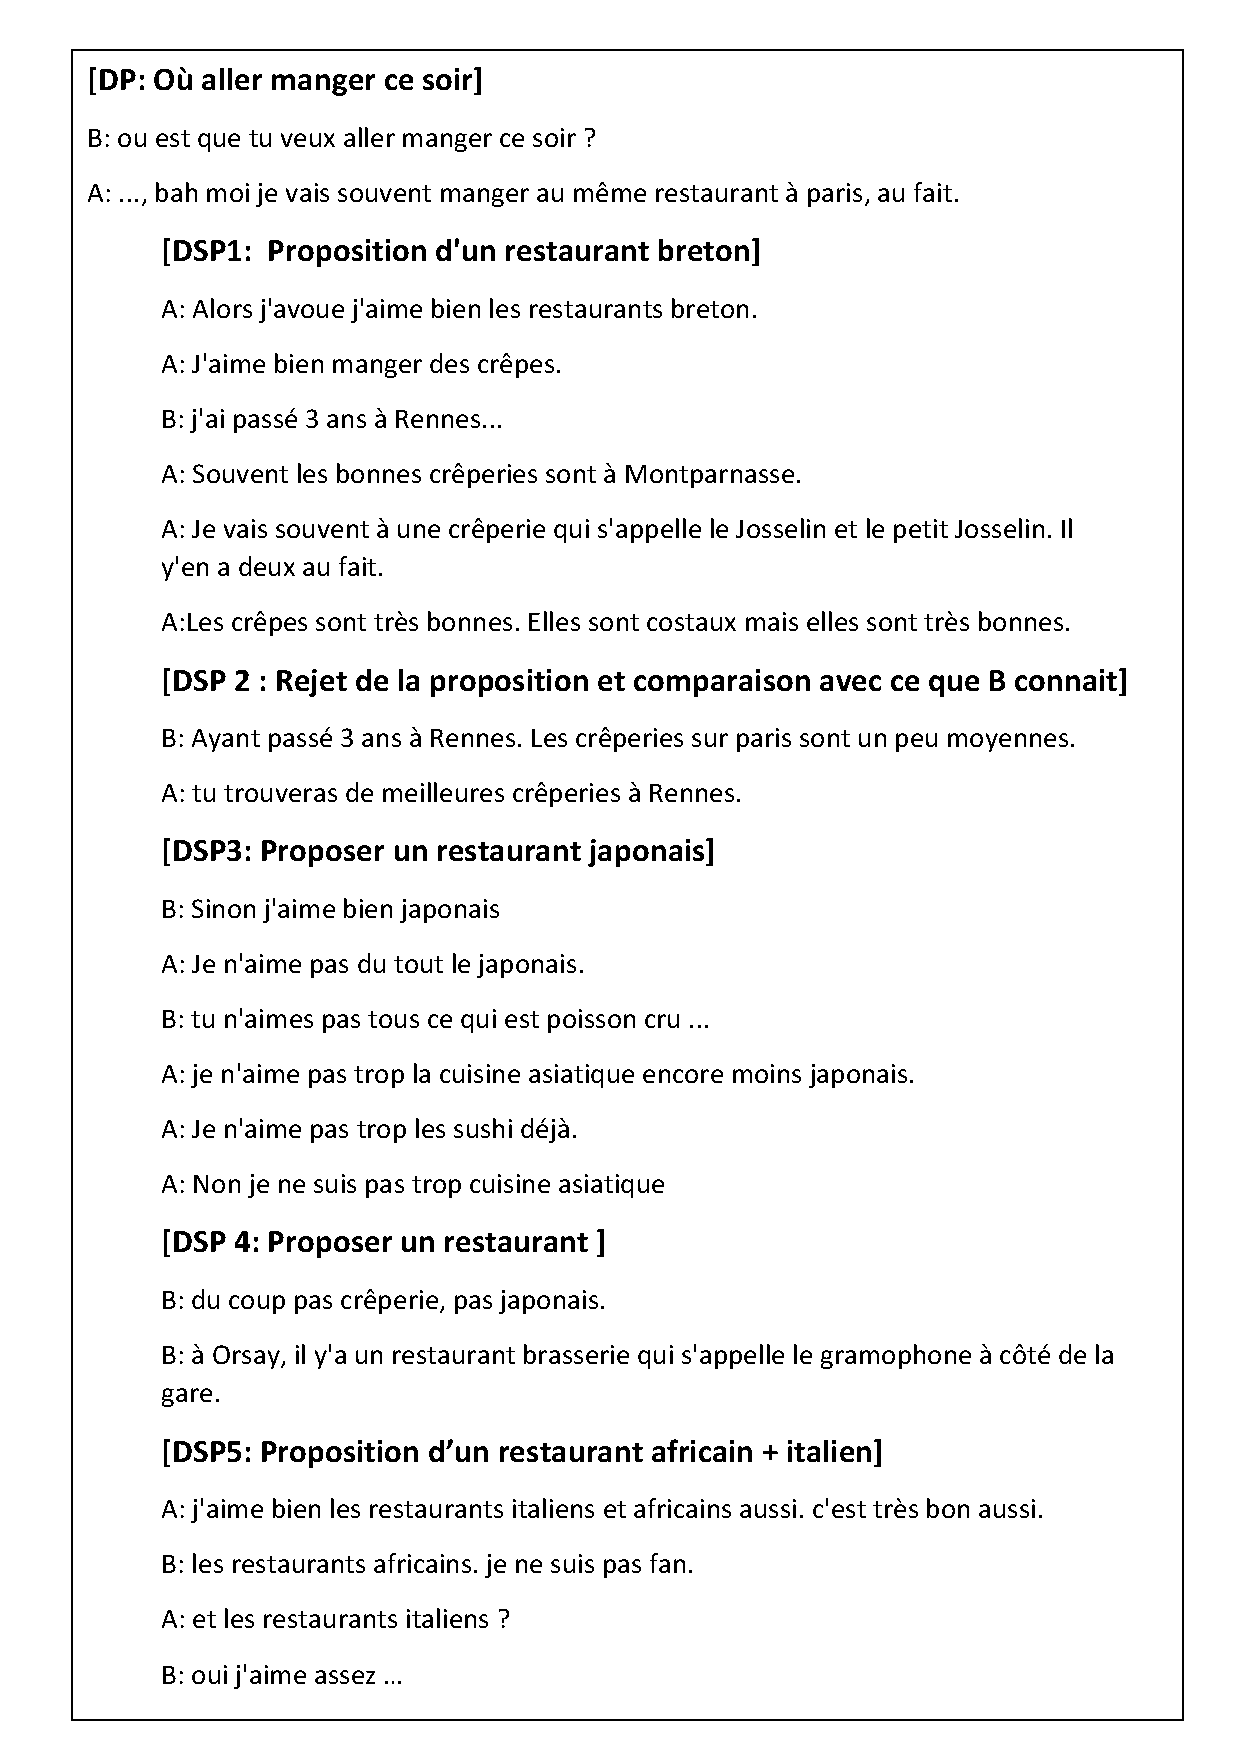
\includegraphics[width=5in]{Figures/dsp_analysis.pdf}
			 	\caption{\label{fig:DSP} Exemple d'une décomposition en \emph{discourse segment} \emph{DS}}
			 \end{figure} 
			 
			 La seconde étape consistait à analyser le but ou l'intention caché derrière chaque \emph{DS}. Par conséquent, nous avons formulé les \emph{DSPs} comme présenté dans l'exemple ci-dessus. L'état attentionnel nous a aidé à la construction des différents \emph{DS} et a formuler les intentions pour chaque \emph{DSP}	
			
			L'analyse du dialogue est présentée dans la figure \ref{fig:DSP}.
			
			
			 
		\subsection{Résultats de l'analyse}
		
			L'analyse en DSPs nous a révélé un nombre de comportements intéressants tant sur l'aspect structurelle de la négociation que sur les stratégies de négociations déployées par les interlocuteurs. 	
			
			Sur l'aspect structurelle, la décomposition du dialogue en \emph{DS} nous a confirmé que les négociateurs s'intéressaient à différents critères pour le choix d'une option (restaurant dans notre exemple). Ces critères sont négociés simultanément durant la négociation jusqu'à ce que les interlocuteurs trouvent un compromis acceptable sur les critères jugés importants. 
			Par exemple, dans le premier dialogue, les interlocuteurs se sont plus intéressés à l'ambiance du restaurant et son emplacement pour le choix final. En revanche, dans le second dialogue, les interlocuteurs se sont principalement concentré sur type et la qualité de la cuisine.
			    
			De plus, Les critères les plus importants sont les premiers à être abordés, et en cas de conflit, d'autre critères sont abordés. 
			Ceci est confirmé par des travaux en négociations automatiques qui mettent en avant l'intérêt de la modalisation multicritères dans les systèmes de négociation \cite{jonker2007agent,lai2004literature}. Ce point sera abordé plus en détails en section suivante. 
			 
			 Nous nous sommes aussi intéressé à l'aspect dialogique de la négociation. En effet, notre modèle se basant sur des actes de dialogue, nous avons analysé les informations échangées lors de la négociation. 
			 Nous avons récolté des informations sur le style linguistique sur lequel seront basés nos actes de dialogues.
			 
			 Finalement, nous avons utilisé la structure attentionnelle et intentionnelle afin d'étudier les stratégies de négociation adoptées par les négociateurs. nous avions analyser la corrélation entre différents comportements durant la négociation influencés par la dimension de la dominance.
			 
			 Le résultats obtenus montrent qu'une relation complémentaire de dominance s'installe entre les négociateurs. C'est à dire que dans la situation où un négociateur prend le pouvoir, l'autre parti accepte cette prise de pouvoir et adapte son comportement.
		
			 La prise de pouvoir se manifeste par les stratégies de prise de parole. Le négociateur avec un haut niveau de dominance avait tendance à prendre la parole plus fréquemment, et plus longtemps. Par exemple, en analysant le \emph{DS1} et \emph{DS3}, nous observons que l'interlocuteur \textit{B} prend plus de tours de parole et pour chaque tour, plusieurs actes dialogiques sont énoncés. 
			 %Par conséquent, en moyenne, la
			 
			 
			 De plus, le style linguistique traduit aussi un comportement de dominance, nous avons observé que la personne dominante avait tendance à facilement exprimer ses préférences (\emph{e.g.} voir \emph{DS3}), argumenter ses choix et décisions dans le but de convaincre l'autre. 
			 
			Ces résultats obtenus ont soutenu les comportements de dominance relayé dans les travaux en psychologie sociale et nous ont aidé à orienter la conception de notre modèle de dialogue
			
		
	
	\section{Domaine de négociation}
	\label{domaine}
	
	%	L'interet d'une négociation multi-critères dans la modélisation d'un sujet social
	% voir intro :https://www.ri.cmu.edu/pub_files/pub4/lai_guoming_2008_1/lai_guoming_2008_1.pdf
	%https://link.springer.com/content/pdf/10.1007/s10458-006-9009-y.pdf
	
		La recherche en négociation automatique peut être divisée en deux catégories en ce qui concerne la représentation du domaine: négociation sur un critère et la négociation multi-critères. Cependant, La littérature existante se concentre plus sur la négociation uni critère \cite{lai2008decentralized,lai2004literature}. 
		
		Dans le cadre d'une interaction avec un négociateur humain, la négociation multi-critère est cruciale. En effet, dans un environnement humain, les négociateurs peuvent discuter de plusieurs critères simultanément, comme nous l'avons vu dans l'étude que nous avions effectué dans la section précédente.  Nous avons observé que les négociateurs s'intéressaient à plusieurs critères pour le choix d'un restaurant. Par exemple le type de cuisine, la location ou encore l'ambiance de ce dernier. Ces critères sont soit abordé simultanément dans la négociation, ou bien un par un. C'est à dire que les négociateurs s'accordaient sur un premier critère avant d'aborder un autre, ou bien discuter des différents critères jusqu'à aboutir a un compromis.
		
		De plus, plusieurs travaux en négociation automatique ont mis en exergue l'apport de la négociation multi-critères. Elle permet d'augmenter la coordination et collaboration durant le processus de négociation afin de rechercher un résultat qui apporte des gains communs pour les deux parties \cite{jonker2007agent,lai2008decentralized,lai2004literature}. \emph{Dedreu} ajoute que la négociation multi-critères offre un contexte pour différents types de stratégies coopératives. D'un coté des négociateurs qui peuvent faire des concessions sur tout les critères. D'un autre coté, des négociateurs qui ont un ordre de priorité sur les critères où ils ont plus tendance à faire des concessions sur les critères avec une priorité faible. 
	
		Les résultats des précédents travaux nous ont motivé à utiliser une représentation multi-critères pour modéliser notre domaine de négociation collaborative. 
		
		\subsection{Représentation formelle des éléments de la négociation}	
		Le but de la négociation est de choisir une \textit{option} $O$ dans l'ensemble des options $\mathcal{O}$ comprenant toutes les options alternatives envisagé pour un sujet de négociation donnée. 
		
		L'évaluation de chaque option repose sur un ensemble de critères $\mathcal{C}$ reflétant les caractéristiques de l'option. Nous définissons l'ensemble $\mathcal{C}$ de $n$ critères, et $C_1,\ldots,C_n$, comme le domaine de valeurs de chaque critère de l'ensemble. 
		Par conséquent, $\mathcal{O}$ peut être défini comme le produit vectoriel de  $C_1\times\ldots\times C_n$ et chaque option $O \in \mathcal{O}$ est un tuple $(v_1,\ldots,v_n)$. 
		
		Par exemple, une négociation collaborative qui porte sur le choix d'un restaurant peut être modélisé en prenant en compte quatre critères à savoir $\mathcal{C}$ = \emph{$\{$Cuisine, Prix, Emplacement, Atmosphère, $\}$}. La table \ref{tab:domain} résume un exemple de domaine de valeurs possible pour chaque critère. Nous faisons l'hypothèse que l'agent connaisse toutes les options pour un domaine donné. Un exemple d'option est  \emph{Anterprima(Italien, coûteux , animé, Montparnasse)}. Au total, $638$ options peuvent être généré à partir du domaine présenté dans la table \ref{tab:domain}. 
		\begin{table}[h]
			\centering
			\begin{tabular}{|p{2.25cm}|p{10cm}|}
				\hline
				Critère $i $ & Domaine de valeur $C_i$ \\
				\hline
				Cuisine & \{Italien, Français, Japonais, Chinois, Mexicain, Turque, Coréen\} \\
				\hline
				Atmosphère & \{Animé, Calme, Romantique, Familial, Cosy, Moderne\} \\
				\hline
				Prix & \{Coûteux, abordable, a prix bas\} \\
				\hline
				Emplacement & \{Père Lachaise, Centre de Paris, Montparnasse, Tour Eiffel, gare du Nord\} \\
				\hline
				
			\end{tabular}
			\caption{Domaine de valeurs pour les critères de choix d'un restaurant} 
			\label{tab:domain}
		\end{table}
		
		
		\subsection{Préférences}
		
			L'agent conversationnel est défini avec un ensemble de préférences formalisé  par un ordre partiel $\prec_i$, défini sur chaque domaine de critères $C_i$. 
					\begin{figure}[] 
						\centering 
						\begin{tabular}{l}
							\subfloat[]{\adjustbox{raise=-5pc}{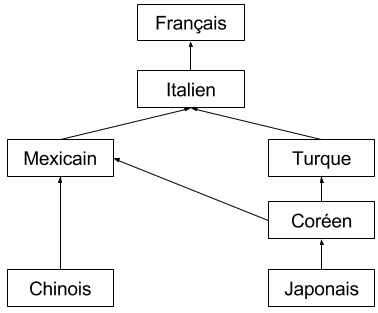
\includegraphics[height=4.8cm]{Figures/cuisine_ex2.png} \label{fig:sub_pref}}}
							\subfloat[]{
								%\input{Figures/Tikz/goldMineState.tex}\label{fig:goldMineState}}  
								\begin{tabular}{|c|c|}
									\hline
									& Critère cuisine \\
									\cline{2-2}
									\parbox[t]{2mm}{\multirow{7}{*}{\rotatebox[origin=c]{90}{\textbf{Préférences}}}} & Japonais $\prec_{cuisine}$ Coréen\\
									\cline{2-2}
									& Chinois $\prec_{cuisine}$ Mexicain\\
									\cline{2-2}
									&  Coréen$\prec_{cuisine}$ Mexicain\\
									\cline{2-2}
									&  Coréen $\prec_{cuisine}$ Turque \\	
									\cline{2-2}
									&  Mexicain$\prec_{cuisine}$ Italien \\
									\cline{2-2}
									&  Turque $\prec_{cuisine}$ Italien\\
									\cline{2-2}
									&  Italien $\prec_{cuisine}$ Français\\	
									\hline								
								\end{tabular}}
							\end{tabular}
							\caption{Exemple de modèle de préférences défini sur le critère cuisine}
							\label{fig:ex_pref}
						\end{figure}
			Nous définissons la relation de préférence comme une relation binaire. Par exemple, $japonais \prec_{cuisine} italien$ signifie que l'agent préfère la cuisine italienne à la cuisine japonaise. Elle est aussi transitive, par exemple, l'agent dispose d'une autre préférence $italien \prec_{cuisine} français$. Nous pouvons donc déduire que l'agent $japonais \prec_{cuisine} français$.
			
			 Ces conditions garantissent que les préférences de l'agent soient cohérentes dans le domaine de la négociation; et la condition de transitivité assure que toutes les valeurs soient comparables. Un exemple de modèle de préférences défini sur le critère de cuisine est présenté dans la figure \ref{fig:ex_pref}.
			
			
			Les préférences étant un aspect essentiel dans la prise de décision durant la négociation, nous avons modélisé une fonction qui représente la valeur d'utilité ou satisfaction pour chaque valeur calculée à partir de l'ensemble des préférences. 
			
			Par conséquent, pour un critère $i\in \mathcal{C}$, pour une valeur $v\in C_i$, l'agent calcule sa \emph{satisfaction} $sat_{self}(v \prec_i)$ pour cette valeur comme le nombre de valeurs qu'il préfère moins dans l'ordre partiel des préférences $\prec_i$. La valeur est ensuite normalisé dans l'intervalle [0,1]:
			
			\begin{equation}
			sat_{self}(v, \prec_i) =	1 - \left( \frac{|\{v' : v' \neq v \  \wedge \ (v \prec_i v')\}| }{( |C_i| - 1 )}\right)
			\end{equation}
			
			La notion de satisfaction est généralisée pour chaque option $ o= (v_1, \ldots, v_n) \in \mathcal{O}$ comme une moyenne des valeurs de satisfactions des différentes valeurs de critères: 
			\footnote{Il existe une grande quantité de travaux  dans le domaine de la prise de décision  qui traitent sur la combinaison de plusieurs critères pour le calcul d'utilité en utilisant par exemple des moyennes pondérées ou des intégrales de Choquet. Nous nous ne intéressons pas dans nos travaux à l'optimisation de la fonction de calcul, pour cette raison nous optons pour une fonction simple d'agrégation de préférences.}
	
			\begin{equation}
			sat_{self}(o, \prec) = \frac{\sum_{i=1}^{n} sat_{self}(v_i, \prec_i) }{n}
			\end{equation}
		
			Un exemple de valeurs de satisfactions calculé à partir de l'ensemble des préférences de l'exemple \ref{fig:ex_pref} est illustré dans la table \ref{tab:sat}
					\begin{table}[h]
						\centering
								{\scriptsize
						\begin{tabular}{ |c|c|c|c|c|c|c|c| }
							\hline				
							valeur & Japonais & Coréen & Chinois &  Mexicain & Turque & Italien & Français \\
							\hline
							
							sat(valeur) & 0.16 & 0.33 & 0.5 & 0.66 & 0.66 & 0.83 & 1\\
							\hline
							
						\end{tabular}}
						\caption{Valeurs de satisfiabilité pour le modèle de préférences défini sur le critère de cuisine}
						\label{tab:sat}
					\end{table}
	
	\subsubsection{Communication}
	\label{sec:communication}
		Le modèle de communication est implémenté sur la plateforme \emph{Disco} \cite{rich09}, qui permet à l'agent de communiquer avec l'utilisateur via des actes de dialogues. Chaque acte de dialogue a un ensemble spécifique d'arguments et est associé à une expression spécifique formulé dans un langage naturel.
		
		La modélisation des actes de dialogue est basée sur les travaux de Sidner \cite{sidner1994artificial} qui avait proposé des actes de dialogues qui permettent à un agent de communiquer dans le contexte de négociation collaborative. Ces actes lui permettent aussi de gérer son état mental en terme d'intentions et croyances communiquées durant la négociation. 
		
		Nous avons définis cinq types d'actes de dialogues génériques et deux actes additionnels pour la gestion de fin de négociation. Les actes de dialogues sont présentés dans la table \ref{table:utt}. Seule la génération en langage naturel (LN) de ces énoncés doit être spécifié pour le domaine de négociation. La valeur /$v$/ dans la table \ref{table:utt} fait référence au format en LN pour exprimer une valeur d'un acte de dialogue.
		Nous utiliserons tout le long de ce manuscrit l'exemple d'une négociation collaborative pour le choix d'un restaurant. 
		
		Chaque type d'acte de dialogue prend un argument qui peut être soit un une valeur de critère  $v \in C_i$, une option $o \in \mathcal{O}$ ou encore critère $i \in \mathcal{C}$. 
		
		En fonction des informations qu'ils communiquent, ces actes de dialogues peuvent être divisé en trois groupes:
		
		\begin{enumerate}
			
			\item \textit{Actes de dialogues informatifs}; ce groupe fait référence aux actes de dialogues utilisés pour échanger des informations sur les préférences respectives des négociateurs, à savoir (\textit{AskValue/AskCriterion} et \textit{StateValue}). 
			Nous avons fait le choix d'attribuer une seule valeur pour les actes informatifs car nous avions observé dans les négociations humain/humain enregistrés que les négociateurs utilisaient généralement une formulation pour exprimer les valeurs qu'ils appréciaient ou non. Par exemple \textit{I (don't)like Chinese restaurants} plutôt qu'une expression avec une comparaison binaire du type \textit{I like Chinese more than French}.
			
			\item \textit{Actes de négociation}; ces actes de dialogues permettent à l'agent de gérer la négociation en exprimant des propositions a son interlocuteur (\textit{Propose}) ou bien de répondre à des propositions exprimées par son interlocuteur. L'agent peut accepter ou rejeter une proposition (\textit{Accept, Reject}). Les valeurs en arguments dans les actes de négociation peuvent être soit des valeurs de critère comme (``Let's go to a Chinese restaurant''), soit des options  (``Let's go to \emph{Chez Francis}''). 
			
			\item \textit{Actes de fin de négociation}; les actes  (\textit{NegotiationSuccess} or \textit{NegotiationFailure}) sont utilisés pour clore une négociation soit par une réussite, soit par un échec. Le choix de l'acte dépend de l'état mental de l'agent. En effet, si une option est acceptée par les deux négociateurs, l'agent exprime alors un \textit{NegotiationSuccess} et termine la négociation. Sinon, si la négociation échoue, alors l'agent exprime un \textit{NegotiationFailure}. Les conditions d'échec d'une négociation sont présentées dans le chapitre suivant. 
			
		\end{enumerate}
		 
		
		
			\begin{table}[t]
					\centering
					\begin{tabular} {|p{3.25cm}|p{6cm}|p{3.25cm}|}
						\hline
						\textbf{Type d'acte de dialogue}  &\textbf{ Génération en NL} & \textbf{Postcondition}\\
						\hline
						StateValue(v) &  I (don't) like /$v$/. \newline  J'aime/Je n'aime pas /$v$/ & Speaker : $v \in S_i$ \newline Hearer:  \newline $v\in A_i$ is likable, $v\in U_i$ otherwise \\
						\hline
						AskValue(v)& Do you like /$v$/ ? & \multirow{2}{*}{} \\
						
						AskCriterion(i) &  What kind of /$i$/ do you like ? & \\
						\hline
						ProposeOption(o)  & Let's go to /$o$/. & $o \in P$\\
						
						ProposeValue(v) & Let's go to a /$v$/. & $v \in P_i$\\
						\hline
						AcceptOption(o)& Okay, let's go to /$o$/.& $o \in T$ \\
						
						AcceptValue(v) & Okay, let's go to a /$v$/.& $v \in T_i$ \\
						\hline
						RejectOption(o) & I'd rather choose  something else. & $o \in R$\\
						
						RejectValue(v) &  I'd rather choose  something else. & $v \in R_i$ \\
						\hline
						NegotiationSuccess &  We reached an agreement. & \multirow{2}{*}{}\\
						\cline{1-2}
						NegotiationFailure &  Sorry, but I no longer want to discuss this. & \\
						\hline
						% Counter Propose & $(r,p)\in C_i^2 \vee (r,p) \in \mathcal{O}^2 $ & I don't want to go to $r$. Let's rather go to $p$ \\
						% \hline 
						% RejectState & $x \in \mathcal{O} \vee x\in C_i$ &  I don't like /$x$/, let's choose something else. \\
						% \hline
						% AcceptPropose & $o \in \mathcal{O}$ & Okay. Let's go to /$o$/.\\
						% \hline
					\end{tabular}
				
				\caption{\label{table:utt}Liste des actes de dialogues pour le modèle de négociation collaborative.}
			\end{table}
		
			\subsection{Mise à jour des connaissances durant la communication}
			
			Le choix d'un type d'acte de dialogue est le résultat d'un processus décisionnel que nous détaillerons dans le chapitre \ref{chap:dec}. 
			Afin de prendre des décisions pertinentes, l'agent garde en mémoire l'historique des échanges d'informations formulées au cours de la négociation.  En effet, après chaque acte de dialogue échangé, l'agent met à jour son état mental.  
			
			
			Pour chaque critère $i\in\mathcal{C}$, l'agent construit un ensemble $S_i \subseteq C_i$ des préférences sur les valeurs de ce critère qu'il a déjà communiqué. Cela prévient la répétition d'informations échangées précédemment. 
			De plus, l'agent garde en mémoire les préférences communiquées par son interlocuteur. Nous notons les ensembles $A_i\subseteq C_i$ et $U_i\subseteq C_i$, respectivement l'ensemble des valeurs que l'interlocuteur a communiqué comme appréciées (\textit{I like $\ldots$}) et non appréciées  (\textit{I don't like $\ldots$}) à travers l'acte de dialogue \textit{StatePreference}. 
			
			L'agent maintient aussi des informations sur le cours de la négociation. Soient $P_i \subseteq C_i$, $T_i\subseteq C_i$ et $R_i\subseteq C_i$ les ensembles de toutes les valeurs proposées, acceptées et rejetées pour chaque type de critère. 
			De même, nous considérons $P\subseteq \mathcal{O}$, $T\subseteq \mathcal{O}$ et $R\subseteq \mathcal{O}$ les ensembles de toutes les options proposées, acceptées et rejetées au cours de la négociation.
			
			\subsubsection{Préférences de  l'interlocuteur}
				Dans le contexte d'une négociation collaborative, l'agent prend en compte les préférences de son interlocuteur pour prendre des décisions. Pour cette raison, l'agent a besoin de collecter des informations sur les préférences de son interlocuteur. En effet, l'agent utilise les ensembles $A_i$ et $U_i$ qui représentent les préférences de l'interlocuteurs collectés lors des interactions, pour calculer une valeur de \emph{satisfaction}  qu'a l'interlocuteur pour toute valeur $v\in C_i$: 
				
					\begin{equation}
					sat_{other}(v)= \left\{\begin{array}{ll}
					1	 & \mathrm{if\ }  c \in A_i\\
					0    & \mathrm{if\ }c \in U_i\\
					0.5	 & \mathrm{otherwise}
					\end{array}\right.
					\end{equation}
					
				Notons que l'agent possède une connaissance partielle des préférences de son interlocuteur. Par conséquent, les préférences sur certaines valeurs peuvent rester inconnues. Dans  le contexte d'une négociation collaborative, ces valeurs sont considérées comme \textit{potentiellement satisfiables}. Par conséquent, nous leur affectons une valeur arbitraire fixée à \textbf{0.5}.
				
	\section{Conclusion}
			Ce chapitre a présenté les différents éléments de notre modèle de négociation collaborative essentiels pour étudier l'impact de la dominance durant la négociation. Nous avons fait le choix de construire un modèle de négociation générique capable de gérer différent sujets de conversation. De plus, nous avions l'objectif de définir un domaine qui nous permettrait de refléter différents comportements durant la négociation. 
			
			Premièrement, nous avons appuyé notre recherche par une collecte de données où nous avons enregistré des négociations humains/humain qui nous a révélé nombres de comportements qui apparaissent au cours de la négociation. Ces résultats ont été discutés et nous ont permis de guider notre recherche. Entre autres, les résultats obtenus nous ont soutenu dans notre choix de modéliser une négociation  multi-critères.
			Nous avons donc présenté le domaine de négociation multi-critères ainsi que la représentation classique de préférences.
			
			Nous avons ensuite présenté notre modèle de communication. Le modèle proposé permet à l'agent de mener une négociation collaborative. En effet, les actes proposées permettent à l'agent d'une part d'échanger des informations sur les préférences et d'autre part de négocier. 
			
			Ce modèle de négociation collaborative présente une base solide pour construire un modèle de décision qui prend en compte les comportements de dominance. Le chapitre suivant présente donc la construction du modèle décisionnel de notre système de négociation. Nous présenterons un algorithme décisionnel capable de refléter différentes stratégies de négociation en fonction de la position de dominance de l'agent dans l'interaction.
					
			
%	Présentation des actes de dialogues avec leurs catégories et conditions d'applicabilité. 
%	\textcolor{red}{Expliquer que note choix d'utterances se basent sur les travaux de Candece Sidner. De plus, l'analyse en DSP nous a révélé que les participants utiliser des doubles utterances dans leur négociation, et ceci de manière réccurente. Ceci traduisait de plus leur stratégies de négociation influncé par des comportements de pouvoir}
	

%%%%%	
	\label{chap:dec}
	%Après avoir défini la relation interpersonnelle de dominance dans le chapitre \ref{chap:etat}, ainsi que sa manifestation dans l'interaction tant sur l'aspect verbal que non verbal, nous avons ensuite détaillé son impact sur les stratégies de négociations. 
	
	Ce chapitre introduit le modèle de décision d'un agent négociateur qui lui permet d'adapter sa stratégie de négociation à la relation de dominance qu'il vise à instaurer avec son interlocuteur. Dans la section 1, nous définissons les principes de décisions basés sur les comportements de pouvoir inspirés des travaux en psychologie sociale. Dans la section 2, nous présentons un premier modèle décisionnel utilisant des règles de décisions.  Pour ce modèle, nous nous sommes basés sur la structure d'arbres défini dans \emph{DISCO} \cite{rich09} et nous discuterons ses limites. Ensuite dans la section 3, nous présenterons notre modèle décisionnel final qui prends en compte les comportements de dominance de l'agent associés à ses préférences pour construire sa stratégie de négociation. Ensuite, nous présenterons deux études visant à valider le modèle décisionnel dans les deux cas d'interaction agent/agent et agent/humain.
	
	\section{Comportements de pouvoir et stratégies de négociation}
	\label{chap:domer}
	Comme nous l'avons présenté dans le chapitre \ref{chap:etat}, nous nous sommes essentiellement basés sur les travaux en psychologie sociale pour la définition de la dominance. 
	La dominance comme relation interpersonnelle est présentée comme la capacité à exprimer des comportements verbaux et non verbaux par lesquels  l'influence est atteinte. Prenant cette définition comme point de départ, nous nous sommes ensuite intéressé à la manifestation des comportements de dominance durant le processus de négociation et comment ces comportements influençaient les stratégies de négociations dans le contexte d'interaction humain/humain. 
	
	Dans ce qui suit, nous présentons \emph{trois principes} de comportements extraits des travaux en psychologie sociale qui ont étudiaient l'impact du pouvoir sur les négociateurs et leur stratégies.
	
	\begin{enumerate}
		\item \textbf{Niveau d'exigence et de concessions:} Les négociateurs dominants affichent un niveau d'exigence plus important comparés aux négociateurs soumis. Par ailleurs, les exigences des négociateurs soumis diminuent avec le temps. Ceci se traduit par des concessions plus importantes comparés aux négociateurs plus dominants. \cite{de1995impact}
		
		\item \textbf{Soi \emph{vs} autrui:} Les négociateurs soumis prennent en compte les préférences de leur interlocuteur dans la négociation, tandis que les négociateurs  dominants sont centrés sur eux-mêmes et s'intéressent uniquement à la satisfaction leurs propres préférences. \cite{fiske1993controlling,de1995impact}
		
		\item \textbf{Contrôle du flux de la négociation:}
		Les négociateurs dominant ont tendance à faire le premier pas et à prendre les devants dans la négociation \cite {magee2007domer}. Ils sont centrés sur l'avancement du processus de prise de décision, en prenant des décisions rapides \cite{zablotskaya2012relating}.
		A l'opposé, les négociateurs moins dominants visent à construire un modèle précis des préférences du partenaire de négociation. 
		Par conséquent,  ils posent plus de questions afin de collecter les informations nécessaires qui leurs permettent de prendre la décision la plus équitable(\emph{e.g}  faire des propositions)~\cite{de2004influence}. 
		
	\end{enumerate}
	
	
	Le but est de construire un modèle de décision capable d'illustrer ces comportements de dominance et par conséquent, adapter la stratégie de négociation en fonction de la dominance de l'agent.
	
	Dans ce qui suit nous présenterons le modèle décision de l'agent qui prend en compte la relation de pouvoir.
	
	
	\section{Règles de décision}
	Dans le cadre de cette thèse, nous avons construit un premier modèle de décisions composé de règles de décision modélisées sous forme d'arbres de dialogues. L'implémentation de notre système de dialogue est géré par le logiciel \emph{Disco}. Disco est une implémentation d'un ``collaborative discourse manager'' inspiré d'une théorie de dialogue collaboratif comme \emph{Collagen} \cite{rich1997collagen}. Disco est un système qui permet la génération de dialogues orienté tâches pour lequel il utilise le formalisme des \textbf{HTNs} (Hierarchical Task Networks) \cite{erol1994htn} pour la gestion des tâches. Il est implémenté avec le standard ANSI/CEA-2018 : chaque tâche est définit avec des préconditions, des effets et des postconditions. Les tâches sont regroupées par \emph{recettes} munies de conditions d'applicabilité.
	
	De plus, \emph{Disco} a été étendu avec un module génération d'arbres de dialogues afin de communiquer et collaborer avec l'utilisateur pour la réalisation des tâches. Ce module est nommé Disco for Games (D4g) et permet de définir des sémantiques d'actes de dialogue. D4g est déjà fourni avec un ensemble d'actes de dialogue.
	
	Nous avons complété ce système avec les actes de dialogues présenté dans la section \ref{sec:communication} afin qu'il puisse supporter la négociation sur les préférences.
	
	Pour chaque acte de dialogue que l'agent reçois, nous modélisons l'ensemble des réponses que l'agent peut sélectionner. Par exemple, suite à un acte \emph{Propose} énoncé par l'utilisateur, l'agent peut répondre par un \emph{Accept}, un \emph{Reject} ou un autre \emph{Propose}. Par exemple:
	("User: Je propose que nous allions dans un restaurant Chinois. 
	
	Agent: je propose que nous allions plutôt dans un restaurant Japonais"). 
	
	Chaque branche est définie avec des conditions d'applicabilités pour décider quelle réponse est adoptée. 
	Ces conditions prennent en compte la dominance de l'agent en plus du contexte courent de la négociation. Dans l'exemple précédent, l'agent doit être dominant pour répondre à un Propose par un autre Propose. 
	
	
	\subsection{Sélection de l'acte de dialogue}
	Nous avons initialisé l'agent avec un comportement de pouvoir parmi trois types de comportements de pouvoir inspirés de la littérature en psychologies social.  L'agent peut suivre un comportement \emph{dominant, soumis} ou \emph{neutre}. 
	
	En fonction de l'acte de dialogue que l'agent reçoit, nous générons un ensemble de réponses possibles. Chaque réponse dépend du pouvoir de l'agent. Le système de dialogue offre à l'utilisateur la liberté de choisir n'importe quel acte de dialogue pour son tour de parole. Disco déroule alors l'arbre de dialogue correspondant de gauche à droite (en commençant par la branche la plus à gauche). La première branche applicable rencontrée est directement exécutée sans vérifier les branches restantes.
	
	Notons que dans la suite, chaque arbre de dialogue est défini avec une condition de sortie qui clos la négociation avec un échec. Cette dernière est activée seulement par agent \emph{dominant} dans la situation où toutes les valeurs restantes ne sont pas acceptables. 
	
	\subsubsection{AskPreference}
	A la réception d'un \emph{AskPreference}, l'agent répond en exprimant ses préférences sur la question demandée comme présenté dans la figure .. .
	
	\subsubsection{State Preference}
	Le comportement standard qu'un agent adopte à la réception d'un \emph{StatePreference(v)} est de donner son opinion sur la valeur exprimée (c-à-d que l'agent calcule la valeur de satisfiabilité de \textit{v}). Cependant, si l'agent a déjà exprimé ses préférences sur ces valeurs, il va vouloir choisir un autre acte de dialogue en fonction de la relation sociale:
	\begin{itemize}
		\item \emph{Propose(x)}: Si la valeur exprimée par l'utilisateur est acceptable (voir figure \ref{pseudo}) pour l'agent, il va proposer de choisir cette valeur. Ce comportement relate le principe 1.
		\item \emph{Propose}: Si le nombre de \emph{StatePreferences} autorisé est atteint (voir figure \ref{alg:maxtours}), l'agent doit respecter le principe 3 et faire évoluer la négociation. La valeur proposée doit respecter les préférences de l'agent. 
		\item \emph{StatePreference}: l'agent est \emph{neutre}, il va vouloir exprimer ses préférences afin de construire une meilleure connaissance.
		\item \emph{AskPreference}: l'agent est \emph{soumis}. Dans le cas où toutes les valeurs du critères courent ont été discutés, l'agent va respecter le principe 3 et faire évoluer la négociation en ouvrant la discussion sur un autre critère.
	\end{itemize}
	
	\begin{figure}[]
		\begin{algorithmic}[1]\small
			\Function{MaxStatements}{}
			\State $nbTours$ = Nombre de \emph{StatePreferences} exprimés successivement.
			\State $maxTours$ 
			\If{($dominant$)} 
			\State $maxTours = 1$
			\EndIf
			\If{($peer$)} \State $maxTours = 2$
			\EndIf
			\If{($soumis$)} 
			\State $maxTours = 4$
			\EndIf
			\State $retrun$ $nbTours\geq maxTours$
			\EndFunction
		\end{algorithmic}
		\vskip 8pt
		\label{alg:maxtours}
		\caption{Maximum de tours de \emph{StatePreference} autorisé en fonction du pouvoir de l'agent}
	\end{figure} 
	\subsubsection{Propose}
	A la réception d'un \emph{Propose} comme présenté dans la figure ..., l'agent choisit sa réponse en fonction de l'\emph{acceptabilité} de la proposition.
	Nous avons écrit l'algorithme d'acceptabilité afin qu'il s'adapte à la valeur de pouvoir de l'agent. Ce choix permet de refléter les comportements du principe 2 \emph{niveau d'exigences et concessions}.
	
	En effet, au fur et à mesure que la négociation évolue, l'agent va faire des concessions sur certains critères. Par exemple, il peut considérer que le critère de \emph{localisation} n'est plus important pour le choix d'un restaurant. Par conséquent, il considérera que toute valeur de \emph{localisation} est désormais \emph{acceptable}.
	
	Par ailleurs, la notion d'exigence apparaît dans l'algorithme ci-dessous. Si l'agent est \emph{dominant}, l'ensemble de valeurs acceptables est plus restreint qu'un agent \emph{soumis}.
	
	\begin{figure}[]
		\begin{algorithmic}[1]\small
			\Function{isAcceptable}{$proposal$}
			\If{(type de $proposal$ n'est pas un critère important)} 
			\State return $true$
			\EndIf
			
			\State List = trier les valeurs par ordre décroissant de préférences
			\If{($dominant$)} 
			\State $return$ index($proposal$)< $size(List)/2$
			\EndIf
			\If{($soumis$)} 
			\State return $return$ index($proposal$)< $size(List)/4$
			\EndIf
			\EndFunction
		\end{algorithmic}
		\vskip 8pt
		\label{pseudo}
		\caption{Calcul d'acceptabilité d'une proposition $value$}
	\end{figure} 
	
	
	L'arbre de décision produit pour répondre à un \emph{Propose(p)} est présenté dans la figure .... 
	\begin{itemize}
		
		\item  \emph{Accept(p)}: Si la proposition \emph{p} est acceptable, l'agent doit exprimer un \emph{Accept(p)}. Sinon, l'agent doit faire évoluer la négociation pour trouver un meilleurs compromis. En fonction de la relation de pouvoir l'agent choisit un acte de dialogue spécifique.
		\item \emph{Ask :} l'agent \emph{soumis} va suivre les comportements décrit dans les principes 1 et 3. En effet, il va essayer de collecter plus de connaissances sur les préférences de l'autre et ainsi prendre en compte ses préférences. De plus, en vue du principe 2 qui affirme qu'un agent soumis doit faire des concessions, l'agent soumis n'est pas autorisé à exprimer plus d'un nombre de rejets successifs.  
		\item \emph{Reject :} l'agent qui n'est pas dominant (\emph{i.e. soumis ou neutre}) rejete une proposition qui n'est pas acceptable.
		\item \emph{Propose :} suivant le principe 3, l'agent \emph{dominant} fait évoluer la négociation en proposant une autre valeur qui respecte mieux ses préférences. 
	\end{itemize}
	
	
	
	\subsubsection{Accept }
	A la réception	d'un \emph{Accept}, nous séparons deux cas de réponses en fonction du type de la valeur acceptée $v$.
	Premièrement, $ v \in \mathcal{O}$ une \textit{option}, l'agent clos la négociation par un \emph{succès}.
	Sinon, $v \in C_i$ est une valeur de critère, l'agent entame la négociation sur un autre critère et sa réponse sera choisie en fonction de la relation de pouvoir à exprimer.
	
	\begin{itemize}
		\item \emph{Propose}: La condition d'applicabilité pour cet acte de dialogue dépend du pouvoir de l'agent. Un agent \emph{dominant} entamera la négociation sur le nouveau critère en proposant une valeur qui respecte ses préférences. Cependant, un agent \emph{soumis} n'est autorisé à faire une proposition que s'il a des connaissances sur les préférences de l'autres,  communiqués par des \emph{StatePreferences}, qui lui permettront de prendre une décision équitable. cet algorithme traduit les comportements présentés dans les principes 1 et 3. 
		
		\item \emph{AskPreference}: Comme présenté dans le principe 3, l'agent est \emph{soumis} collecte le plus d'informations possibles sur les préférences de son interlocuteur. 
		\item \emph{StatePreference}: L'agent est \emph{neutre} ouvre la négociation en communiquant ses préférences sur le nouveau critère à discuter. 
		
	\end{itemize}
	
	%				\begin{figure}[]
	%					\begin{algorithmic}[1]\small
	%						\Function{CanPropose}{}
	%						\If{($dominant$)} 
	%						\State return $true$
	%						\EndIf
	%						
	%						\State 
	%						\If{($soumis$)} 
	%						\State l'agent a des connaissances suffisantes sur les préférences de l'interlocuteur
	%						\State return $true$
	%						\EndIf
	%						\EndFunction
	%					\end{algorithmic}
	%					\vskip 8pt
	%					\label{alg:canPropose}
	%					\caption{Calcul d'acceptabilité d'une proposition $value$}
	%				\end{figure}
	%				
	
	\subsubsection{Reject}
	Suite à un \emph{Reject}, l'agent choisis une réponse en suivant les trois principes comme présenté ci-dessous:
	\begin{itemize}
		\item \emph{AskPreference}: Si la proposition d'un agent \emph{soumis} est rejetée, il va considérer qu'il n'avait pas assez de connaissances pour prendre une bonne décision. Pour compenser, il va demander à l'utilisateur ses préférences sur des valeurs qu'il ne connaît pas déjà. 
		
		\item \emph{Propose}: Suivant les principes 1 et 3, l'agent \emph{dominant} fait avancer la négociation en proposant de nouvelles valeurs. Cependant, si la valeur rejetée se trouve être la valeur qu'il préfère le plus, il va refuser de concéder et donc proposer la valeur encore une fois. Ce comportement est fidèle au principe 2. 
		
		\item \emph{StatePreference}: l'agent \emph{peer} continue la négociation en exprimant ses préférences sur d'autres valeurs. 
	\end{itemize}	
	%----------------------------------------------------------------
	
	\subsubsection{Exemple}
	Nous présentons un dialogue généré en utilisant notre modèle de dialogue. Deux agents\textit{A} et \textit{B}
	
	
	A: "Let's go to a Chinese restaurant."
	
	B: "I like Italian more than Chinese restaurants."
	
	A: "Let's go to a quiet restaurant."
	
	B: "I don't like quiet restaurants."
	
	A: "Let's go to a cheap restaurant."
	
	B: "Do you like quiet or lively restaurants? "
	
	A: "I like quiet restaurants."
	
	B: "I like lively restaurants."
	
	A: "Let's go to the Samura restaurant. It's a lively, cheap Japanese restaurant."
	
	B: "What kind of cuisine do you like?"
	
	A: "I like Chinese restaurants."
	
	B: "I like Italian restaurants."
	
	A: "Let's go to the Dragon restaurant. It's a lively, cheap Chinese restaurant."
	
	B: "Okay. Let's go to the Dragon restaurant."
	
	A: "Okay. I'll call to book a table."
	
	
	\subsection{Evaluation du modèle}
	\subsection{Limites des arbres de dialogue}
	Parler de l'étude qui a montré une ambiguïté dans la perception des comportement et la capacité à isoler l'impact de chaque principe sur la prise de décision
	
	Comportement incongrue ou non attendue.
	
	Situation de \textit{breakdown}, du a une modélisation manuelle, nous avions rencontrer des situations où aucune condition d'applicabilité n'étaient vrai. 
	
	Pour toutes ces raisons, nous avons repenser notre solution pour qu'elle soit plus fidèle aux principe de négociation et qu'elle puisse refléter les comportements de pouvoir. 
	
	\section{Modèle de décision basé sur les comportements de pouvoirs}
	
	Nous proposons un modèle computationnel de décision, qui reprend les trois principes de pouvoir dans le modèle décisionnel de l'agent. 
	A cause de la rigidité des arbres de dialogues, nous adaptons la solution afin qu'elle soit plus flexible de l'utilisateur et surtout afin que les comportements de pouvoir soient plus saillant dans les décisions de l'agent.
	
	Par conséquent, nous présentons dans ce qui suit, l'adaptation algorithmique de chaque principe de dominance extraits de la psychologie sociale.
	
	L'agent est défini avec une valeur de dominance $dom \in [0,1]$ qui représente sa position de dominance dans l'interaction, tel que plus $dom$ se rapproche de 1, plus l'agent est dominant. 
	
	\subsection{Principe 1: Niveau d'exigence}
	
	Selon notre premier principe, le niveau d'exigence devrait être plus important chez les agents dominants. Cependant, au cours d'une négociation collaborative, les deux négociateurs sont amenés à réduire leur niveau d'exigences parce qu'ils veulent parvenir à un accord. Les psychologues observent des concessions plus importantes pour les négociateurs soumis. 
	
	Nous avons implémentés ces comportements en deux phases. En effet, afin de modéliser la différence d'exigence dans la négociation, nous avons implémenté une fonction de satisfiabilité qui prend en compte la valeur de pouvoir initiale de l'agent. 
	
	Soit $S$ l'ensemble de valeurs satisfiables pour l'agent. Ceci se traduit par les valeurs que l'agent se dit \textit{"aimer" (i.e. l'expression d'un } \emph{StatePreference}). Cet ensemble varie en fonction de la valeur $dom$ de l'agent:
	
	\begin{equation}
	\forall v,\hspace{2mm} v\in S\hspace{2mm}\mathrm{iff}\hspace{2mm}sat(v) \geq dom
	\end{equation}
	
	En effet, une valeur est dite \textit{satisfiable} si sa valeur de satisfiabilité est plus grande que la valeur de dominance de l'agent.
	
	Par exemple, pour le même ensemble de valeurs présentés dans l'exemple présenté dans le table \ref{tab:sat} et les mêmes relations de préférences, deux agents avec des valeurs de dominance différentes n'ont pas le même niveau d'exigence. Supposons, un agent$_A$ dont la dominance est à $dom_A=0.7$ et un autre agent$_B$ dont la dominance est à $dom_B=0.4$, pour le même ensemble de préférences ( voir table \ref{tab:sat} ), les deux agents ont un ensemble de valeurs satisfiables différents comme présenté dans la table \ref{tab:exSat}.
	
	\begin{table}[h]
		\centering
		{\scriptsize
			\begin{tabular}{ |c|c| }
				\hline
				\textbf{Agent} & \textbf{valeurs satisfiables} \\
				\hline				
				$S_A$ & Italien , Français \\
				\hline
				
				$S_B$ & Chinois ,  Mexicain , Turque , Italien , Français\\
				\hline
				
			\end{tabular}}
			\caption{Ensemble de valeurs satisfiables de l'agent$_A$ et l'agent $_B$}
			\label{tab:exSat}
		\end{table}
			\begin{floatingfigure}[l]{2.1 in}
				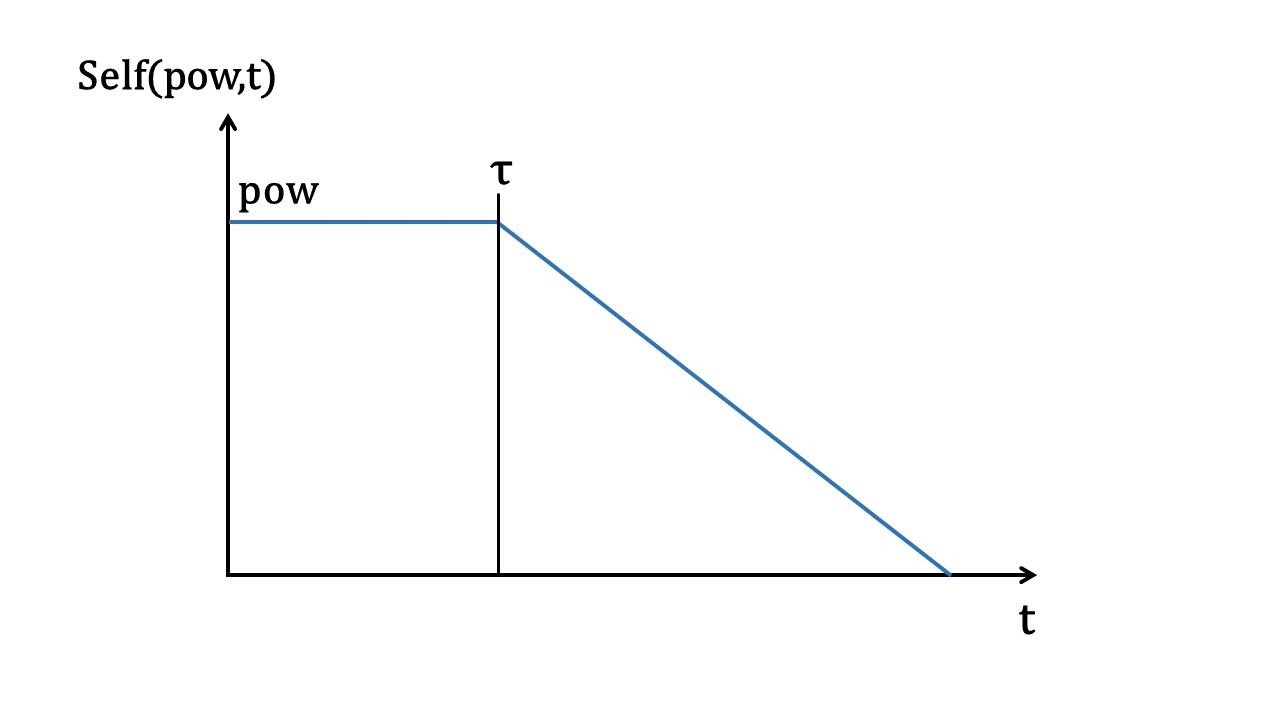
\includegraphics[width=2in]{Figures/sv3.png}
				\caption{\label{fig:conc}Courbe de concession reprenant le principe 1}
			\end{floatingfigure} 
			
	
	
	Concernant, les comportements de concession, nous avons élaboré une \emph {courbe de concession} illustrée sur la figure \ref{fig:conc}. 
	

	Soit $ self (dom, t) $ une fonction variant dans le temps, suivant la courbe de concession:
	\begin{equation}
	self(dom, t) = \left\{\begin{array}{ll}
	dom & \mathrm{if\ } (t \leq \tau)\\
	max(0, dom - (\frac{\delta}{dom} \cdot (t - \tau))) & \mathrm{otherwise}
	\end{array}\right.
	\end{equation}
	
	
	
	tel que :
	\begin{itemize}
		\item $t \geq 0$ est le nombre de propositions ouvertes ou rejetées ayant été exprimé durant la négociation.
		\item $\tau > 0$ le nombre minimal de propositions pour que les concessions commencent.
		\item  $\delta > 0$ un paramètre de calcul de la courbe de concession.
		
	\end{itemize}  
	
	La fonction $self(dom,t)$ représente le poids que l'agent attribut à sa satisfaction personnelle par rapport à la satisfaction de son partenaire de négociation. Plus la dominance de l'agent est élevée, plus son niveau d'exigence est important. Par ailleurs, la courbe de concession décroît plus rapidement pour des valeurs de dominance faibles.
	
	Ces comportements d'exigences et de concessions sont modélisés pour calculer l'acceptabilité d'une proposition 
	
	L'acceptabilité d'une valeur de critère $v \in C_i$ est défini comme une fonction booléenne:
	\begin{equation}
	\vspace{-.5em} 
	acc(dom,v, t) = sat_{self}(v, \prec_i) \geq  (\beta \cdot self(dom,t))
	\end{equation}
	
	\medskip
	où $\beta>0$ est un paramètre théorique qui définit le poids accordé au niveau d'exigence.
	
	cette fonction est généralisable aux options $o \in O$: $acc(dom,o, t) = sat_{self}(o, \prec) \geq  (\beta \cdot self(dom,t))$. Elle est utilisée afin de déterminer si une proposition est acceptable.
	
	
	
	
	\subsection {Prise en compte des préférences de soi Vs autrui}
	Selon notre second principe, les négociateurs dominants donnent plus de poids à leur propre satisfaction qu'a leur partenaires de négociation. 
	Pour implémenter ce principe dans le contexte de la négociation collaborative, nous calculons dans quelle mesure une proposition donnée est \emph{tolérable} pour la satisfiabilité de l'agent et de son partenaire.
	En effet, à chaque fois que l'agent énoncera une proposition, la valeur de cette dernière doit prendre en compte les préférences des deux interlocuteurs. 
	Donc, pour chaque critère $i\in\mathcal{C}$, considérons le sous ensemble $V_i\subseteq C_i$ de valeurs acceptables pour l'agent:

	\begin{equation}
	V_i(dom,t) = \{ v\in C_i : acc(dom,v,t) \}
	\end{equation}
	
	Cet ensemble correspond à toutes les propositions acceptables qu'un agent pourrait faire à un moment donné de la négociation.
	
	Nous calculons la tolérabilité d'une valeur donnée $ v \ dans V_i (dom, t) $ en équilibrant entre les préférences de l'agent et celles de son partenaire. Nous supposons que l'agent donne un poids à la satisfaction de son partenaire qui est complémentaire à son auto-satisfaction:
	
	\begin{equation}
	\begin{split}
	tol(v, t, \prec_i, A_i, U_i, dom) & = self(dom, t)  \cdot sat_{self}(v, \prec_i) \\
	& +  (1 - self(dom, t)) \cdot sat_{other}(v, A_i, U_i)
	\end{split} 
	\end{equation}
	

	Nous généralisons cette fonction à toute option $o=(v_1,\ldots,v_n) \in O$:
	
	\begin{equation}
	tol(o, t, \prec, A, U, dom) = \frac{ \sum_{i}^{n} tol(v_i, t, \prec_i, A_i, U_i, dom) } {n}
	\end{equation}
	
	\noindent
	Par conséquent, l'agent propose la valeur la plus \emph{tolérable} dans l'ensemble $V_i$:
	\begin{equation}
	propose(V_i, \prec_i,dom) =  \operatorname*{arg\,max}_{v \in V_i} ( tol(v))
	\end{equation}
	
	Par conséquent, plus l'agent est soumis, plus il va considérer les préférences de son interlocuteur.
	
	\subsubsection*{Résumé des paramètres computationnels}
	\begin{itemize}[noitemsep]
		
		\item $\pi \in $[0,1] : La frontière entre  les comportements soumis et dominants utilisé dans le choix d'un type d'acte de dialogue. (voir )
		\item $\tau > 0$ : le nombre minimal de propositions ouvertes ou rejetées avant le début de la concession.
		\item $\delta > 0$ : paramètre dans la pente de la courbe de concession.
		\item $\alpha> 0$: Le nombre maximums d'actes de dialogues informatifs consécutifs.
	\end{itemize}
	
	\subsection{Contrôle de la négociation}
	
	Le troisième principe stipule que les négociateurs dominants ont tendance à contrôler la négociation.
	Nous avons implémenté ce principe à travers un algorithme pour le choix de l'acte de dialogue à énoncer, comme présenté dans la table \ref{table:uttChoice}.
	
	Nous avons défini un seuil $\pi$  qui divise le spectre de dominance en deux, à savoir comportements dominant, où soumis.
	
	Prenant en compte trois paramètres; la valeur de dominance $dom$, l'acte de dialogue énoncé par le partenaire $u^{-1}$ et l'état courent de la négociation, l'agent sélectionne le premier acte dans la table \ref{table:uttChoice} dont la condition d'applicabilité est vérifiée.  
	
	
	Par exemple, un agent dominant mettra fin à la négociation dès que toutes les options restantes seront inacceptables (ligne 2). Un agent soumis rejettera et exprimera une \emph{State}, afin de justifier son refus et expliquer pourquoi la proposition n'est pas acceptable (ligne 14). S'il n'y a pas de proposition ouverte, l'agent avec un pouvoir faible demandera de nouvelles informations (ligne 18 -19).
	
	Dans notre modèle, un agent peut exprimer plusieurs actes de dialogues dans un même tour de parole. Ces cas sont représentés avec un signe $"+"$ dans la table \ref{table:uttChoice}.
	
	En fonction de la valeur de dominance, l'agent va adopter différentes stratégies dans la sélection de l'acte de dialogue à exprimer. En effet, dans les travaux en psychologie social, les négociateurs dominants se concentrent sur l'avancement de la tâche de négociation. Ceci ce traduit par le choix d'actes de négociations (ProposeValue /ProposeOption, RejectValue /RejectOption, AcceptValue/ AcceptOption) comme il est présenté dans les lignes (4 à 10).
	
	L'agent priorise les actes de négociations plutôt que les actes d'échanger d'informations sur les préférences. En effet, comme présenté à la ligne 3, après un nombre de tours $ \alpha $ consacrés au partage d'informations, l'agent fera plutôt des propositions que informer le partenaire de ses goûts. Un exemple est présenté dans le dialogue \ref{fig: ex-dialogue}.
	
	Au contraire, un négociateur soumis se concentrera sur la construction d'un modèle précis des préférences de son partenaire afin de prendre la décision la plus équitable. Il se concentrera plus sur \emph {actes d'échanges d'information} (StateValue ou AskValue / AskCriterion) comme le montre les lignes (18-20). De plus, les mouvements de négociation sont limités par des conditions qui garantissent que l'agent ait rassemblé suffisamment d'informations sur les préférences de son partenaire avant d'exprimer une proposition (ligne 16-17).
	
	\begin{table}[!t]
		
		\centering
		\begin{tabular}{|p{.5cm}|p{.9cm}|p{4cm}|p{7.5cm}|}
			\hline
			\parbox[t]{3mm}{\multirow{5}{*}{\rotatebox[origin=c]{90}{\centering \textbf{dom  $>\pi$}}}}&$N $de ligne& \textbf{Acte de dialogue} & \textbf{Condition} \\
			\cline{2-4}
			&1&NegotiationSuccess & $\exists o \in T\cup P$, $acc(dom,o,t)$ \\
			\cline{2-4}
			& 2& NegotiationFailure & $ \forall o \in \mathcal{O},  \neg acc(dom,o,t)$\\
			\cline{2-4}
			&3& StateValue(v) & $type(u^{-1}) = AskPreference \land n < \alpha$ \newline $n$ est le nombre d'actes informatifs successifs\\
			\cline{2-4}
			&4& AcceptValue(v)+ \newline ProposeValue(c) & $ \exists v \in P_i$ / $acc(dom,v,t) \land \exists i\in\mathcal{C}, acc(dom,c,t)$ \\
			\cline{2-4}
			&5& AcceptValue(v)+\newline ProposeOption(o) &  $ \exists v \in P_i$ / $ acc(dom,v,t) \land \exists o \in \mathcal{O}$/ $ v \in o \land acc(dom,o,t)$ \\
			\cline{2-4}
			&6& RejectValue(v)+\newline ProposeValue(c) & $ \exists v \in P_i$ / $ \neg acc(dom,v,t) \land \exists i\in\mathcal{C}, acc(dom,c,t)$ \\
			\cline{2-4}
			&7& RejectValue(v)+ \newline ProposeOption(o) &  $ \exists v \in P_i$ / $  \neg acc(dom,v,t) \land \exists o \in \mathcal{O}$/ $acc(dom,o,t)$ \\
			\cline{2-4}
			& 8&RejectOption($o_1$)+ ProposeOption($o_2$) & $ \exists o_1 \in P$ / $ \neg acc(dom,o_1,t) \land \exists o_2\in\mathcal{O}, acc(dom,o_2,t)$ \\
			\cline{2-4}
			&9& ProposeValue(v) & $\exists v \in C_i$ / $tol(v, t, \prec_i, A_i, U_i, dom)$\\
			\cline{2-4}
			&10& ProposeOption(o) & $\exists o \in \mathcal{O}$ / $tol(o, t, \prec_i, A_i, U_i, dom)$\\
			
			\hline
			
			\parbox[t]{2mm}{
				\multirow{5}{*}{\rotatebox[origin=c]{90}{ \textbf{dom  $ \leq \pi$}}}} & 11& Negotiation success &  $\exists o \in T$ \\
			\cline{2-4}
			&12& AcceptValue(v) & $\exists i\in\mathcal{C}, \exists v \in P_i, acc(dom, v, t)$ \\
			\cline{2-4}
			&13&AcceptOption(o) & $\exists o \in P, acc(dom, o, t)$ \\
			\cline{2-4}
			&14&RejectValue(v)+\newline StateValue(v) & $ t<\tau \land (\exists i\in\mathcal{C}, \exists v \in P_i, \neg acc(dom,v, t))$.\\
			\cline{2-4}
			&15&RejectOption(o)+ \newline StateValue(v) & $ t<\tau \land (\exists o \in P,  \neg acc(dom,o, t) \land \exists v \in o, \neg acc(dom,v, t))$.\\
			\cline{2-4}
			&16&ProposeValue(v) &  $\exists i\in\mathcal{C}, \exists v \in C_i, v \in A_i  \land acc(dom, v, t) $\\
			\cline{2-4} 
			&17&ProposeOption(o)  & $\forall i\in\mathcal{C},\exists v \in C_i, v \in T_i  \land v \in o$ \\
			\cline{2-4} 
			&18&AskValue(v) & $t > \tau \land \exists i\in\mathcal{C}, \exists c \in P_i, \neg acc(c, t)$ \\
			\cline{2-4} 	
			&19&AskCriterion(i) & $\exists i\in\mathcal{C}, A_i \cup U_i= \emptyset $\\
			\cline{2-4}	
			&20&StateValue(v) & $\exists i\in\mathcal{C}, C_i\cap S_i \neq \emptyset$	\\
			\cline{2-4}
			&21& ProposeValue(v) & $\exists v \in C_i$ / $tol(v, t, \prec_i, A_i, U_i, dom)$\\
			\cline{2-4}
			&22& ProposeOption(o) & $\exists o \in \mathcal{O}$ / $tol(o, t, \prec_i, A_i, U_i, dom)$\\
			
			\hline
		\end{tabular}
		
		\caption{Ordre de sélection d'actes de dialogues en fonction de la valeur de pouvoir}
		\label{table:uttChoice}
	\end{table}
	
			\colorbox{red}{AJOUTER UN DIALOGUE EXEMPLE AVEC LES VALEURS DE DOMINANCE}
	
	\section{Évaluation du modèle}
		
		Dans cette section, nous présentons une première évaluation de notre modèle de négociation collaborative. Cette dernière a pour objectif de valider l'implémentation de notre modèle de négociation collaborative et étudier la perception des comportements de dominance exprimés par l'agent au cours d'une négociation. 
		Pour ce faire, nous avons mené deux études, la première étude agent/agent où les participants avaient le rôle de juge externe pour évaluer le comportement des agents lors de leur négociation.
		La seconde étude visait à évaluer les comportements de l'agent au cours d'une interaction avec un utilisateur humain. Par conséquent, les participants ont négocié avec des agents pour ensuite évaluer leurs comportements. 
		
		\subsection{Hypothèses}
				
				Nous avons défini quatre hypothèses qui reflètent les différents comportements et stratégies affichés par les agents lors de la négociation. Dans ce qui suit, nous noterons l'agent qui exhibe des comportements dominants dans la relation interpersonnelle comme \emph{agent dominant}, et l'agent dans la position soumise comme \emph{l'agent soumis}.
				
				\begin{itemize}
					\item \textbf {H1:} L'agent dominant sera plus fortement perçu comme étant égocentrique que l'agent soumis.
					
					\item \textbf {H2:} L'agent dominant sera plus fortement perçu comme exigeant que l'agent soumis.
					
					\item \textbf {H3:} L'agent soumis sera perçu comme faisant des concessions plus importantes que l'agent dominant.
					
					\item \textbf {H4:} L'agent dominant sera plus fortement perçu comme prenant le contrôle de la négociation que l'agent soumis.
					
				\end{itemize}
				
		\subsection{Étude 1: Évaluation Agent/Agent}
				L'objectif de cette étude est d'analyser la perception des différents comportements de dominance qui peuvent apparaître au cours d'une négociation. En effet, chaque comportement implémenté est lié à un principe et donc indépendant des autres principe. Nous visons donc à étudier si les différents comportements de l'agent durant la négociation vont être correctement associé à des comportements de dominance. Pour ce faire, nous avons généré des dialogues entre deux agents doté de notre modèle de négociation. 
			
			\subsubsection{Implémentation des agents négociateurs}
				Nous avons implémenté deux agents qui devaient simuler une relation interpersonnelle de dominance. Pour ce faire, un agent a été initialisé pour produire des comportements dominants et l'autre agent produisait des comportements complémentaire de soumission. 
				
				
				Nous avons manipulé des paramètres de simulations afin d'initialiser les comportements des deux agents.
				
				Premièrement, nous avons fixé les paramètres computationnels de nos fonctions de décisions: $\tau=2$, $\pi=0.5$, $\alpha=2$, $\beta=1$ et $\delta=0.1$. 
				Deuxièmement, nous avons choisi les valeurs de dominance $dom$ de chaque agent afin de le positionner dans le spectre de dominance. 
				Ensuite, nous avons défini les préférences de chaque agent. En effet, les préférences ont un impact direct sur le processus de décision, il fallait donc générer des préférences différentes qui vont stimuler le processus de décision. Pour cela, nous avons utilisé la mesure de distance \emph{Kendall tau} \cite{bra2013Kendall} qui permet de calculer la distance entre deux ensembles de préférences d'ordre partiel. 
				Nous présentons dans ce qui suit la définition de la distance de Kendall. 
				
				\vspace{1 em}
				\textbf{Définition. }
%				\vspace{0.75 em}
				La distance de Kendall considère les distances entre deux ordres partiels en fonction de leurs ensembles d'extensions totales.
				
				Pour chaque ensemble partiel, l'algorithme génère des extensions de cet ensemble jusqu'à arriver à un des ordre total. Pour un ensemble $\sigma$, nous notons l'ensemble des extensions possibles de ce modèle $ext(\sigma)$.
				
				La distance entre deux modèle partiels  $\sigma$ et $\mu$ est donc calculé comme suit: 

				
				\begin{equation*}
					K_H(\sigma,\mu) = max \left \{ \max\limits_{\alpha \in ext(\sigma)} \min\limits_{\beta \in ext(\mu)} K(\alpha , \beta), \max\limits_{\beta \in ext(\mu)} \min\limits_{\alpha \in ext(\sigma)} K(\beta, \alpha)  \right \}
				\end{equation*}
				
				tel que $K(\alpha , \beta)$ est la distance entre les deux ensembles d'ordre totaux $\alpha$ et $\beta$ qui compte le nombre les désaccords ou des inversions de paires de préférences entre les deux ensembles. 
				 
				
				Enfin, nous avons défini le sujet de négociation. Nous avons opté pour un sujet social qui n'exige pas de compétence techniques. Les négociateurs avait pour but de négocier afin de choisir un restaurant. Nous avons pris en compte quatre critères pour le choix d'un restaurant. 	Les critères sélectionnés sont \ {\textit {cuisine, prix, ambiance, emplacement} \}. Chaque critère a été défini avec un domaine de valeurs, et un total de 420 restaurants a été généré à partir des valeurs de chaque critère.
				
				
				Au final, nous avons obtenu quatre conditions expérimentales résumées dans la table \ref{table:conditions}. Nous avons généré un dialogue par condition (pour un total de 4 dialogues). Les dialogues générés sont disponibles en Appendixe ...
				
				\begin{table}[b]
					\centering
					\begin{tabular}{ |l|c|c|l| }
						\hline
						\textbf{Préférences}& \textbf{A} & \textbf{B} & \textbf{Label} \\ 
						\hline
						\newline\multirow{3}{*} {Préférences distantes (Kendall's tau = $0.96$)} & 0.9 & 0.4 & Dialogue 1 \\ \cline{2-4}
						
						\newline  & 0.7 & 0.4 & Dialogue 2\\ \cline{2-4}
						
						\newline   &0.7 & 0.2 & Dialogue 3\\ 
						\hline
						\newline Préférences similaire (Kendall's tau = $0.46$) & 0.7 & 0.4 & Dialogue 4\\
						\hline
					\end{tabular}
					\caption{Conditions expérimentales pour la génération des dialogues.} 
					\label{table:conditions}
				\end{table}
		
			\subsubsection{Procédure}
					We conducted a between-subject study using the online crowdsoursing website \emph{CrowdFlower}\footnote{https://www.crowdflower.com/}. 
					Each participant was shown only one dialogue. Speaker A and B were described as two friends trying to negotiate a restaurant to have dinner. %We wanted to avoid skewing the participant's perception by the fact that negotiators are artificial agents. 
					Participants were asked to read the assigned dialogue and answer a questionnaire. 
					
					We defined two questions for each hypothesis. Two test questions were included to check the	sanity of the answers. We eliminated participants providing wrong answers to those questions. Each one of these questions was to be answered on a 5 points Likert scale ranging from ``I totally disagree" to ``I totally agree".
			
			\subsubsection{Résultats}
			
			\subsubsection{Discussion}	
				
%
\chapter[Relation interpersonnelle de dominance]{Modèle de la relation interpersonnelle de dominance}
\label{chap:Tom}
\begingroup
\parindent=0em
\etocsettocstyle{\rule{\linewidth}{\tocrulewidth}\vskip0.5\baselineskip}{\rule{\linewidth}{\tocrulewidth}}
\localtableofcontents 
\clearpage
\endgroup

Afin d'étudier l'impact d'une relation interpersonnelle de dominance sur les stratégies de négociations entre un agent conversationnel et un humain, l'agent doit être en mesure de simuler une relation de dominance entre lui et l'utilisateur humain. Nous proposons dans ce chapitre un algorithme pour simuler cette relation de dominance. 

A partir de notre modèle de négociation collaborative présenté dans la chapitre \ref{chap:dec}, nous proposons une extension qui permet à l'agent de raisonner sur les comportements de dominance de son interlocuteur, et d'automatiquement adapter ses comportements à ceux perçus chez son interlocuteur dans le but de créer une relation complémentaire de dominance.

Dans la section 1, nous présentons brièvement le modèle théorique de la théorie de l'esprit sur lequel se base notre approche pour raisonner sur les comportements de l'interlocuteur. Par la suite, nous présentons une première solution naïve et nous discuterons ses limites. Ensuite, dans la section 3, nous détaillons notre solution et nous présentons dans la section 5 son évaluation.  




\section{Croyances sur l'autre: Théorie de l'esprit}
La théorie de l'esprit (ToM) est un processus cognitif permettant d'attribuer des états mentaux à autrui. En effet, un individu doté de ToM est capable d'attribuer
des états mentaux tels que des croyances, intentions et désirs à autrui afin de mieux comprendre, expliquer, prédire ou manipuler leurs comportements  \cite{harbers2012modeling}. Il a été démontré que la ToM est un concept crucial dans la compréhension des interactions humaines. Pour cette raison, une large communauté étudie les mécanismes de la ToM. Cependant, un débat subsiste sur la nature des mécanismes de théorie de l’esprit partagé entre deux approches: une approche \textit{théorie-théorie}  \emph{(TT)} et une approche \textit{simulation théorie} \emph{(ST)}.
Les défenseurs de la théorie-théorie(TT) postulent que la ToM s’appuie sur une représentation implicite du raisonnement de l'autre construite à partir d'un ensemble de concepts tels que les désirs, les croyances ou les plans de l'autre \cite{harbers2012modeling}. En effet, cette théorie se base sur une représentation basique de l'environnement \emph{"folk theory"}. A partir de comportements observés chez l'autre, l'individu fait des inférences théoriques sur ses états mentaux \cite{shanton2010simulation}.

En revanche, les partisans de simulation théorie(ST)  suggèrent que  que les humains ont la capacité de se projeter dans la perspective d'une autre personne \cite{shanton2010simulation}.
Par conséquent, ils peuvent simuler l'activité mentale d'autrui avec leurs propres capacités de raisonnement pratiques. Cela leurs permet d'imiter l'état mental de leurs partenaire interactionnel \cite{harbers2009modeling}.
Par ailleurs, cette approche stipule qu'il n'est pas pas nécessaire d'être capable d'introspection complète de l'autre pour simuler ses processus mentaux. En d'autres mots, il n'est pas nécessaire de catégoriser toutes les croyances et les désirs attribués à cette personne pour pouvoir simuler son état mental \cite{harbers2012modeling}.

Enfin, les partisans de la \emph{ST} ajoutent que la simulation est plus efficace que l'acquisition d'une théorie complète. Pour ces raisons, certains partisans de la théorie-théorie admettent qu'au moins une certaine forme de simulation doit avoir lieu lorsque les gens raisonnent au sujet d'autrui, et incorporent des aspects de simulation dans une approche théorie-théorie \cite{harbers2012modeling}.

Dans le contexte de cette thèse, nous utiliserons l'approche de \emph{simulation théorie (ST)} qui permet d'utiliser le modèle de décision de l'agent pour raisonner sur les comportements de dominance de l'interlocuteur. 

Dans la suite de ce chapitre, nous présentons notre algorithme pour simuler le comportement de l'interlocuteur.

%A cause de ces divergences de représentation, plusieurs propositions ont été faite pour représenter la théorie de l'esprit comme un mix entre la théorie-théorie et simulation-théorie. 

\section{Approche naïve}
	Notre but est de proposer un modèle de négociation collaborative capable de simuler une relation interpersonnelle de dominance. La relation de dominance étant complémentaire, l'agent doit être capable de prédire les comportements de dominance de son interlocuteur afin d'adopter un comportement complémentaire comme présenté dans la figure. Nous proposons une solution basé sur la \emph{ST}, pour laquelle nous adaptons le modèle décisionnel de l'agent pour raisonner sur les comportements de son interlocuteur. 
	
	Le modèle décisionnel de l'agent est régi par son état mental: ses préférences ainsi que sa position dans le spectre de dominance. Une proposition naïve pour adapter ce modèle afin qu'il raisonne sur les comportements de l'interlocuteur consisterait à formuler des hypothèses sur l'état mental de l'interlocuteur. Pour chaque hypothèse, appeler le modèle décisionnel de l'agent pour simuler les réponses possibles dans le contexte courent de la négociation. Ensuite, nous comparons les réponses produites par la simulation avec l'acte de dialogue de l'utilisateur $utterance_{other}$ produite dans l'étape 3 (voir la figure). 
	La dernière étape consiste à mettre à jours les hypothèses jusqu'à converger à une valeur de dominance précise. 
	
	Cette approche repose toutefois sur quelques hypothèses fortes. Tout d'abord, nous supposons que le modèle de décision est une représentation précise du processus décisionnel de l'utilisateur. Il n'y a aucun moyen de garantir cette hypothèse. Cependant, dans le chapitre \ref{chap:dec}, nous avons montré que les comportements de dominance exprimés par les agents sont correctement perçus par les utilisateurs humains. La seconde hypothèse repose sur la capacité de notre système à générer toutes les hypothèses sur l'état mental de l'interlocuteur pour n'importe quel sujet de négociation. C'est à dire, pour chaque hypothèse sur une valeur de dominance, générer l'ensemble de modèles de préférences $\prec_i$ pour chaque critère.
	
	Sur la base de ces hypothèses, nous présentons l'algorithme général du modèle d'état mental de l'utilisateur comme suit:

		\begin{enumerate}
			\item Construire l'ensemble $H_{dom}$ des hypothèse sur la valeur de dominance: $h\in H_{dom}$ représente l'hypothèse $dom=h$. Nous considérons 9 valeurs de dominance: $H_{dom}=\{0.1, 0.2, \ldots, 0.9\}$.
			\item Pour chaque hypothèse $h$, construire l'ensemble des préférences possibles $Prec_h$: les éléments $p\in Prec_h$ sont des préférences d'ordre partiel définis sur les critères du sujet de négociation.
			
			\item Après chaque acte de dialogue reçu $u$, supprimer tout les élements de $Prec_h$ qui ne sont pas compatibles avec $u$. Concrètement, si la condition d'applicabilité d' $u$ n'est pas satisfaite dans $p \in Prec_h$, alors $p$ doit être retiré des états mentaux candidats.
			\item Pour chaque $h$, générer l'acte de dialogue correspondant en utilisant $h$ comme état mental pour le processus décisionnel.
			\item Calculer le $score(h)$ comme le nombre d'hypothèses restantes $|Prec_h|$ générant le même acte de dialogue que celle produite par l'interlocuteur $Utterance_{other}$. 
			\item 	L'hypothèse avec le score le plus élevé est est considéré comme la plus proche de l'état mental de l'interlocuteur.
			$$dom_{other} = \operatorname*{arg\,max}_{h} (score(h))$$
		\end{enumerate}
		
		\subsection{Limites de l'approche naïve: Représentation des préférences}
			L'approche naïve repose sur deux hypothèses fortes, la première sur la validité du processus décisionnel. Cependant, comme le préconise la \emph{simulation théorie}, se projeter à la place d'autrui est une solution plausible pour raisonner sur l'autre.
			
			La seconde hypothèse repose sur la capacité de notre système a générer toutes les hypothèses et à les réviser à chaque tour de parole en temps réel. La génération de toutes les relations de préférences est coûteuse. En effet, afin de générer l'ensemble des préférences pour chaque hypothèse, nous devons considérer tout les ordres partiels $\prec_i$ pour chaque critère $C_i$.
			Nous pouvons calculer la taille de l'ensemble des relations de préférences binaires en fonction du nombre de valeurs. Ainsi, pour un critère $C_i$, l'ensemble ordre partiel possibles est  $(|C_i|+1)! $. Par conséquent, pour un sujet de négociation avec $n$ critères , il y a $\prod_{i=1}^n (|C_i|+1)!$ ensembles de préférences possibles.
			
			
			Si nous considérons un exemple raisonnable, avec 5 critères. Pour chaque critère, nous considérons environ 4 à 10 valeurs possibles pour chaque domaine de critère. L'ensemble des préférences possibles pour le modèle de l'utilisateur est compris entre $ 24.10 ^ 9 $ et $ 10 ^ {38} $ ensembles de préférences possibles.
			Nous pouvons facilement conclure qu'il n'est pas raisonnable de considérer toutes ces hypothèses, une à une, à chaque étape du dialogue.
			
			Cette limite nous a poussé à analyser plus en détails l'utilisation des préférences durant le processus décisionnel. Comme nous l'avions présenté dans la section .., les préférences sont requises pour calculer la satisfiabilité des valeurs pour chaque critère. Cette valeur de satisfiabilité est essentielle durant le processus décisionnel. Pour cause, l'agent l'utilise principalement pour calculer l'ensemble de valeurs satisfiables $S$ ainsi que les valeurs acceptables $Act(t)$.
			
			La satisfiabilité est calculée à partir du nombre de prédécesseurs dans l'ordre des relations binaires de préférences. 
			Supposons un \textit{ordre total} de préférences $\prec_j$, dans lequel toutes les valeurs sont comparables, donc nous avons $|\prec_j| -1$ relations binaires de préférences. Indépendamment des valeurs elles-mêmes, en connaissant seulement le nombre de valeurs, nous somme capables de calculer la satisfiabilité de chaque valeur à partir de son rang dans l'ordre de préférences.
			
			Par exemple, considérons le critère cuisine composé de quatre valeurs $\{jap,it,fr,ch\}$ sur lequel est défini un ensemble de préférences d'ordre total $\prec_{cuisine} = \{jap$$\prec$ $fr, fr$$\prec$$ ch, ch$$\prec$$it\}$, la satisfiabilité des valeurs est présenté dans la table \ref{tab:ex2_sat}. Considérons maintenant, un second ordre total de préférences $\prec'_{cuisine} = \{it$$\prec$ $jap, jap$$\prec$$ fr, fr$$\prec$$ch\}$, nous remarquons que les valeurs de satisfiabilité sont les mêmes que celles pour le modèle $\prec_{cuisine}$ illustré dans la table \ref{tab:ex2_sat}. 
			
			
				 	\begin{table} [h]
				 		\centering
				 		\caption{Valeurs de satisfiabilité des éléments du critères $cuisine$.}
				 		\begin{tabular}{ |c|c|c|c|c| }
				 			\hline
				 			value & $jap$ & $fr$ & $ch$ & $it$ \\	
				 			\hline
				 			sat(value) $\prec_{cuisine}$ & 0 & 0.33 & 0.66 & 1 \\
				 			\hline
				 			sat(value) $\prec'_{cuisine}$ & 0.33 & 0.66 & 1 & 0 \\
				 			\hline
				 		\end{tabular}
				 		
				 		\label{tab:ex2_sat}
				 		
				 	\end{table}
				 	
			Par conséquent, dans un ordre total de préférence pour un critère donné, seul le nombre de valeurs est nécessaire pour définir leur rang dans l'ordre de préférences et ainsi calculer leur satisfiabilités comme il est présenté dans la table \ref{tab:poss}. 
			
			
			\begin{table}[h]
				\caption{Satisfiabilité déduite à partir d'un ensemble de quatre éléments.}
				\label{tab:poss}
				\centering

				\begin{tabular}{ |c|c|c|c|c| }
					\hline				
					rang(valeur) & 1 & 2 & 3 & 4 \\
					\hline
					Nb prédécesseurs & 3 & 2 & 1& 0 \\
					\hline
					$sat(valeur)$ & 0 & 0.33 & 0.66 &1 \\
					\hline
				\end{tabular}
			\end{table}
		
		A partir  des valeurs de satisfiabilité d'un critère donné, et la valeur de dominance de l'agent $dom$, nous pouvons déduire le nombre de valeurs satisfiables, sans pour autant connaître les relations binaires de préférences. 
		
		Par exemple, pour le critère $cuisine$ présenté plus haut, associé à une valeur de dominance $dom= 0.6$
		nous pouvons calculer la taille de l'ensemble $S$ pour n'importe quel modèle de préférences d'ordre total. En effet, à partir des valeurs de satisfiabilité présentées dans la table \ref{tab:poss},  nous pouvons conclure que le nombre de valeurs satisfiables de l'agent est toujours $|S| = 2$.
		
		Dans le but de réduire le coût généré par la simulation des relations de préférences possibles de l'interlocuteur, nous proposons une modélisation partielle de son état mental en calculant uniquement le nombre de valeurs satisfiables $|S|$ pour chaque critère. Concrètement, considérons un critère avec $n$ valeurs défini avec un ordre total de préférences. Pour une valeur de dominance $dom$ donnée, nous pouvons calculer la taille de l'ensemble $S$ que nous notons $s$. 
		Par conséquent, nous générons uniquement des hypothèses sur les valeurs $v \in S$ qui seront satisfiables pour l'agent. Ainsi,
		la génération des hypothèses concernant les valeurs de l'ensemble $S$ sont au nombre de  $\binom{n}{s}$ possibilités. 
		Par exemple, pour le critère $cuisine$ et une valeur de dominance $dom =0.6$, nous avons déduit la taille de l'ensemble $S$ à $s=2$. Donc, la génération des hypothèses sur les valeurs satisfiables possible est au nombres de 6 modèles comme il est présenté dans la table \ref{tab:sat_poss}.
		\begin{table}[h]
			\centering
			\caption{L'ensembles des $S$ possibles pour le critère $cuisine$, avec $dom=0.6$}
			\label{tab:sat_poss}
			\large
			\begin{tabular}{|c|c|c|}%|p{1.9cm}|p{2.25cm}|p{2cm}|p{2.25cm}|p{2cm}|p{2.25cm}| }
				\hline
				$S_1=(it,fr)$& $S_2=(it,jap)$ & $S_3=(it,ch)$\\
				\hline
				$S_4=(fr,jap)$ & $S_5=(fr,ch)$ & $S_6=(jap,ch)$ \\
				\hline
			\end{tabular}
		\end{table}
		
		Cette représentation partielle des préférences à l'avantage de réduire l'ensemble des hypothèses en comparaison à l'approche naïve qui nécessitait une représentation complète des préférences. En effet, Si l'on considère le même exemple, avec 5 critères et 10 valeurs par critère, le nombre maximum d'hypothèses à considérer pour une valeur de dominance donnée est de $ \binom {10} {5} = 252 $ (cette valeur est maximale pour $ dom = 0,5 $).
		
		Cependant, simuler le comportement de l'interlocuteur avec une connaissance incomplète de son état mental a deux conséquences.
		Premièrement, il faut réviser  le modèle décisionnel de l'agent pour qu'il puisse gérer une représentation partielle des valeurs satisfiables $S$ et les valeurs acceptables $Ac(t)$. Deuxièmement, cette adaptation pourrait affecter la précision des prédictions des comportements de dominance de l'interlocuteur.
		
		Dans la suite de ce chapitre, nous présentons notre modèle de raisonnement avec connaissance partielle ainsi que son évaluation. 
		
			

\section{Modèle de raisonnement avec représentation partielle de l'état mental}
	La représentation partielle de l'état mentale repose sur une hypothèse forte. En effet, nous faisons l'hypothèse que l'interlocuteur a un \textit{ordre total} sur ses préférences. Par conséquent, pour chaque hypothèse $h\in H_{dom} $ formulée sur la valeur de dominance, et pour chaque critère, nous générons le nombre de valeurs satisfiables $s$ qui nous permet par la suite de calculer les hypothèses possibles sur les valeurs satisfiables $v\in S$ que nous notons $M_h(dom)$. Nous présentons dans la table ~\ref{tab:hypo} un exemple de génération des hypothèses sur les valeurs satisfiables calculées pour le critère $cuisine$. 


		\begin{table}[!tb]
			\centering
			\caption{Hypothèses sur les valeurs satisfiables du critère $cuisine$}
			\begin{tabular}{ p{2cm} p{1.5cm} p{8cm}}
				\hline
				\hline
				& \multicolumn{2}{c}{Hypothèses}  \\
				\hline
				\hline
				Hypothèse & $h_i(dom)$ & Hypothèses des valeurs satisfiables $ M_h(h_i)$\\
				\hline
				H1&0.3&$\{(fr,it,jap)\}$, $\{(fr,it,ch)\}$, $\{(fr,jap,ch)\}$, $\{(it,jap,ch)\}$ \\
				\hline
				H2&0.4&$\{(fr,it)\}$, $\{(fr,jap)\}$, $\{(fr,ch)\}$, $\{(it,jap)\}$, $\{(it,ch)\}$, $\{(jap,ch)\}$ \\
				\hline
				H3&0.5&$\{(fr,it)\}$, $\{(fr,jap)\}$, $\{(fr,ch)\}$, $\{(it,jap)\}$, $\{(it,ch)\}$, $\{(jap,ch)\}$\\
				\hline
				H4&0.6&$\{(fr,it)\}$, $\{(fr,jap)\}$, $\{(fr,ch)\}$, $\{(it,jap)\}$, $\{(it,ch)\}$, $\{(jap,ch)\}$ \\
				\hline
				H5&0.7&$\{(fr)\}, \{(it)\}, \{(jap)\}, \{(ch)\}$\\
				\hline
				H6&0.8&$\{(fr)\}, \{(it)\}, \{(jap)\}, \{(ch)\}$ \\
				\hline
				
				H7&0.9&$\{(fr)\}, \{(it)\}, \{(jap)\}, \{(ch)\}$ \\
				\hline
				\hline
			\end{tabular}		
			\label{tab:hypo}
		\end{table}
		
	A partir de de l'acte de dialogue reçu par l'interlocuteur $utterance_{other}$, l'agent doit simuler le comportement de l'interlocuteur pour chaque hypothèse $h_i \in H_{dom}$ et ce pour chaque hypothèse sur les préférences partielles. Pour ce faire, nous présentons l'adaptation du modèle décisionnel de l'agent pour gérer l'incertitude sur les préférences de l'interlocuteur. 
	

	La proposition générale de ce modèle consiste à réviser les hypothèses sur l'état mental de l'interlocuteur après chaque réception d'un nouvel acte dialogique de l'interlocuteur $utterance_{other}$. Suivant le type d'acte de dialogue reçu, l'agent calcule pour chaque hypothèse, un score $score(h_i,t)$ représentant l'exactitude de cette hypothèse à représenter le comportement exprimé par l'interlocuteur. Ensuite, l'agent associe la valeur de dominance de l'interlocuteur à l'hypothèse qui a obtenu le meilleur score:
				\begin{equation}
				dom_{other} = \operatorname*{arg\,max}_{h_i \in H_{dom}} (score(h_i,t))
				\end{equation}
		
	Nous détaillons le processus de simulation en fonction de l'acte de dialogue reçu. En effet, pour chaque acte, l'agent va faire appel à un module de décision qui reflète un principe de dominance. Par conséquent, nous présentons l'adaptation de chaque module décisionnel pour simuler le comportement de l'interlocuteur avec des connaissances partielles. 
	
	\subsection{Contrôle de la négociation}	
	
	Nous avons présenté dans la section \ref{chp4:controle} l'algorithme pour le choix d'un acte de dialogue prenant en compte la valeur de dominance. Nous avons démontré qu'un agent avec une valeur haute dans le spectre de dominance utilisait plus fréquemment des \emph{actes de négociations}. A l'opposé, une expression fréquente des \emph{actes informatif} traduisait un comportement de soumission (faible dominance). 
	
	Nous notons \textit{history}, la liste des actes de dialogue énoncés par l'interlocuteur tout au long de la négociation. L'estimation de la dominance de l'interlocuteur est calculée à partir du ratio des actes \emph{propose} versus \emph{ask} :
		
		\begin{equation}
		pow_{other} = \left\{\begin{array}{ll}
		> 0.5 & \mathrm{if } \frac{history(Propose)}{hisotry} > 0.5\\
		\leq 0.5 & \mathrm{if  } \frac{history(Ask)}{hisotry} > 0.5
		\end{array}\right.
		\end{equation}
		
	Cette fonction est utilisée afin de restreindre le nombre d'hypothèses à partir uniquement du type de l'acte de dialogue. cet ensemble restreint est ensuite utilisé pour prédire la valeur de dominance à partir de la valeurs exprimé dans l'acte de dialogue. Par exemple, à la réception d'un $propose(chinese)$, l'agent utilise la fonction 2.2 pour restreindre les hypothèses à considérer pour prédire le comportement de l'utilisateur qui l'a mené à choisir la valeur $chinese$. Supposons que $\frac{history(Propose)}{history} > 0.5$, alors l'agent simulera l'obtention de la valeur $chinese$ sur les hypothèses $\{h_4 - h_9\}$.
	
	
	\subsection{Partager des préférences}
		A travers un acte de dialogue \emph{StatePreference(v,s)}, l'interlocuteur exprime une préférence vis à vis de la valeur $v$. Si $s =true$, la valeur $v$ est considérée comme satisfiable $v \in S$, sinon $v \not \in S$ (I don't like v). 
		
		Par conséquent, à la réception d'un \emph{StatePreference(v,s)}, l'agent doit calculer la satisfiabilité de la valeur  $v \in C_i$ dans les hypothèses. Pour ce faire, il suffit de vérifier pour chaque $h_i \in H_{dom}$ si cette valeur appartient à un ensemble $S_i \in M_h(dom)$ :
		
				\begin{equation}
				sat_{S_i}(v)= \left\{\begin{array}{ll}
				True	 & \mathrm{if\ }  v \in S_i\\
				False & \mathrm{otherwise}
				\end{array}\right.
				\end{equation}
				
		Par conséquent, à chaque fois que l'agent apprend une nouvelle connaissance sur les préférences de son interlocuteur, il met à jours ses hypothèses  comme suit: 
			Pour chaque hypothèse $h_i \in H_{dom}$, l'agent supprime toutes les hypothèses $M_h(h_i)$ qui ne sont plus consistantes avec l'information apprise. Par exemple si $v$ est satisfiable mais dans une hypothèse $v \not \in S_i$, l'hypothèse $S_i$ doit être supprimer.
			 En conséquences, nous calculons le score de chaque hypothèse $h_i$ à un moment $t$ comme suit: 
			
			$$score(h_i,t) = \frac{|M_h(h_i, t)|}{|M_h(h_i, init)|}$$
			
			Tel que $init$ représente les hypothèses à l'état initial $(t=0)$.
		
		\subsubsection{Exemple}
				Supposons que l'interlocuteur a exprimé un  $\emph{StatePreference(fr, true)}$. Par conséquent, l'agent doit supprimer toutes les hypothèses où $fr \not\in S_i$. La mise à jour de chaque hypothèse et leurs scores respectifs sont présentés dans la table~\ref{tab:update_hyp}. 
				
				Par exemple, pour l'hypothèse $h_4$, sur les six hypothèses initiale, l'agent en supprime trois: $(\{(it,jap)\}$, $\{(it,ch)\}$, $\{(jap,ch))$. Au final, $score(h_4) = 0.5$. 
				\begin{table}[h]
					\centering
					\caption{Hypothèses pour le critère $cuisine$ après réception d'un $StatePreference(fr,true$)}
					\begin{tabular}{ >{\centering\arraybackslash}m{1.8cm} >{\centering\arraybackslash}m {1.2cm} >{\centering\arraybackslash}m{7.2cm} >{\centering\arraybackslash}m{1.6cm}}
						\hline
						\hline
						& \multicolumn{3}{c}{Hypothèses}  \\
						\hline
						\hline
						Hypothèse & $h_i(pow)$ & \centering Hypothèses sur $ M_h(h_i)$ & $Score(h_i,t)$\\
						\hline
						H1&0.3& \centering $\{(fr,it,jap)\}$, $\{(fr,it,ch)\}$, $\{(fr,jap,ch)\}$ & $3/4$ \\
						\hline
						H2&0.4& \centering $\{(fr,it)\}$,$\{(fr,jap)\}$, $\{(fr,ch)\}$ & $0.5$ \\
						\hline
						H3&0.5& \centering $\{(fr,it)\}$,$\{(fr,jap)\}$, $\{(fr,ch)\}$ & $0.5$\\
						\hline
						H4&0.6& \centering$\{(fr,it)\}$,$\{(fr,jap)\}$, $\{(fr,ch)\}$& $0.5$ \\
						\hline
						H5&0.7&\centering $\{(fr)\}$ & $1/4$\\
						\hline
						H6&0.8& \centering $\{(fr)\}$ &$1/4$\\
						\hline
						
						H7&0.9& \centering $\{(fr)\}$ &$1/4$\\
						\hline
						\hline
					\end{tabular}		
					\label{tab:update_hyp}
				\end{table}
				
	\subsection{Exprimer des propositions}
		A la réception d'un acte de dialogue \emph{Accept(p)} ou \emph{Propose(p)}, cela traduit que la valeur $p$ est acceptable $p \in Ac(t)$. 
		Par conséquent, l'agent doit calculer pour chaque hypothèse $h_i \in H_{dom}$, l'acceptabilité de la valeur $p$. 
		
		Rappelons que l'acceptabilité d'une valeur $p$ dépend de la fonction $self(t)$ (voir section \ref{sec:concessions}), tel qu'une valeur $v$ est dite acceptable si et seulement si $sat(v) \geq self(t)$. Cette fonction représente le niveau de concession que l'agent est capable de faire au moment $t$. Par conséquent, la valeur $self(t)$ est amenée à décroître durant la négociation, causant le changement des valeurs dans l'ensemble $Ac(t)$. En effet, à l'état initial $(t=0)$, $self(0) = dom$ et donc $Ac(0) = S$. Avec l'évolution de la négociation amenant l'agent à faire des concessions, $self(t)$ décroît. Ainsi, de nouvelles valeurs, initialement, non satisfiables deviennent acceptables, ces valeurs sont notées $M(t)$. Donc $ Ac(t) = S + M(t)$.
		
		La première étape pour calculer le score d'acceptabilité d'une valeur $p$, consiste donc, à définir pour chaque hypothèse $h_i \in H_{dom}$, la valeur de la fonction $self_i(t)$ associée, représentant le niveau de concessions de cette hypothèse à l'état courant de la négociation. 
		La seconde étape consiste à calculer le nombre de valeurs acceptables $Ac_i(t)$ comme nous l'avons précédemment fait avec l'ensemble $S_i$. De plus, en cas  où $self_i(t) > h_i$ l'agent doit calculer le nombre de valeurs initialement non satisfiables qui sont devenues maintenant acceptables $M_i(t)$.
		
		Par exemple, reprenons le critère $cuisine$ avec ces quatre valeurs et la valeur $dom=0.6$. La négociation ayant évoluée, la valeur décroît à $self(t) = 0.3$. 
		Selon la table \ref{tab:poss}, le nombre de valeurs acceptables durant l'état courent $Ac(t) = 3$. Donc $M(t) =1$. Une nouvelle valeur est maintenant acceptable. 
		
		Le problème qui se pose avec la modélisation partielle des préférences est qu'on dispose uniquement d'hypothèses sur $S$. Par conséquent, il n'est pas possible de savoir quelle valeur $v \not \in S$ est maintenant $v \in M(t)$. Il faut alors adapter le calcul du score d'acceptabilité pour gérer ce manque de connaissance.
		
		Nous proposons une fonction capable d'énumérer les possibilités qu'une valeur $p$ soit acceptable $p \in Ac(t)$ considérant les différents cas: 
			\begin{itemize}
				\item $p \in S_i$ est satisfiable.
				\item $p \in M_i(t)$ est devenue acceptable. 
			\end{itemize} 
		Pour ce faire, nous considérons les valeurs d'entrées suivantes:
		 pour chaque hypothèse $h_i \in H_{dom}$, pour chaque hypothèse sur les préférences $S_i \in M_h(h_i)$, et l'ensemble des valeurs déjà acceptées durant la négociation $A$.
		 Le score d'acceptabilité d'une valeur $p \in C_i$ est calculé comme suit:
			  \begin{equation}
			  \centering
			  Acc(p, h_i) = C_{|C_i|-(|S_i| + k)}^{|M_i(t)| - k}
			  \end{equation}
		 tel que $k = |K| $ est l'ensemble des valeurs acceptées qui ne sont pas satisfiables dans l'hypothèse $K=A \cap \overline S_i$. Cette fonction calcule les différentes possibilités pour obtenir des ensembles de $M_i(t)$ tels que $p \in Ac_i(t)$. 
		 
		 Ensuite, la fonction est normalisée pour pouvoir comparer les différentes hypothèses $h_i \in H_{dom}$. Ainsi, pour chaque hypothèse, le score d'acceptabilité est normalisé en utilisant une fonction représentant le cas "idéal" où toutes les valeurs sont acceptables: 
		 		$$I_{dom} = C_{|C_i|-|S_i|}^{|M_i(t)|}$$
		 		
		 La valeur finale d'acceptabilité est obtenue:
		 
		 	\begin{equation}
			 	score(h_i, t)= \left( \begin{array}{c}  \frac{1}{I_{dom}} \cdot \sum_{S_i \in M_h(h_i) } acc(p, h_i) 
			 	\end{array}\right) \frac{1}{| M_h(h_i)|}
		 	\end{equation} 
		 
		   
		\subsubsection{Exemple: }   
			L'agent reçoit l'acte de dialogue \emph{Accept(jap)}. Nous prenons comme exemple, $h_4$ pour calculer le score d'acceptabilité de $jap$.
			
			Due à la représentation partielle des préférence, l'agent dispose uniquement de connaissance sur $S_i \in M_h(h_i)$.
			Dans le cous où aucune concessions n'est possible ($self_i(t)=h_i$), l'agent peut déduire l'ensemble de valeurs acceptables car $|Ac_i(t)| = s$.
			
			Néanmoins, si nous supposons que  $self_i(t)=0.3$, le nombre de valeurs acceptables $|Ac_4(t)| = 3$.  Par conséquence, l'agent déduit qu'une nouvelle valeur est acceptable $|M_4(t)|=1$, mais est incapable de déduire de quelle valeur il s'agit. Par exemple, la première hypothèse dans l'ensemble $h_4$: $S_i = \{fr, it\}$, l'agent ne peut pas déduire si la valeur qui est devenue acceptable est la valeur $jap$ ou $ch$. La fonction d'acceptabilité avec la prise en compte d'incertitude définit le score d'acceptabilité de $jap$ : 
			$ acc(jap, h4) = C^1_2 = 2$. Ensuite, nous normalisons avec le meilleurs score possible pour $dom$ $I_{0.6}=2$. Donc, le score d'acceptabilité de la valeur $jap$ dans l'hypothèse $h_4$ est $score(h_4,t)= 1/6$
			
	
	Maintenant, considérons le cas opposé; l'agent reçoit un $Reject(p)$ exprimant donc $p \not \in Ac(t)$. Par conséquent, nous réutilisons le même principe utilisé pour le score d'acceptabilité afin de calculer les possibles ensembles de valeurs non acceptables $ p \in \overline Ac(t)$. Pour chaque hypothèse $h_i \in H_{dom}$ et pour chaque hypothèse $Si \in M_h(h_i)$ de préférences associé à $h_i$, nous considérons l'ensemble des valeurs rejetées durant la négociation $R$ de taille $ |R| = r$. Nous proposons de mettre à jour le score d'acceptabilité attribué à chaque hypothèse $h_i$ en soustrayant l'ensemble des valeurs rejetées.
	Par conséquent, le score de rejet d'une valeur$p$ est mis à jour comme suit:
	
		\begin{equation}
			Rej(p, h_i) = C_{|C_i|-(|S_i| + k + r)}^{|M_i(t)| - k}
		\end{equation}
	
	
	
\section{Évaluation}
	Nous avons proposé un modèle la ToM capable de simuler les comportements d'un interlocuteur dans el but de prédire la valeur de dominance $dom_{other}$. Afin d'évaluer la pertinence des prédictions de notre modèle de ToM. Nous proposons de doter deux agents conversationnels de ce modèle, faire négocier ces deux agents avec le but de deviner les comportements de dominance de leur interlocuteur. Ce cadre nous permet de vérifier la valeur de dominance déduite par les agents et la valeur de dominance réelle de l'agent interlocuteur. 
	
	Nous prenons en compte trois critères pour l'évaluation de ce modèle. Premièrement, nous étudions la pertinence de la prédiction faite par l'agent par rapport à la valeur réelle. Deuxièmement, la rapidité de révision des hypothèses  et enfin la complexité du modèle face à différents sujets de négociations.
	
	\subsection{Méthodologie}
		
conculsion
%%%
\chapter[Complémentarité Vs Similarité]{Complémentarité Vs Similarité dans la relation de dominance}
\label{chap:chap6}
	\begingroup
	\parindent=0em
	\etocsettocstyle{\rule{\linewidth}{\tocrulewidth}\vskip1\baselineskip}{\rule{\linewidth}{\tocrulewidth}}
	\emph{\textbf{Sommaire}} \vspace{0.5em}
	\localtableofcontents 
	\clearpage
	\endgroup
Dans ce chapitre, nous présenterons une autre étude de l'interaction entre un utilisateur et un agent virtuel dans le contexte d'une négociation collaborative. 
Notre objectif est d'étudier l'influence de la relation interpersonnelle de dominance sur le processus de négociation. 

En premier lieu, les objectifs généraux de cette étude seront présentés (section \ref{sec:obj}). Nous détaillerons la méthodologie employée pour le paramétrage des agents utilisés dans cette expérimentation (section \ref{sec:methodo}) ainsi que les hypothèses que nous formulons (section \ref{sec:H}).

Nous présenterons ensuite le protocole expérimental employé (section \ref{sec:procedure}). Enfin, nous décrirons les résultats obtenus  (section \ref{sec:res})
que nous discuterons ensuite \ref{sec:discussion}
\section{Objectif}
\label{sec:obj}

Plusieurs études en psychologie sociale ont exploré l'impact de la relation de dominance sur l'expérience de la négociation et de ses résultats. Certains travaux ont montré que l'expression de comportements complémentaires de dominance permettait d'améliorer la coordination et donc le gain commun des négociateurs. En conséquence, les négociateurs se sentaient plus à l'aise. \cite{tiedens2003power,wiltermuth2009benefits,olekalns2013dyadic}.
En parallèle, d'autres travaux ont étudié l'impact de la similarité dans les comportements de dominance dans la négociation. Ces derniers suggèrent que la similarité dans les comportements non verbaux de dominance améliore l'interaction et le processus de négociation car les individus sont attirés par ceux qui expriment des comportements similaires. Ceci permet d'augmenter le sentiment d'affiliation \cite{olekalns2013dyadic}. 

En vue des contradictions dans la littérature sur l'impact de la complémentarité et la similarité des comportements de dominance dans les interactions, des chercheurs ont mené des études pour comparer les deux approches et étudier laquelle permettait d'avoir de meilleures influences sur l'interaction \cite{tiedens2003power,dryer1997opposites}. Ces études ont montré que la complémentarité de dominance dans les comportements non verbaux s'installait de manière inconsciente entre les individus. De plus, les participants ont préféré interagir avec les individus qui adoptaient un comportement complémentaire et se sentaient plus à l'aise comparés avec ceux qui exhibaient des comportements similaires. 


Partant de ces études, notre objectif est d'explorer l'impact de ces comportements de dominance qu'ils soient complémentaires ou similaires sur les stratégies de négociation dans le contexte d'une négociation collaborative entre un agent et un utilisateur. Cependant, comme la relation de dominance qui s'installe durant l'interaction est forcément complémentaire nous pensons que les stratégies complémentaires auront un impact positif plus important que des stratégies similaires.

\subsection{Complémentarité en psychologie sociale}
	Nous avons présenté dans la section \ref{sec:compEtat} la littérature sur les comportements complémentaires de dominance dans la négociation. Nous rappelons dans cette sections les principaux résultats: 
	
	\begin{itemize}
		\item La complémentarité dans les comportements de dominance améliore la coordination entre les négociateurs qui a pour résultat d'améliore le gain commun des négociateurs.
		
		\item La création de valeurs durant la négociation est plus importante dans des dyades où les négociateurs affichent des comportements complémentaires de dominance
		
		\item En conséquence, le sentiment de confort est accru dans les dyades complémentaires comparées aux dyades similaires. De plus, la complémentarité permet d'améliorer l'appréciation entre les négociateurs.
	\end{itemize}
	

Nous présentons dans la suite de ce chapitre notre étude qui vise à analyser ces comportements dans le contexte d'une négociation entre un agent et un utilisateur humain.

\section{Méthodologie}
\label{sec:methodo}

Afin d'illustrer notre modèle de négociation, nous reprenons le scénario d'une négociation collaborative pour le choix d'un restaurant.
Ce scénario ne nécessite aucune une expertise pour prendre part dans la négociation. De plus, il est facile pour les participants de reporter leurs préférences pour les différents critères pris en compte pour le choix d'un restaurant. En effet, nous considérons le même sujet de négociation des restaurant avec les mêmes critères. Nous avons enrichis le domaine de valeurs des critères. Chaque critère est défini avec un ensemble de valeurs présenté dans la table \ref{tab:valeursCritere}. Un total de 630 restaurants ont été générés à partir des critères regroupant les différentes possibilités.

\begin{table}[b]
	\caption{Ensemble de valeurs possible pour chaque critère afin de choisir un restaurant}
	\label{tab:valeursCritere}
	\centering
	\begin{tabular}{ >{\centering\arraybackslash}m{2cm}| >{\centering\arraybackslash}m{9cm}}
		\hline
		\hline
		\textbf{Critère} & \textbf{Ensemble des valeurs} \\
		\hline
		Cuisine & Chinois ,Français ,Italien ,Japonais ,Coréen ,Mexicain ,Turc \\
		\hline
		Ambiance & cosy ,familial ,anime ,moderne ,romantique ,calme \\
		\hline 
		Prix  & abordable ,bas prix ,chic \\
		\hline
		Localisation & centre de paris ,Gare du nord , Montparnasse , près de la tour Eiffel ,Père lachaise \\
		\hline
		\hline
	\end{tabular}
\end{table}

Trois paramètres importants sont à prendre en compte pour initialiser les comportements des agents. 
En premier lieu, il faut fixer la valeur initiale de dominance affectée à chaque agent. Nous avons choisi une valeur de dominance $dom =0.55$ afin de générer des comportements de dominance initialement neutres.

En second lieu, il faut initialiser les préférences des agents. Afin de placer les sujets dans des conditions comparables quelles que soient leurs préférences, nous avons demandé aux participants de saisir leurs préférences (voir section \ref{sec:procedure}).

A partir des préférences saisies par le participant, nous générons automatiquement les préférences des agents suivant certaines conditions.
La première condition visait à générer des modèles de préférences différents de celui communiqué par l'utilisateur dans le but de créer une confrontation qui pousse à la négociation. Pour cela, nous avons utilisé la distance de kendall \cite{bra2013Kendall}  (\emph{Kendall's  $ \tau \in [0,1]$}) afin de définir la limite minimale de différence entre le modèle de l'agent et celui de l'utilisateur. Par conséquent, nous avons fixé la distance à (\emph{Kendall's  $ \tau \geq 0.7$}).

La seconde condition assurait la différence entre les modèles de préférences générées pour les différents agents qui vont interagir avec les sujets. 
Notre objectif est d'éviter une forte ressemblance entre les préférences des agents qui donnerait l'impression d'interagir avec la même entité.

Nous avons donc gardé uniquement des modèles différents (Kendall's  $ \tau \geq 0.35$). De plus, nous avons ajouté une condition qui assure une différence de perception: pour chaque critère, les modèles devaient avoir des valeurs différentes pour représenter la valeur la plus préférée de l'agent. 
Cela permet de renforcer le sentiment d'interagir avec un agent différent, la valeur préférée étant souvent la première à être proposée par l'agent. 
%Par exemple, considérons deux modèles \emph{P1, P2} générés et qui ont une distance est supérieur à $0.35$. De plus, pour le critère \textit{cuisine}, les deux modèles ont la valeur $Italien$ comme la valeur la plus satisfiable $sat_{P1}(Italien) = 1$ et $sat_{P2}(Italien) = 1$. Ces deux modèles sont automatiquement rejetés.

En dernier lieu, nous avons paramétré la stratégie comportementale des agents. Comme notre but est d'analyser l'impact de la complémentarité ou de la similarité de la dominance durant la négociation, nous avons implémenté trois stratégies distinctes reproduisant les comportements désirés. 
A partir de notre algorithme de la théorie de l'esprit présenté dans le chapitre \ref{chap:Tom}, l'agent calcule la valeur de dominance de l'utilisateur $dom_{user}$ pour chaque tour de parole exprimé par ce dernier. Suivant la valeur de dominance calculée $dom_{user}$, l'agent adopte une des stratégies suivantes:


%	Nous avons implémenté trois agents, tous initialisé avec une valeur de dominance
%	De plus, chaque agent adopte une stratégie distincte représentant une condition expérimentale pour notre étude: 

\begin{enumerate}
	\item \textit{Comportement complémentaire}: A chaque tour de parole, l'agent révise sa valeur de dominance pour qu'elle soit complémentaire à celle détéctée pour son partenaire $dom_{agent}=1-dom_{user}$.
	
	\item \textit{Comportement similaire}: L'agent va imiter les comportements de dominance exprimées par le participant $dom_{agent} = dom_{user}$.
	
	\item \textit{Comportement neutre} : L'agent ne s'adapte pas à son interlocuteur et suit un comportement de dominance statique.
	
	 $dom_{agent} = dom_{agent} (t=0)$
\end{enumerate}

En modifiant la valeur de dominance de l'agent à chaque tour, nous avons dû ajouter une contrainte dans son modèle décisionnel afin d'assurer une cohérence dans les comportements générés. 
En effet, la valeur de dominance est essentielle pour le calcul des satisfiabilités des valeurs et un changement de cette valeur risque de fausser l'ordre des valeurs satisfiables de l'agent.
Par exemple, à un moment $t$ de la négociation, une valeur $v$ est satisfiable, mais due à une adaptation qui cause un changement de dominance la même valeur $v$ peut devenir non satisfiable. Par conséquent, l'agent peut dire à un tour aimer une valeur et aux tours suivant refuser une proposition pour cette même valeur.

En vue de protéger des préférences et donc la cohérence des comportements de l'agent, nous avons fait le choix d'utiliser uniquement la valeur de dominance initiale $dom_{agent} = 0.55$ pour calculer la satisfiabilité des valeurs.

Nous avons donc implémenté trois agents \emph{Bob, Arthur} et \emph{Kevin}. \emph{Bob} adoptant un comportement complémentaire, \emph{Arthur} qui suit un comportement similaire à celui exprimé par son partenaire de négociation, et enfin \emph{Kevin}, un agent contrôle qui suit une seule stratégie de dominance neutre. 

\section{Hypothèses}
\label{sec:H}

Suivant les travaux de \cite{tiedens2003power,dryer1997opposites,wiltermuth2015benefits}, nous supposons que la relation de dominance établie entre l'agent et l'utilisateur a une influence sur les stratégies exprimées par les négociateurs. Elle va donc avoir une conséquence sur les résultats obtenues lors de la négociation ainsi que le niveau d'appréciation à négocier avec l'agent.
Nous faisons les hypothèses suivantes: 
\begin{itemize}
	\item [$\bullet$] \textbf{H1}: Les comportements de complémentarité et de similarité des agents virtuels sont perçus par les participants.
	\item [$\bullet$] \textbf{H2}: Les négociateurs atteignent un gain commun plus important quand les négociateurs établissent une relation de dominance complémentaire.
	\item [$\bullet$] \textbf{H3}: La négociation converge plus rapidement dans le cas où les négociateurs ont une relation de dominance complémentaire. 
	\item [$\bullet$] \textbf{H4}: Le négociateur se sent plus à l'aise avec un partenaire qui exprime un comportement complémentaire.
	\item [$\bullet$] \textbf{H5}: La complémentarité dans la relation de dominance augmente l'appréciation entre les négociateurs.
\end{itemize}



\section{Protocole expérimentale}
\label{sec:procedure}
Nous présentons dans cette section, le protocole expérimental employé, en commençant par les mesures utilisées pour questionner les participants sur leurs interactions avec les différents agents. Ensuite, nous présenterons la population de participants et enfin le protocole suivi pour chaque participant. 

\subsection{Mesures}
Après chaque interaction avec un agent, le participant était invité à remplir un questionnaire sur la perception des comportements de dominance.
Nous avons repris les trois principes de dominance (voir section \ref{chap:domer}) pour évaluer les comportements des participants et des agents. De plus, pour chaque questionnaire, nous avons insérés quelques items de manipulation afin de vérifier la concordance des réponses.  Les trois principes représentent quatre comportements de dominance, à savoir :
	\begin{itemize}
		\item \textbf{D1}: La prise en compte des préférences de l'autre dans la prise de décision. Nous avons évalué l'égocentrisme des négociateurs dans leurs stratégies de négociation. 
		\item \textbf{D2}: Le niveau de concessions exprimé durant la négociation.
		\item \textbf{D3}: Le niveau d'exigence du négociateur.
		\item \textbf{D4}: Le négociateur est leader dans la négociation.
	\end{itemize}

\subsubsection{Questionnaire en auto-attribution} Les participants ont répondu pour eux-mêmes au questionnaire des comportements de dominance dans la négociation que nous avons conçu, afin de mesurer les comportements qu'ils ont exhibé durant leur interaction. Ce questionnaire utilise une échelle de Likert à 5 points. Nous présentons ci-dessous les items de ce questionnaire. 
\begin{enumerate}
	\item J'ai été égocentrique pendant la négociation
	\item J'ai pris en compte les préférences de l'agent.
	\item J'ai été exigeant(e).
	\item J'ai maintenu ma position durant la négociation.
	\item J'ai abandonné ma position durant la négociation
	\item J'ai fait des concessions pendant la négociation.	
	\item J'ai mené la négociation.
	\item J'étais leader dans la négociation
\end{enumerate}

\subsubsection{Questionnaire en hétéro-attribution}
Les participants ont répondu à un questionnaire afin de décrire leur perception de l’agent avec lequel ils interagissaient.

Nous nous sommes principalement intéressés aux comportements de dominance exprimée par l'agent. Pour cela, nous avons utilisé le même questionnaire sur les comportements de dominance (voir section \ref{sec:questionnaire})

\subsection{Questionnaire concernant l'interaction}
Pour évaluer l'appréciation du participant vis à vis de l'interaction qu'il a eu avec l'agent. Nous nous sommes basés sur les travaux de \cite{tiedens2003power,wiltermuth2009benefits,olekalns2013dyadic} pour définir le questionnaire ci-dessous:

\begin{enumerate}
	\item Je suis satisfait de la décision finale.
	\item La décision finale était équitable pour nous deux.
	\item Je me suis senti à l'aise pendant la négociation.
	\item J'ai trouvé que la négociation avec l'agent était aisée.
	\item Je me sentais détendu pendant la négociation.
	\item Je me sentais anxieux pendant la négociation.
	\item J'ai apprécié la négociation avec l'agent.
\end{enumerate}

\subsection{Données d'interactions}
Nous avons enregistré les informations suivantes à chaque interaction
\begin{itemize}
	\item Les préférences du participant et celles de l'agent.
	\item Le nombre de tours de négociation avant de trouver un compromis
	\item La position du participant dans le spectre de dominance calculé à partir de l'algorithme de théorie de l'esprit après chaque tour de parole.
	\item Le dialogue généré.
	
\end{itemize}


\subsection{Protocole}
Après avoir expliqué le but de l'étude qui portait sur l'évaluation des comportements d'agents virtuels, l'expérimentateur développait le déroulé de l'étude. 
Premièrement, il expliquait que le but de l'interaction était de négocier avec chaque agent afin de trouver un restaurant où aller dîner. Il leur donnait des instructions afin de se projeter dans une situation réelle en plus de mettre l'accent sur l'aspect "collaboratif" de la négociation comme présenté dans la figure \ref{fig:instruction}.

\begin{figure}[h]
	\fbox{\begin{minipage}{.95\textwidth}
			{\ttfamily
				\textbf{Instruction:} Mettez vous dans la situation où vous allez dîner avec un ami ou un collègue pour la première fois, vous ne connaissez pas ses goûts et il ne connaît pas les vôtres. Le but est de négocier en fonction de vos préférences respectives pour de choisir un restaurant qui \underline{vous convienne à tous les deux}.
			}
		\end{minipage}}
		
		\caption{\label{fig:instruction}Explication du but de l'étude.}
	\end{figure}
	
	
	Une fois le but de l'étude expliqué, l'expérimentateur lançait la phase de tutoriel afin de familiariser le participant à l'utilisation de l'interface de communication. L'expérimentateur présentait les différents les actes de dialogues possibles pour communiquer avec l'agent. 	
	Le participant était informé que durant cette session l'agent ne répondait pas à ses actes, et que le but était uniquement de manipuler l'interface pour générer des actes. 
	
	L’expérimentateur répondait alors à d’éventuelles questions concernant la génération d'actes de dialogue ou leurs significations.
	
	Ensuite, l’expérimentateur annonçait au participant qu’il/elle allait négocier avec trois  agents virtuels différents et
	qu’après chaque négociation, il/elle devrait répondre à différents questionnaires pour évaluer son interaction avec l’agent avec lequel il/elle venait de négocier.  Avant de commencer l'expérience, le participant est invité à saisir ses préférences pour les valeurs de chaque critère (voir la figure \ref{fig:pref}).
	
	Une fois les préférences pour les différentes valeurs de critères saisies, la fenêtre avec le premier agent s'ouvrait automatiquement invitant le participant à prendre part à la négociation. 
	
	\begin{figure}[b]
		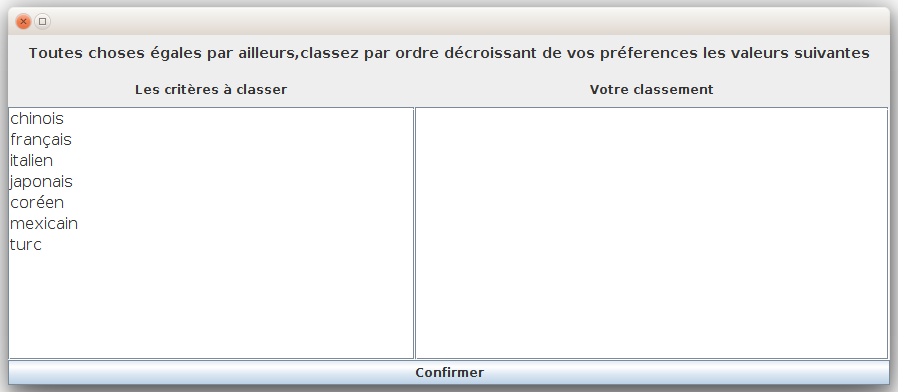
\includegraphics[width=4in]{Figures/pref.png}
		\caption{\label{fig:pref} Interface pour la saisie d'ordre de préférence. Exemple pour le critère de cuisine}
	\end{figure} 
	
	
	\subsection{Hypothèses opérationnelles}
	Nous formulons donc les hypothèses opérationnelles suivantes :
	\begin{itemize}
		\item\textit{\textbf{H1}: Les comportements de complémentarité et de similarité des agents virtuels sont perçus par les participants.}
		
			\subitem $\circ$  Les comportements de dominance attribués par les participants aux agents sont \textit{significativement différents} des comportements de dominance qu'ils se sont auto-attribués.
			\subitem $\circ$ Les comportements de dominance attribués par les participants aux agents sont \textit{similaires} aux comportements de dominance qu'ils se sont auto-attribués.
		
		\item \textit{ \textbf{H2}: Les négociateurs atteignent un gain commun plus important quand les négociateurs établissent une relation de dominance complémentaire.}
			\subitem $\circ$ Le restaurant choisi à la fin de la négociation a une valeur de satisfaction  est significativement plus importante pour les préférences des deux négociateurs dans la condition complémentaire comparé aux autres conditions. 
			
		\item [$\bullet$] \textit{\textbf{H3}: La négociation converge plus rapidement dans le cas où les négociateurs ont une relation de dominance complémentaire.}
			\subitem $\circ$ Les participants engageront plus de tours de négociations pour trouver un compromis dans la condition similaire et neutre comparé à la condition complémentaire.
		
		\item  \textit{\textbf{H4}: Le participant se sent plus à l'aise avec un partenaire qui exprime un comportement complémentaire.}
			\subitem $\circ$ Les scores de \emph{confort} perçus sont plus hauts pour l'agent complémentaire et contrôle que pour l'agent similaire.
			\subitem $\circ$ Les participants trouvent que la négociation est plus aisée avec l'agent complémentaire comparé aux autres agents.
		\item  \textit{\textbf{H5}: La complémentarité dans la relation de dominance augmente l'appréciation entre les négociateurs.}
			\subitem $\circ$ Les participants vont percevoir l'agent complémentaire comme significativement plus appréciable que l'agent similaire ou neutre.
		
	\end{itemize}
	
	\section{Résultats}
	\label{sec:res}
	Nous avons mené une étude intra-sujet dans laquelle 63 participants ont pris part. Cependant deux participants ont été écarté car ils ne remplissaient pas les conditions requises (mauvaises réponses à la majorité des questions de manipulations). Par conséquent, notre étude statistique a été mené sur les 61 participants restants. 
	
	
	%	Nous avons d'abord analyser la perception des comportements de pouvoir lors de la négociation. En effet, avant d'analyser les hypothèses, nous voudrions étudier la perception des comportements de complémentarité et la similarité durant la négociation. 
	\subsection{Perception des comportements des agents}
	

	\begin{table}[t]
		\caption{Différence de perception de dominance entre l'agent et le participant pour chaque comportement} 
		\centering
		
		\begin{tabular}{  >{\centering\arraybackslash}m{1.5cm}  >{\centering\arraybackslash}m{2.2cm}  >{\centering\arraybackslash}m{1.5cm}  >{\centering\arraybackslash}m{1.5cm}  >{\centering\arraybackslash}m{1.5cm}  >{\centering\arraybackslash}m{1.5cm}  >{\centering\arraybackslash}m{1.5cm}}
			\hline\hline
			\textbf{Agent}& Évaluation & \textbf{D1} & \textbf{D2} & \textbf{D3} & \textbf{D4} \\ 
			\hline
			
			\multirow{3}{*} {\textbf{Comp.}}  &  Z-Wilcoxon test  & -4.61 & -5.3 & -6.28 & -0.43 \\ 	
			& p-value & 2.88E-06 & 7.31E-08 & 1.42E-10 & \textbf{0.65 }\\ 
			& Effect size & -0.29 & -0.34 & -0.4 & -0.03\\ 
			\hline
			
			\multirow{3}{*} {\textbf{Similaire}}  &  Z-Wilcoxon test  & -1.57 & -2.21 & -1.45 & -1.33\\ 	
			& p-value & 0.11 & \textbf{0.024} & 0.14 & 0.17 \\ 
			& Effect size & -0.1 & -0.14& -0.09 & -0.08 \\ 
			\hline

			\multirow{3}{*} {\textbf{Neutre}}  &  Z-Wilcoxon test  & -6.23 & -5.72 & -7.056 & -0.77\\ 	
			& p value & 2.52E-10 & 6.85E-09 & 8.19E-13 & \textbf{0.4351} \\ 
			& Effect size & -0.4 & -0.36 & -0.45 & -0.049 \\ 
			\hline \hline
			
		\end{tabular}
		
		\label{tab:domPercption}
	\end{table}
	
	Pour l'analyse des différences entre les comportements de dominance des agents et des participants, des statistiques non-paramétriques ont été utilisées car la normalité des données ne pouvait être assurée. Pour l'analyse principale, le test des rangs signés de Wilcoxon a été appliqué pour évaluer chacun des quatre comportements.
	
	\subsubsection{Perception de complémentarité}
	
	Pour chaque comportement, nous avons comparé la perception des participants de leur comportements de dominance et ceux de l'agent complémentaire avec lesquels ils ont interagi. Les statistiques descriptives sont présentées dans la figure \ref{fig:comp}. 
	
	Les résultats de l'analyse de Wilcoxon ont révélé que les participants ont perçus une différence significative entre leurs comportements et celui de l'agent comme présenté dans la table \ref{tab:domPercption}. Cette différence concerne les comportements \textbf{D1, D2} et \textbf{D3}. Cependant, aucune différence significative n'a été perçu pour le comportement de leader dans la négociation \textbf{D4}. 
	\begin{figure}[h]
		\centering
		% this is wide enough
		\subfloat [Score de perception des comportements de dominance]{
			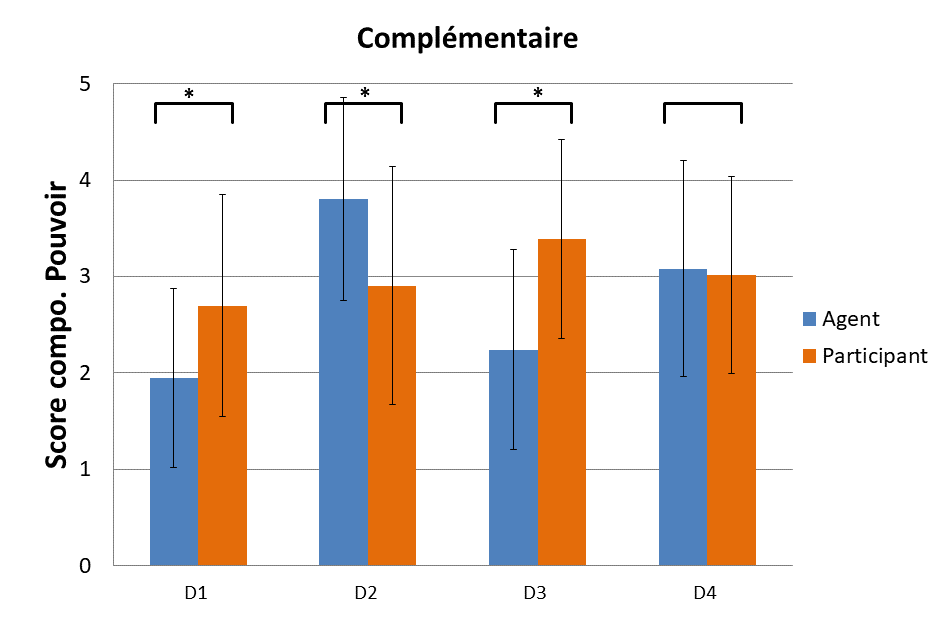
\includegraphics[clip=false]{Figures/chap7/comPow.PNG}
		}
		
		% this has a too narrow subfigure
		\subfloat[Moyenne et écart type dans les comportements de dominance]{
			\begin{tabular}{l c c c c c c}
				\hline\hline
				\textbf{Agent} & Evaluation&  \textbf{D1} & \textbf{D2} & \textbf{D3} & \textbf{D4} \\
				\hline
				
				\multirow{2}{*}{\textbf{Comp.} }& Moyenne & 1,94& 3,80 & 2,24 & 3,08 \\
				& Ecart-type & 0,93 & 1,05 & 1,03 & 1,11 \\
				
				\hline
				\multirow{2}{*}{\textbf{Part.}}& Moyenne & 2,69 & 2,94 & 3,4 & 3,02 \\
				& Ecart-type & 1,14 & 1,23 & 1,03 & 1,02\\
				\hline
				\hline
			\end{tabular}
		}
		\caption{Perception des comportements de dominance avec l'agent complémentaire}
		\label{fig:comp}
	\end{figure}	
	
	\subsubsection{Perception de similarité}
	Nous avons aussi analysé les comportements des négociateurs lors de leurs interactions avec l'agent Arthur. Les statistiques descriptives ont déjà montre une forte similarité dans la perception de tous les comportements (voir la figure \ref{fig:sim}). Nous avons complété l'étude par une comparaison de Wilcoxon a confirmé l'absence de différence significative comme présenté dans la table \ref{tab:domPercption}.  
	\begin{figure}[!tb]
		\centering
		% this is wide enough
		\subfloat[Score de perception des comportements de dominance]{
			\centering
			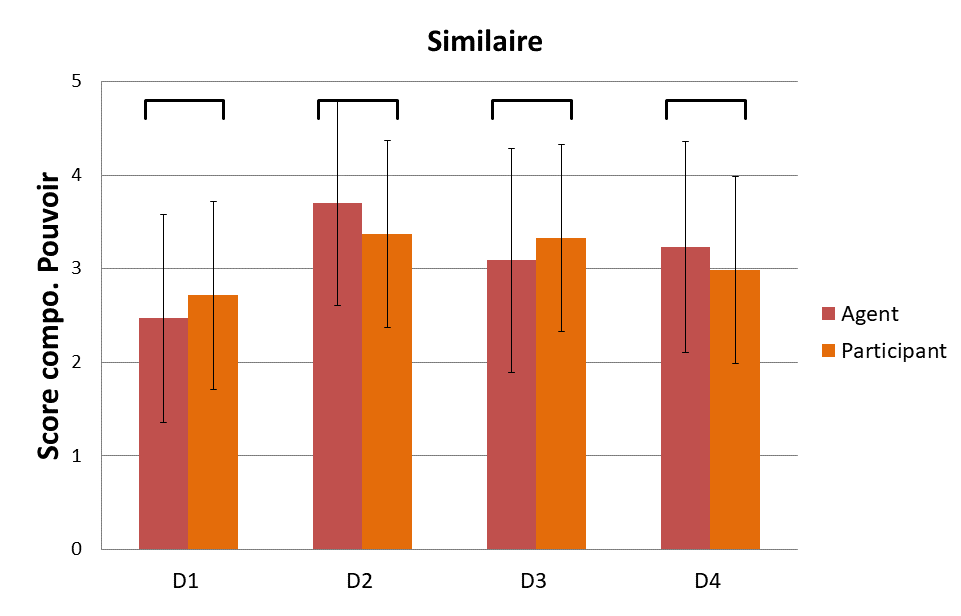
\includegraphics[clip=false]{Figures/chap7/simPow.PNG}
		}
		
		%\vspace{1em}
		% this has a too narrow subfigure
		\subfloat[Moyenne et écart type dans les comportements de dominance]{
			\centering
			\begin{tabular}{l c c c c c c}
				\hline\hline
				\textbf{Agent} & Evaluation& \textbf{D1} & \textbf{D2} & \textbf{D3} & \textbf{D4} \\
				\hline
				
				\multirow{2}{*}{\textbf{Simil.}}& Moyenne & 2,47 & 3,70 & 3,09 & 3,23 \\
				& Ecart-type & 1,11 & 1,10 & 1,19 & 1,12 \\
				
				\hline
				\multirow{2}{*}{\textbf{Part.}}& Moyenne & 2,71 & 3,37 & 3,33 & 2,98 \\
				& Ecart-type & 1,06 & 1,03 & 1,06 & 1,09\\
				\hline \hline
				
			\end{tabular}
		}
		\caption{Perception des comportements de dominance avec l'agent similaire Arthur}
		\label{fig:sim}
	\end{figure}
	
	\subsubsection{Comportement de l'agent neutre}
	
	Nous avons conduit les mêmes études statistiques pour analyser la perception des comportements de l'agent neutre. L'analyse descriptive présentée dans la figure \ref{fig:neutre} montre que les participants ont perçu que l'agent adoptait une stratégie complémentaire pour les comportements \textbf{D1}, \textbf{D2} et \textbf{D3}. Cependant, aucune différence significative n'a été perçu pour le comportement \textbf{D4}.
	
	\begin{figure}[!tb]
		\centering
		% this is wide enough
		\subfloat[Score de perception des comportements de dominance]{
			
			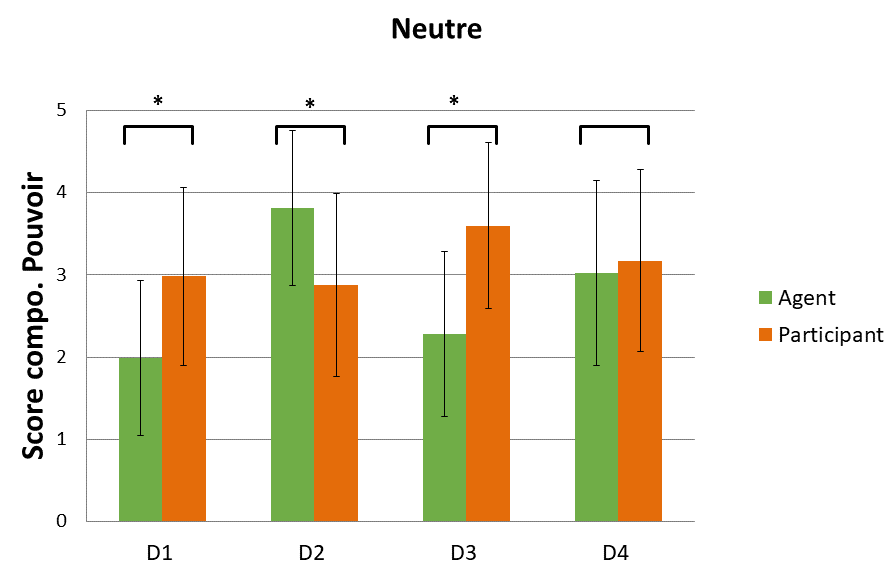
\includegraphics[clip=false]{Figures/chap7/neutrePow.PNG}
		}
		
		%\vspace{1em}
		% this has a too narrow subfigure
		\subfloat[Moyenne et écart type dans les comportements de dominance]{
			
			\begin{tabular}{l c c c c c c}
				\hline\hline
				\textbf{Agent} & Evaluation& \textbf{D1} & \textbf{D2} & \textbf{D3} & \textbf{D4} \\
				\hline
				
				\multirow{2}{*}{\textbf{Neutre}}& Moyenne & 1,99 & 3,81 & 2,28 & 3,02 \\
				& Ecart-type & 0,94 & 0,94 & 1,01 & 1,12 \\
				
				\hline
				\multirow{2}{*}{\textbf{Part}}& Moyenne & 2,98 & 2,88 & 3,60 & 3,17 \\
				
				& Ecart-type & 1,08 & 1,12 & 1,01 & 1,10 \\
				\hline \hline
				
			\end{tabular}
			
		}
		\caption{Perception des comportements de dominance avec l'agent neutre}
		\label{fig:neutre}
	\end{figure}
	
	\subsection{Gain commun}
	Nous avons analysé le gain commun des négociateurs durant les différentes négociations. Nous avons d'abord demandé aux participants leurs ressentis sur la satisfaction du restaurant choisi. Nous avons complété cette analyse par une étude objective dans laquelle nous avons calculé le score de satisfaction du restaurant choisi à partir des préférences du participant et de l'agent. L'ensemble des résultats est présenté en Annexe \ref{chap:Annexe}.
	
		\begin{figure}[h]
		
		\centering
		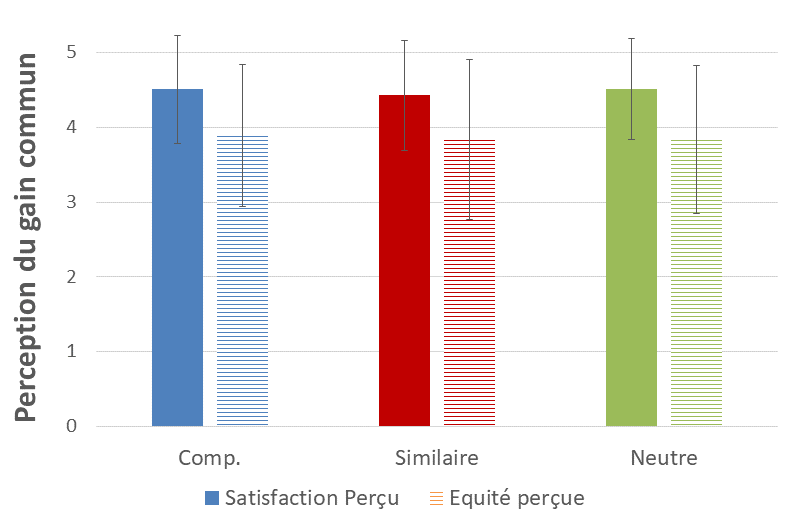
\includegraphics[width= 0.65 \linewidth,clip=false]{Figures/chap7/percpGain.PNG}
		\caption{Perception du gain commun obtenu pour tous les agents \textit{Aucune différence significative entre les agents}}
		\label{fig:gainCom}
	\end{figure}

	\subsubsection{Perception du gain commun} Nous avons demandé aux participants de renseigner leurs degrés de satisfaction du restaurant choisi avec l'agent.
	
	Les résultats sont présentés dans la figure \ref{fig:gainCom}. D'abord, les statistiques descriptives montrent qu'en moyenne les participants étaient satisfaits du restaurant choisi, et ce pour toutes les négociations. Les scores sont plutôt supérieurs à la moyenne pour tous les agents (les valeurs varient entre \emph{3.83} et \emph{4.5} sur une échelle de \emph{5}). 
	
	En outre, nous avons analysé si les participants étaient significativement plus satisfaits du restaurant choisi lors de la négociation avec l'agent Bob qu'avec les autres agents. Nous avons effectué un test de rangs signés de Wilcoxon car la normalité des données n'avait pu être assurée. L'analyse n'a montré aucune différence significative de la perception de gain et d'équité sur le choix du restaurant entre les différents agents. 
	
	\subsubsection{Analyse du gain commun } Concernant l'analyse objective du gain commun atteint à la fin de chaque négociation, nous avons dans un premier temps, récupéré les préférences des participants et des agents avec lesquels avaient interagi. 
	Ensuite, nous avons calculé la satisfiabilité du restaurant choisi pour chaque négociateur en fonction de leurs préférences (\textit{i.e. l'agent et le participant}). Nous avons ensuite, calculé le gain commun atteint à chaque négociation comme \textbf{la moyenne des valeurs de satisfiabilité} des deux négociateurs.  Les résultats obtenus pour chaque agent sont présentés dans la figure \ref{fig:gain}. 
	
		\begin{figure}[h]
		
		\subfloat[Score du gain commun atteint pour tous les agents  \textit{les populations regroupées avec $(*)$ sont significativement différentes }]{
			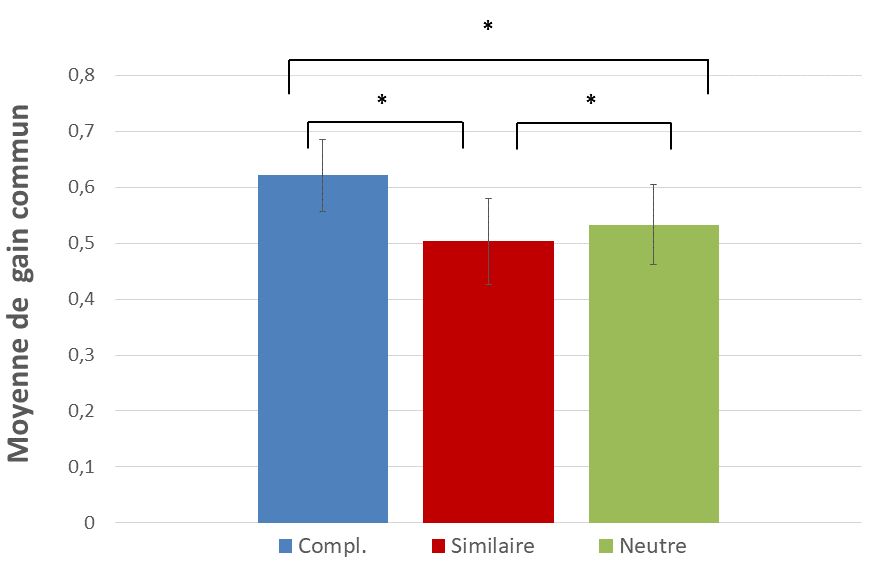
\includegraphics[clip=false]{Figures/chap7/gainCommun.PNG}}
		
		\subfloat [Score du gain commun obtenu par négociation]{
			\centering
			\begin{tabular}{l c c c}
				\hline
				\hline
				\textbf{ }& \textbf{Agent Comp.} & \textbf{Agent similaire} & \textbf{Agent neutre} \\ 
				\hline
				\newline Moyenne & 0.62& 0.5 & 0.53 \\
				\newline Écart type & 0.06 & 0.08 & 0.07 \\
				\hline
				\hline
			\end{tabular}
		}
		\caption{Les résultats obtenus pour le gain commun atteint durant la négociation}
		\label{fig:gain}
	\end{figure}

	Les valeurs de satisfiabilité sont supérieures à la moyenne pour tous les agents. Rappelons que les valeurs de satisfiabilité sont normalisées dans un intervalle $[0, 1]$. Nous avons étudié si les négociateurs avaient atteint un gain commun plus importants en négociant avec l'agent complémentaires comparés aux autres agents. En vue de la distribution normale des valeurs, nous avons appliqué un T-test afin de comparer chaque paire d'agents. Les résultats obtenus sont présentés dans la figure \ref{fig:gain}. L'analyse de la variance a montré une interaction significative entre la relation de dominance et le gain commun atteint lors des négociations. Effectivement, les participants ont atteint un gain commun significativement plus élevé en négociant avec l'agent complémentaire qu'avec l'agent similaire (\emph{t= 8.9, p < 0.01}). La même différence a été perçue en comparant avec l'agent neutre (\emph{t= 6.4, p < 0.01}).
	De plus, les participants ont atteint un meilleur gain commun avec l'agent neutre qu'avec l'agent similaire (\emph{t= 2.3, p = 0.02}).
	

	
	\subsection{Tours de paroles}
	
	Pour l'analyse de l'impact de la relation de dominance sur nombres de tours de paroles, nous avons recueilli le nombre de tours de paroles énoncé durant chaque négociation. Les statistiques descriptives sont présentées dans la figure \ref{fig:tour}. Un test paramétrique a été utilisée car les données suivent une distribution normale. Les résultats montrent que la négociation convergeait significative plus rapidement quand les participants négociaient avec l'agent complémentaire par rapport à l'agent similaire (\emph{t= 2.7, p = 0.003}). De même, la négociation convergeait plus rapidement avec l'agent neutre comparé à l'agent similaire (\emph{t= 4.43, p < 0.01}).  Les résultats sont présentés en Annexe \ref{chap:Annexe}.
	Cependant, aucune différence significative n'a été perçu entre l'agent complémentaire et l'agent neutre (\emph{t= 1.3, p = 0.09}).  
	
	\begin{figure}[!tbh]
		
		\subfloat[Nombre de tours de paroles durant une négociation pour tous les agents \textit{les populations regroupées avec $(*)$ sont significativement différentes}] {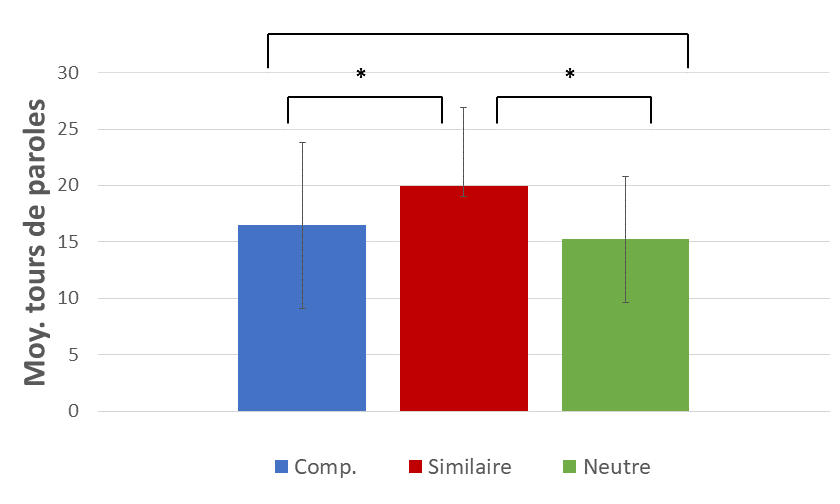
\includegraphics{Figures/chap7/tours.PNG}}
		
		
		\subfloat[Nombre de tours de paroles par négociation]{
			\centering
			\begin{tabular}{ l c c c }
				\hline
				\hline
				\textbf{ }& \textbf{Agent Comp.} & \textbf{Agent similaire} & \textbf{Agent neutre} \\ 
				\hline
				\newline Moyenne & 16.61& 19.94 & 15.13 \\
				\newline Écart type & 7.38 & 6.87 & 5.6 \\
				\hline
				\hline
			\end{tabular}
		}
		\caption{Résultats pour l'hypothèse H3.}
		\label{fig:tour}
	\end{figure}
	
	
	\subsection{Confort}
	
	Les statistiques descriptives sont présentées dans la table \ref{tab:confort}. Les participants se sont globalement sentis à l'aise avec tous les agents.
	Les score de détente ressentie sont au-dessus de 3,4 (sur une échelle à 5 points) pour tous les agents. Au contraire, les scores relatifs à l'anxiété  ressentie sont au-dessous de 2 (sur une échelle à 5 points) pour tous les agents. 
	
	Afin d'analyser une différence dans le confort perçue, nous avons utilisé un test non paramétrique car la normalité n'a pas pu être assurée. Le test de rang signé de Wilcoxon a été appliqué afin d'analyser si les participants se sont sentis plus à l'aise avec l'agent complémentaire qu'avec les autres agents. (Voir résultats en annexe \ref{chap:Annexe}). 
	Les résultats montrent que les participants se sont sentis plus à l'aise avec l'agent complémentaire qu'avec l'agent similaire (\emph{Z= -2.73, p = 0.002})
	avec un effet de taille faible (\emph{e = -0.1}). Cependant, aucune différence significative n'a été perçu entre l'agent complémentaire et l'agent neutre. 
	
	
	\begin{figure}[h]
		
		\subfloat[Score de confort que les participants ont ressenti pour tous les agents. \textit{les populations regroupées avec $(*)$ sont significativement différentes }]{
			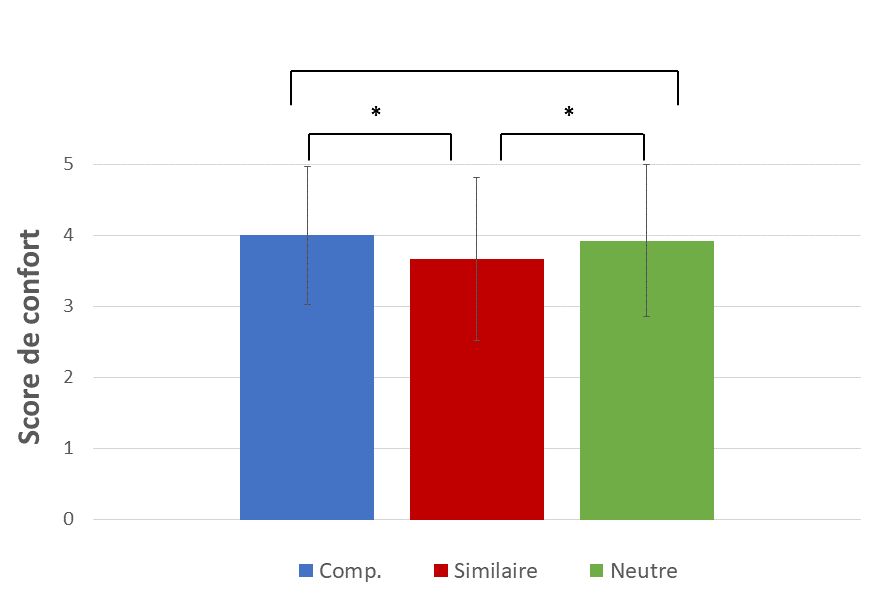
\includegraphics[clip=false]{Figures/chap7/confort.PNG}
		}
		
		\subfloat[L'effet de la relation de dominance sur le confort ressenti pendant la négociation avec l'agent]{
			\centering
			\begin{tabular}{ l l c c c  }
				\hline\hline
				\textbf{ }& & \textbf{Agent Comp.} & \textbf{Agent similaire} & \textbf{Agent neutre} \\ 
				\hline
				\newline \newline\multirow{2}{*} {Détendu} & Moy. &3.79 & 3.47 & 3.79 \\
				\newline  & SD & 1 & 1.2 & 1 \\
				\hline
				
				\newline \newline\multirow{2}{*} {Anxieux} & Moy. & 1.79 & 2.13 & 1.93 \\
				\newline  & SD & 7.38 & 6.87 & 5.6 \\
				\hline\hline
			\end{tabular}
		}
		\caption{Résultats pour la perception du confort durant la négociation.}
		\label{tab:confort}
	\end{figure}	
	\vspace{- 1 em}
	
	\subsection{Appréciation}
	Les statistiques descriptives concernant les scores d’appréciation sont présentées dans la figure \ref{fig:app}. Globalement,
	les scores sont centrés autour de 3.7 (sur une échelle de 5). L'analyse de variance montre l'effet de la relation de dominance sur la perception de l'appréciation. Les résultats sont présentés en annexe \ref{chap:Annexe}.
	
	\begin{figure}[h]
		
		\subfloat[Score d'appréciation perçue pour tous les agents. \textit{les populations regroupées avec $(*)$ sont significativement différentes}]{
			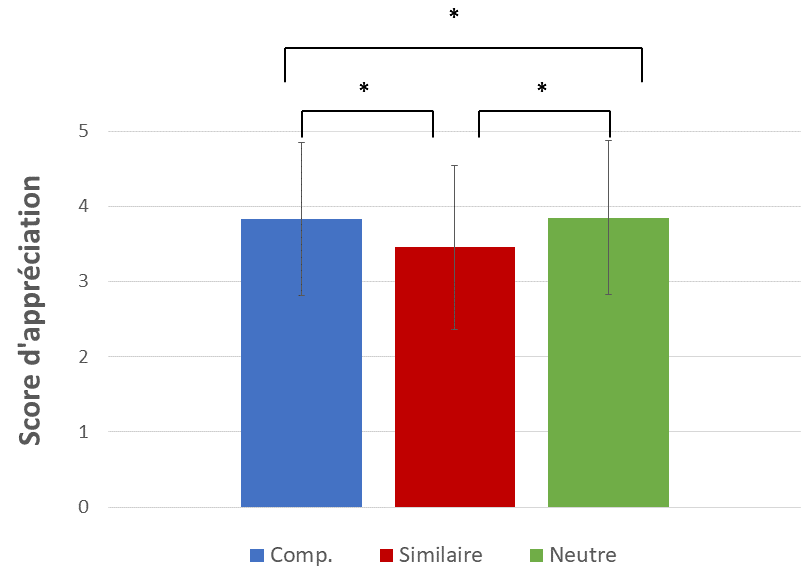
\includegraphics[clip=false]{Figures/chap7/appreciation.PNG}
		}
		
		\subfloat[L'effet de la relation de dominance sur l'appréciation perçue]{			
			
			\begin{tabular}{ l c c c c c }
				\hline\hline
				\textbf{ }& \textbf{Agent Comp.} & &  \textbf{Agent similaire} & & \textbf{Agent neutre} \\ 
				\hline
				\newline Moy. & 3.83 & &3.46 & & 3.85 \\
				\newline SD & 1.01 & & 1.09& &  1.02 \\
				\hline\hline
				
			\end{tabular}
		}
		\caption{Résultats pour la perception de l'appréciation.}
		\label{fig:app}
	\end{figure}
	
	
	Le test de rangs signé de Wilcoxon montre que l'agent complémentaire a été perçu comme significativement plus agréable que l'agent similaire (\emph{p < 0.01, Z = -3.17}). Par ailleurs, l'agent neutre a aussi été perçu comme plus agréable que l'agent similaire (\emph{p < 0.01, Z = -3.3}). Cependant, aucune différence n'a été perçu entre l'agent complémentaire et l'agent neutre (\emph{p = 0.6, Z = -0.31}).
	
	Nous nous sommes aussi intéressés à la facilité de collaboration entre le participant et l'agent. En effet, nous avons demandé aux participants de relater le degré de facilité de négociation avec l'agent. Les résultats sont présentés dans la figure \ref{fig:aise}. En général, les participants ont trouvé que la négociation été aisée avec l'agent complémentaire (\emph{M= 4, SD = 1}) ainsi qu'avec l'agent neutre (\emph{M=3.9, SD =0.99}). Les participants ont perçue la négociation avec l'agent similaire comme moins aisée (\emph{M=3.16, SD = 1.06}). 
	Nous avons ensuite analysé si cette différence de perception été significative. Comme les données ne sont pas normalement distribué, nous avons appliqué le test de rangs signé de Wilcoxon. Les résultats montrent qu'en effet les participants ont trouvé que négocier avec l'agent similaire été significativement moins aisée comparé à l'agent complémentaire (\emph{p < 0.01, Z = -3.86} avec un effet de taille moyen \emph{e = -0.35}) et l'agent neutre (\emph{p < 0.01, Z = -3.61} avec un effet de taille moyen \emph{e = -0.32}).
	Cependant, aucune différence n'a été perçue entre l'agent complémentaire et l'agent neutre.
	\begin{figure}[h]
		
		\subfloat[Évaluation de la collaboration durant la négociation. \textit{les populations regroupées avec $(*)$ sont significativement différentes }]{
			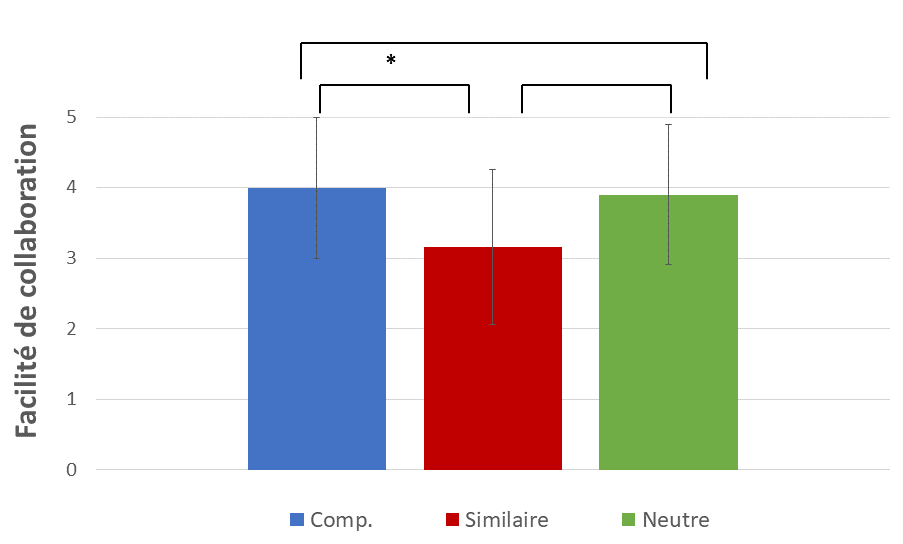
\includegraphics[clip=false]{Figures/chap7/aisee.PNG}
		}
		
		\subfloat[L'effet de la relation de dominance sur la facilité de collaboration]{
			\centering
			\begin{tabular}{ l c c c c c }
				\hline\hline
				\textbf{ }& \textbf{Agent Comp.} & &  \textbf{Agent similaire} & & \textbf{Agent neutre} \\ 
				\hline
				\newline Moy. & 4 & & 3.16 & & 3.9 \\
				\newline SD & 1 & & 1.09  & & 0.99   \\
				\hline\hline
				
			\end{tabular}
		}
		\caption{Résultats pour la facilité de collaboration durant la négociation.}
		\label{fig:aise}
	\end{figure}
	
	
	\section{Analyses complémentaires}
	Dans le chapitre 2, nous présentons la relation de dominance comme une relation interpersonnelle qui s'établie durant l'interaction. 
	Par conséquent, en plus du trais de personnalité, un individu est influencé par l'environnement de l'interaction (\textit{ex.} contexte de l'interaction, rôle social ...). Ces différents paramètres vont créer une certaine relation de dominance qui peut varier d'une interaction à une autre.  
	Afin de vérifier si les participants produisaient différents comportements de dominance durant les différentes négociations, nous avons recueilli la perception de l'agent des comportements de dominance de son interlocuteur.  Les résultats sont présentés dans la figure \ref{fig:dom}.
	
	Nous avons analysé, pour le même participant, la variance des comportements de dominance à travers les trois négociations. Pour ce faire, nous avons utilisé le test de rang signé de Wilcoxon car la normalité des données n'a pu être assurée. 
	
	Les résultats montrent les comportements de dominance des participants variaient d'une interaction à une autre. En effet, le test de Wilcoxon révèle une différence significative entre les comportements perçus par l'agent complémentaire et l'agent similaire (\emph{p<0.01, Z = -3.35}). Ces mêmes résultats sont observés en comparant la perception de l'agent complémentaire et l'agent neutre (\emph{p< 0.01, Z = -3.88}).
	Toutefois, aucune différence entre l'agent similaire et l'agent neutre n'a été vérifié (\emph{p = 0.6, Z = 0.44}). 
	
	Ces résultats suggèrent que les participants ont adopté une stratégie de négociation différente en fonction de la relation établie avec l'agent. 
	
	\begin{figure}[h]
		
		\subfloat[Évaluation de comportements de dominance des participants perçus par les agents. \textit{les populations regroupées avec $(*)$ sont significativement différentes }]{
			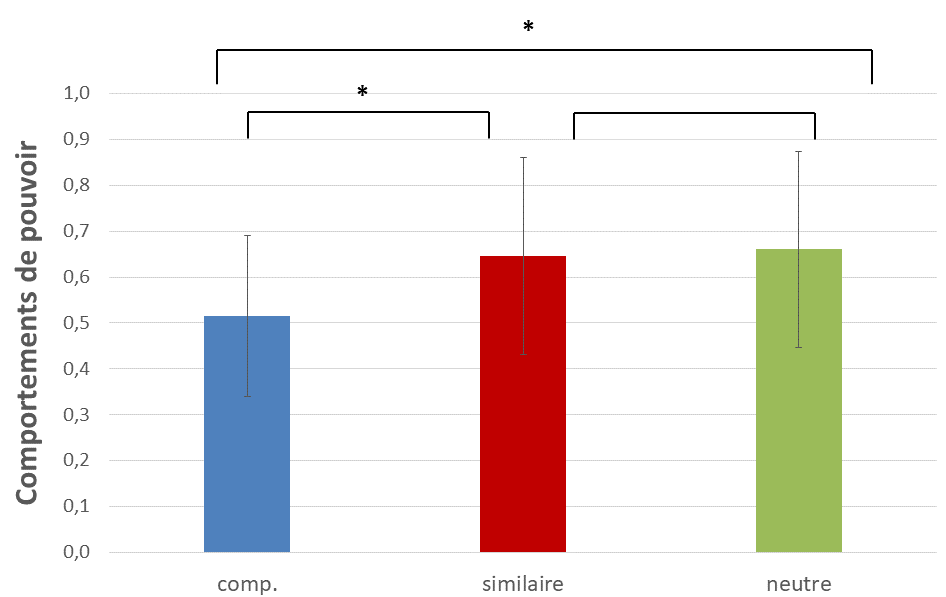
\includegraphics[clip=false]{Figures/chap7/pow.png}
		}
		
		\subfloat[Perception de l'agent des comportements de dominance exprimés par les participants]{
			\begin{tabular}{ l c c c c c }
				\hline
				\hline
				\textbf{ }& \textbf{Agent Comp.} & &  \textbf{Agent similaire} & & \textbf{Agent neutre} \\ 
				\hline
				\newline Moy. & 0.51 && 0.64 && 0.66 \\
				\newline SD & 0.17 && 0.21 && 0.219   \\
				\hline
				\hline
			\end{tabular}
		}
		\caption{Résultats pour la variation des comportements de dominance à travers les interactions.}
		\label{fig:dom}
	\end{figure}
	
	\section{Discussion}
	\label{sec:discussion}
	En général, toutes nos hypothèses ont été validées. Ces résultats appuient la validité de notre modèle négociation collaborative et de théorie de l'esprit dans le cadre d'une interaction agent/humain.   
	
	\subsection{Perception des comportements des agents}
	Notre hypothèse H1 (\textit{les comportements de complémentarité et de similarité des agents virtuels sont perçus par les participants}) est partiellement validée. 
	
	Quatre comportements de dominance ont été pris en compte pour mesurer la stratégie de négociation. 
	Les participants ont été en mesure de distinguer une différence significative de trois comportements sur quatre entre leurs stratégies et celle de l'agent complémentaire.
	
	En effet, les participants ont perçu une différence entre leurs niveaux d'exigences et de concessions \textbf{D3}, \textbf{D2}, ainsi que la prise en compte des préférences de l'autre \textbf{D1}. Cependant, aucune différence n'a été perçu concernant les comportements de leadership durant la négociation \textbf{D4}. 
	
	Concernant, les comportements de l'agent neutre, ce dernier a été perçu comme significativement complémentaires aux utilisateurs pour les comportements \textbf{D1}, \textbf{D2} et \textbf{D3}. 
	Toutefois, comme l'agent complémentaire, aucune différence n'a été perçue dans les comportements relatifs à \textbf{D4} entre l'agent neutre et les participants. 
	
	Nous avons étudié les données afin de comprendre pourquoi les participants ne percevaient pas de différence dans les comportements de leadership. 
	
	Concernant l'agent complémentaire, les comportements de leaderships ont pu être masqué à cause de  sa stratégie d'adaptation qui modifié ses comportements de dominance à chaque tour de parole.
	
	En outre, l'aspect collaboratif de la négociation pourrait avoir atténué la perception du leadership dans la négociation ce qui pourrait expliquer le cas de l'agent neutre. 
	
	Enfin, l'absence de résultats pour les deux agents nous amènent à nous questionner sur les items proposés pour mesurer le leadership. 
	Il serait intéressant de faire une évaluation post-hoc afin de demander aux participants le types de comportements qu'identifieraient le leadership durant la négociation.
	
	En parallèle, les participants ont perçu une similarité entre leurs comportements et ceux de l'agent similaire. En moyenne, pour chaque comportement, les valeurs assignés en auto-attribution et en hétéro sont très proches. De plus, l'absence de différence significative appuie ce résultat. Nous sommes conscients que l'absence de différence n'est pas une assurance de similarité de perception. Cependant, il est difficile de trouver un calcul statistique qui assure la similarité entre deux populations.
	
	D’un point de vue plus général, les résultats obtenus appuient la cohérence de notre modèle de décision tant sur la perception des comportements de dominance que sur la capacité de l'agent à percevoir les comportements de son interlocuteur et de s'y adapter correctement.  
	
	Par ailleurs, la perception des comportements de l'agent neutre comme complémentaires à ceux des participants soutient que la relation interpersonnelle de dominance qui s'établie au cours de l'interaction est complémentaire \cite{burgoonnonverbal}. En effet, indépendamment des deux autres agents où nous avions manipulé l'adaptation de l'agent, dans la condition neutre l'agent ne s'adapte pas aux comportements du participant. Néanmoins, les résultats démontrent que le participant s'est adapté aux comportements exhibés par l'agent et a ainsi établie une relation interpersonnelle de dominance complémentaire.
	
	\subsection{Gain commun}
	Notre seconde hypothèse (\textit{Les négociateurs atteignent un gain commun plus important quand les négociateurs établissent une relation de dominance complémentaire.}) est validée. 
	
	Nous avons en premier temps demandé aux participants de relater leur avis sur le restaurant choisi pour chaque négociation.
	En général, les participants ont été satisfaits du choix final et le trouvaient équitable pour toutes les négociations. 
	En analysant la valeur de satisfiabilité du restaurant choisi pour les préférences des participants (voir table \ref{tab:gainPerceptif}), les valeurs étaient autour de 0.7 (\emph{min =0.69, max = 0.73}). 
	
	Cependant, en analysant la valeur de satisfiabilité pour les préférences de l'agent,  en moyenne, seul l'agent complémentaire a pu converger vers un restaurant qui respecte ses préférences (\emph{M = 0.53, SD = 0.2}). 
	
	
	\begin{table}
		\centering
		\caption{Moyenne des valeurs de satisfiabilité du restaurant choisi pour chaque négociateur} 
		\begin{tabular} {lcccccccc}
			\hline
			\hline
			& \multicolumn{2}{c}{Agent Comp.} & & \multicolumn{2}{c}{Agent similaire}& & \multicolumn{2}{c}{Agent neutre} \\ % column 4 blank, for spacing
			\cline{2-3} \cline{5-6} \cline{8-9} % horizontal lines connecting cols. 2-3, 5-6
			& Part. & Agent & & Part. & Agent & &  Part. &Agent \\ \hline
			Moy. &0,71 & 0,53 & &  0,69 & 0,33 & & 0,73 & 0,34 \\
			SD & 0,2 & 0,24 & &  0,18 & 0,19 & & 0,18 & 0,16 \\
			\hline
			\hline
		\end{tabular}
		\label{tab:gainPerceptif}
		
	\end{table}
	
	Concernant l'agent similaire, la moyenne de satisfiabilité est assez basse. Ceci est causé par le fait que les négociateurs ne communiquaient pas bien durant la négociation. Par conséquent, la négociation durait plus longtemps causant la chute de la courbe de concession $Self$. De ce fait, l'agent faisait plus de concession et finissait par accepter un restaurant dont la satisfiabilité n'était pas élevée (\emph{M = 0.33, SD = 0.18}).
	
	Concernant l'agent neutre qui n'est pas très dominant, il est normal que dans la majorité des cas, la courbe de concession finissait par décroitre menant l'agent à faire des concessions importantes. Ceci explique la moyenne de satisfiabilité atteinte par l'agent neutre  (\emph{M = 0.34, SD = 0.16}).
	
	Cette analyse confirme les résultats de l'étude objective menée.
	Pour toutes les négociations, nous avons comparé le gain commun et nous avons observé qu'il était significativement plus important durant les négociations avec l'agent complémentaire comparé aux autres agents. De plus, les négociateurs avaient de meilleurs gains durant la négociation avec l'agent neutre comparé à l'agent similaire. Ceci prouve que la relation complémentaire qui s'est installé durant la négociation avec l'agent neutre a permis un meilleur échange d'information. 
	
	Ces résultats confirme que les négociateurs communiquent mieux et par conséquent négocient mieux dans le cadre d'une relation complémentaire de dominance.  
	
	
	\subsection{Tours de paroles}
	Notre hypothèse H3 (\textit{La négociation converge plus rapidement dans le cas où les négociateurs ont une relation de dominance complémentaire}) est validée. En effet, la négociation convergeait en moyenne plus rapidement quand une relation de dominance complémentaire s'établissait entre l'agent et le participant. De plus, dans cette même condition le gain commun atteint par les négociateurs était plus important. Ainsi, ces résultats appuient les théories de  psychologie sociales selon lesquelles la relation interpersonnelle de dominance améliore la coordination et l'échange d'informations.
	
		
	En ce qui concerne l'agent neutre, la négociation convergeait rapidement à cause de deux raisons. Premièrement, avec une valeur de dominance initialisée à 0.5, l'agent avait un niveau d'exigence moyen ce qui facilitait le processus pour trouver un compromis. 
	Deuxièmement, d'après nos résultats, dans cette condition, une relation complémentaire de dominance s'était établie entre les négociateurs ce qui facilitait la coordination. 
	
	En conclusion, la relation interpersonnelle de dominance améliore la coordination et l'échange d'information qui résulte en des processus de négociation court et plus efficaces. 
	
	\subsection{Appréciation de l'agent}
	Nos hypothèses H4 (\textit{Le négociateur se sent plus à l'aise avec un partenaire qui exprime un comportement complémentaire})  et H5  (\textit{La complémentarité dans la relation de dominance augmente l'appréciation entre les négociateurs.}) sont validées. 
	
	Pour l’appréciation, les scores sont au-dessus de la moyenne pour tous les agents. Ce pourrait être le reflet d’un léger biais positif envers les agents. Toutefois, l'analyse des différences a révélé que les participants ont significativement plus apprécié la négociation avec l'agent complémentaire que l'agent similaire. De même, les participants ont jugé que l'agent neutre était aussi plus agréable que l'agent similaire. 
	
	En outre, nous avons analysé le confort ressenti lors de la négociation. Globalement, les participants se sont sentis détendus durant la négociation et ont trouvé la négociation confortable avec tous les agents.  
	
	L'analyse de variance a révélé que les participants se sont plus sentis à l'aise avec l'agent complémentaire qu'avec l'agent similaire. Cependant, aucune différence n'a été perçu entre l'agent complémentaire et l'agent neutre, et entre l'agent neutre et l'agent similaire.
	
	En plus du confort, nous avons analysé la facilité de collaborer avec l'agent durant la négociation. Les résultats montent que les participants ont perçu le processus de négociation comme plus aisé avec l'agent complémentaire et l'agent neutre qu'avec l'agent adoptant une stratégie similaire à la leurs. 
	
	Ces résultats confirment nos hypothèses. Les participants préfèrent négocier avec un partenaire avec lequel ils ont établi une relation complémentaire qu'avec un négociateur qui exhibe des comportements de dominance similaires. 
	
	
	\section{Conclusion}
	Pour cette quatrième étude, nous avions pour objectif d'étudier l'effet de la relation de dominance sur la négociation entre un agent et un participant humain. Nous nous sommes basés sur les travaux de Tienders et Wiltermuth \cite{wiltermuth2009benefits,tiedens2003power} qui affirment que la complémentarité dans la relation de dominance avait un impact positif sur la négociation. 
	
	Nous avons implémenté trois agents négociateurs adoptant trois stratégies différentes, un agent complémentaire, un agent similaire et un agent neutre. 
	63 participants ont pris part à  des négociations collaboratives avec ces agents dans le but de trouver un restaurant qui satisfassent leurs préférences. 
	
	Les résultats ont confirmé la majorité de nos hypothèses et nous ont permis d'aller plus loin dans l'analyse des comportements de dominance dans la négociation. 
	
	D'abord, nous avons pu valider notre modèle de la théorie de l'esprit dans le cadre d'une interaction avec un utilisateur humain. 
	Les résultats montrent que les participants ont été capables de percevoir une différence dans les stratégies qu'adoptaient les agents. Ceci nous permet de valider la robustesse des prédictions de notre modèle. 
	
	Par ailleurs, toutes les hypothèses relatives à l'effet positif de la relation de dominance complémentaire ont été validées. Quand les négociateurs établissaient une relation de dominance complémentaire, ils atteignaient un meilleur gain commun et ceux dans un délai plus court comparés aux autres configurations. La négociation était vécue comme plus agréable et confortable et les négociateurs semblaient mieux collaborer. 
	
	Les résultats ont aussi révélé des comportements qui soutiennent les travaux en psychologie sociale. En effet, en analysant les comportements exprimés lors des négociations avec l'agent neutre, nous nous sommes rendu compte qu'une relation complémentaire de dominance s'était installé entre les négociateurs. Ces résultats appuient la définition de Dunbar and Burgoon \cite{dunbar2005perceptions} qui affirment que la relation de dominance est forcément complémentaire. En outre, la relation de dominance étant interpersonnelle, elle s'établie durant l'interaction. Ce point a aussi été validé par nos analyses qui nous ont permis de montrer que les participants ont adopté des comportements de dominance différents d'une négociation à une autre. Cela suggère que les négociateurs s'adaptent à leur interlocuteur pour définir une relation de dominance propre à l'interaction. 

\part{Conclusion}

\chapter{Conclusion}

\begingroup
\parindent=0em
\etocsettocstyle{\rule{\linewidth}{\tocrulewidth}\vskip0.5\baselineskip}{\rule{\linewidth}{\tocrulewidth}}
\emph{\textbf{Sommaire}}
\localtableofcontents 
\clearpage
\endgroup


Cette thèse s'est intéressée à la simulation d'une relation interpersonnelle de dominance entre un agent conversationnel et un humain.
Nous nous plaçons dans le contexte des environnements collaboratifs dans lesquels l'agent partage des objectifs communs avec l'utilisateur. Dans le cadre de ce type d'interaction, les négociations sont fréquentes afin de mettre en œuvre des stratégies qui vont résoudre les conflits liés à ces tâches communes. 
L'étude de l'existant a montré qu'une relation sociale s'établissait entre les interlocuteurs. Cette dernière influençait leurs stratégies d'interaction et plus particulièrement les stratégies de négociation. La relation de dominance est parmi les relations les plus étudiées dans le contexte de négociation humain/humain. 

Nous avons choisi de nous intéresser à la modélisation de cette relation interpersonnelle entre un agent et un humain et d'étudier son impact sur le processus de négociation.  Nous rappelons dans ce chapitre nos contributions majeures, les résultats obtenus et nous terminons par les perspectives sur le court et long terme. 

\section{Contributions}

La première partie de ce travail était consacrée à construire un état de l'art regroupant les travaux en psychologie sociale et en informatique.  Sur l'aspect psychologie, nous nous sommes penchés sur les recherches étudiant la dominance dans les interactions. Nous avons présenté les différents travaux autour de ce concept, comme trait de personnalité, statut ou relation interpersonnelle.

Nous avons détaillé sa manifestation dans les interactions tant sur le niveau verbal et non verbal. Ensuite, nous avons expliqué la manifestation des comportements de dominance sur un niveau stratégique au cours de négociations humain/humain.

Cet état de l'art nous a permis d'identifier les comportements récurrents dans les négociations qui sont liés à la relation de dominance.

Concernant les travaux en informatique, nous avons présenté les contributions majeures dans la modélisation de systèmes de négociation autonomes. Nous avons discuté l'évolution de ce domaine vers l'intégration de comportements sociaux afin d'enrichir les stratégies de négociation autonome. 

Ces travaux nous ont guidé dans la proposition de notre principale contribution de cette thèse, à savoir, un modèle de négociation collaboratif dont les stratégies de négociation sont régies par des comportements de dominance.

Le système de négociation collaborative proposé est composé de trois composantes principales.

D'abord, nous avons proposé un domaine de négociation générique, inspiré des travaux en négociation multicritères. Il permet à l'agent de négocier sur des thèmes variés. De plus, il dispose d'un modèle de préférences d'ordre partiel. L'agent dispose donc de préférences qui guident sa prise de décision rationnelle durant la négociation.

En parallèle, le modèle de communication à base d'actes de dialogue permet à l'agent d'échanger des informations et de négocier avec son interlocuteur. Ces actes de dialogues sont accompagnés d'une formalisation en langage naturel afin de rendre l'interaction plus naturelle et flexible à l'évolution de la négociation.

\subsection{Décision basée sur les comportements de dominance}

La partie essentielle de ce modèle de négociation est le modèle décisionnel de l'agent. Nous avons identifié trois principes de comportements liés à la dominance dans les travaux  en psychologie sociale. Chacun de ces principes a été implémenté dans le processus décisionnel de l'agent.

En effet, à partir de sa position sur le spectre de dominance, l'agent va exprimer ses stratégies de concessions et d'exigences spécifiques. Il va donner plus de poids à ses préférences et essayer de contrôler la négociation. 

Une expérimentation a ensuite été mise en place afin de vérifier la perception des comportements de dominance exprimés par nos agents.

Nous avons conduit une première étude agent/agent où des dyades dans lesquels des agents avec des comportements dominants ont négocié avec des agents soumis. Les participants ont joué le rôle de juges externes afin d'évaluer les comportements des agents dans les dialogues de négociation produits. 

Les résultats obtenus confirment que les participants étaient capables de distinguer différents comportements de dominance d'un agent à un autre. Nous avons complété cette expérimentation par une étude agent/humain. 

Dans cette étude, les participants ont négocié avec deux agents, un agent dominant et un agent soumis. Le but était d'évaluer si les participants percevaient une différence significative entre les deux agents et identifiaient leurs comportements de dominance.

Les résultats suggèrent que les participants percevaient les comportements de dominance exprimés par les agents. En effet, l'agent dominant était perçu comme plus égocentrique et plus exigent et tentait contrôler la négociation alors que l'agent soumis manquait d'initiatives et prenait en compte les préférences de son interlocuteur. Cependant, peu de différences ont été perçues sur les comportements liés aux concessions dues à une limite de notre méthodologie. En effet, nous n'avons pas pris en compte l'impact de la distance des préférences pour la mise en place de l'étude. En conséquence, sur beaucoup de dyades les participants avaient des préférences similaires avec l'agent dominant et des préférences opposées avec l'agent soumis. 

Globalement, les résultats de cette expérimentation suggèrent que les comportements de dominance implémentés sont correctement perçus par les participants. Ces résultats nous ont encouragés dans la suite de nos travaux. 

En effet, afin de simuler une relation interpersonnelle de dominance, l'agent doit reconnaitre les comportements de dominance de son interlocuteur afin d'adopter un comportement complémentaire. Cette adaptation crée une relation interpersonnelle de dominance.  

\subsection{Simulation des comportements de l'interlocuteur}

Notre seconde contribution est l'extension de notre modèle de négociation collaborative pour qu'il raisonne sur les comportements de dominance d'un interlocuteur. Ce modèle est crucial, car à travers ces prédictions, l'agent révise ses comportements de dominance dans le but de simuler une relation interpersonnelle de dominance avec son interlocuteur. 

Pour la mise en œuvre ce modèle, nous nous sommes inspirés des travaux en théorie de l'esprit, et plus particulièrement, l'approche \emph{simulation-theory}. Par conséquent, nous avons utilisé le modèle décisionnel de l'agent pour qu'il puisse prédire les comportements de dominance de son interlocuteur. 

Pour ce faire, nous avons dû adapter le modèle décisionnel de l'agent pour qu'il puisse prédire les comportements de dominance à chaque tour de parole, avec seulement une connaissance partielle des préférences de l'interlocuteur. 

Nous avons validé la pertinence des prédictions dans une étude agent/agent. Nous avons généré plusieurs dyades d'agents négociateurs (au total $1080$ dyades). En plus de négocier avec l'autre, chaque agent devait deviner la valeur de dominance de son interlocuteur.

Les résultats obtenus montrent que les prédictions étaient correctes dans $96\%$ des cas avec un temps de raisonnement court. 

\subsection{Impact de la complémentarité de la dominance sur la négociation}

Notre modèle de négociation collaborative enfin implémenté, nous avons étudié l'impact de la relation interpersonnelle sur le processus de négociation. 

Les travaux en psychologie sociale stipulent qu’une relation interpersonnelle de dominance complémentaire améliore l’échange d’information et mène à un meilleur gain commun des négociateurs.

L’expérience de la négociation est mieux vécue et une relation d’appréciation s’établit entre les négociateurs. 

Nous avons manipulé trois conditions pour la création des dyades de négociation. Dans la première dyade, l'agent adoptait un comportement complémentaire à celui du participant. En revanche, dans la seconde dyade, l'agent a été manipulé pour exprimer des comportements de dominance similaire à ceux détectés chez le participant. Enfin, dans la dernière dyade l'agent adopte un comportement neutre et ne s'adapte pas à son interlocuteur.

Les résultats ont confirmé la majorité de nos hypothèses, ou les dyades complémentaires atteignaient de meilleurs gains communs. Par ailleurs,  la négociation était vécue comme plus agréable et confortable. Enfin, les négociateurs semblaient mieux collaborer. 

Néanmoins, il est nécessaire de garder à l’esprit que l’expérimentation informatique n’est pas une validation en soi d’un modèle psychologique. En effet, les études que nous avons menées évaluent la perception des comportements générés par notre implémentation. Ce processus étant subjectif, d'autres modèles informatiques mêmes sans aucune base théorique peuvent atteindre les mêmes résultats que ceux obtenus par notre modèle.

L'intérêt de faire une étude expérimentale réside dans la réflexion bidirectionnelle qu’elle nourrit par rapport au concept implémenté que par rapport aux choix computationnels faits \cite{faur2016approche}.

\section{Perspectives à court et à long terme}

À l’issue des travaux de cette thèse, nous avons relevé quelques perspectives à explorer dans des travaux futurs.

\subsection{Traits individuels des négociateurs}

La première perspective a pour but de pallier à la limite principale de cette thèse. Le modèle de négociation n'a été testé que pour une seule interaction avec un contexte applicatif basique. Cependant, les environnements collaboratifs impliquent généralement des interactions à répétitions avec un contexte applicatif précis. Par conséquent, les traits individuels des interlocuteurs sont à prendre en compte pour la simulation de la relation interpersonnelle. 

Le contexte applicatif a pour conséquence de définir les rôles des interlocuteurs dans l'interaction qui définira leur statut hiérarchique. Notre modélisation initie la relation de dominance sans prérequis, et le comportement de l'agent est donc neutre. Cependant, en fonction du rôle joué par l'agent, son comportement de dominance doit être initié en conséquence. Par exemple, un agent jouant un rôle de tuteur va être initialisé dans le haut spectre de dominance. 

Par ailleurs, les interactions répétées, vont faire resurgir les traits individuels de chaque interlocuteur et vont affecter l'évolution de la relation interpersonnelle et les comportements exhibés. Il devient essentiel à ce point de les considérer pour rendre l'interaction plus crédible.

\subsection{Expressivité de l'agent}

Un premier axe à étudier sur le long terme est l'enrichissement des stratégies de communication de l'agent. Ce dernier ne communique qu'à travers des actes de dialogue dont le texte en langage naturel est codé manuellement. Cependant, nous avons montré dans la section \ref{sec:manifesationDom} que les comportements de dominance s'expriment aussi avec des comportements verbaux et non verbaux.

Il est donc nécessaire d'améliorer l'expressivité de l'agent afin de rendre ses stratégies de négociation saillantes dans la négociation. 

\subsubsection{Comportement verbal}

La première étape vise à améliorer le style linguistique de l'agent. Nous avons montré dans la section \ref{sec:communication} que la formalisation des actes de dialogue en langage naturel était neutre. 

Nous cherchons donc à donner pour chaque acte de dialogue une formalisation spécifique en fonction de la dominance de l'agent. Les travaux en psychologie sociale ont montré que les individus dominants exprimaient clairement leurs préférences. En revanche, les personnes soumises exprimaient des hésitations et ne rendaient pas leurs préférences explicites.  Ceci est soutenu par la collecte de données que nous avons effectuée.

Par exemple, dans le second dialogue enregistré (voir figure \ref{fig:DSP}), les individus utilisaient deux styles linguistiques différents pour le même acte de dialogue \emph{StatePreference}. Par exemple, dans le \emph{DS1} l'interlocuteur B exprime qu'il n'aime pas vraiment les crêperies sur Paris en insinuant uniquement qu'il a vécu trois ans à Rennes et ce n'est qu'en \emph{DS2} qu'il explique trouver les crêperies sur Paris moyenne.

À l'opposé, l'interlocuteur A qui avait un comportement dominant, affichait ses préférences comme montrées dans le \emph{DS3}:

\begin{minipage}{\textwidth}     {\ttfamily
		
		\begin{addmargin}[1em]{2em}% 1em left, 2em right
			
			\vspace{0.5em}
			
			\hspace*{3mm} \textbf{B:}  Sinon j'aime bien japonais 
			
			\textbf{A:} \textbf{Je n'aime pas du tout} le japonais.
			
			\hspace*{3mm}     \textbf{B:} tu n'aimes pas tout ce qui est poisson cru ... 
			
			\textbf{A:}  \textbf{je n'aime pas trop la cuisine asiatique encore moins japonais}.
			
			\hspace*{3mm}     \textbf{B:} \textbf{Je n'aime pas trop }les sushis déjà.
			
			\textbf{A:} \textbf{Non je ne suis pas trop} cuisine asiatique        \vspace{1.5em}      \end{addmargin}     } 
	
\end{minipage}

\subsubsection{Comportement décisionnel}

La seconde possibilité est d'améliorer l'expressivité sur un niveau décisionnel. En effet, l'argumentation est un processus important durant la négociation, qui permet aux négociateurs de persuader et de convaincre leurs interlocuteurs. L'argumentation dans la négociation a déjà fait l'objet de plusieurs travaux en négociation automatique \cite{toni2010argumentative,oliva2010argumentation}. Cependant, ces travaux se focalisent toujours sur une négociation rationnelle. Il serait intéressant d'étudier comment les comportements de dominance vont affecter les stratégies d'argumentations et leurs expressions dans la négociation.

\subsubsection{Comportement non verbal}

La dernière perspective serait d'intégrer le modèle de négociation collaborative dans un agent incarné. Le but est de doter l'agent de comportements non verbaux. Nous avons présenté dans le chapitre \ref{chap:etat}, plusieurs contributions en informatique affective qui ont implémenté des comportements non verbaux de dominance dans des agents incarnés. Ces comportements ont eu un impact direct sur l'interaction et sur les stratégies de négociation \cite{de2011effect,de2015humans}. 

Sur la base que l'agent soit doté de comportements non verbaux, il est intéressant de continuer d'étudier l'impact des affects et des émotions sur les stratégies de négociation.  En effet, des chercheurs en psychologie sociale \cite{van2006power} ont montré que l'expression de  joie et de colère combinée aux comportements de dominance avait un impact direct sur la négociation. Les négociateurs concédaient plus à un négociateur dominant qui exprimait de la colère qu'à un négociateur joyeux. 

Ces perspectives vont dans la continuité des recherches qui visent à améliorer la crédibilité des interactions d'un agent virtuel et un utilisateur humain. Ceci est d'autant plus important dans les environnements collaboratifs où les interactions ont un rôle important dans l'échange d'information et l'amélioration de la collaboration et la bonne entente.  


%\addtocontents{toc}{\protect\clearpage} % <--- just debug stuff, ignore

%\include{multiToC} % <--- just debug stuff, ignore for your documents
% ********************************************************************
% Backmatter
%*******************************************************
\appendix
%\renewcommand{\thechapter}{\alph{chapter}}
\cleardoublepage
\part{Annexes}
\begin{appendix}


\section{Gain commun atteint dans la négociation}

	\subsection{Perception du gain commun}

\begin{table} [h]
	
	\begin{tabular}{ l c c c c }
		\hline\hline
		\textbf{ }& & \textbf{Comp. >Similaire} & \textbf{Comp. >Neutre} & \textbf{Neutre >Similaire} \\ 
		\hline
		
		
		\multirow{3}{*} {Équité}  &  T-test  & \\ 	
		& p-value & \\ 
		\hline
		
		\multirow{3}{*} {Satisfaction}  &   T-test  &  &  &   \\ 	
		& p-value &  &   &   \\ 
		\hline
	\end{tabular}
	\caption{Analyse du gain commun atteint par tous les agents}
\end{table}

\subsection{Satisfaction du choix final}

	\begin{table}[h]
		
		\begin{tabular}{ c c c c }
			\hline\hline
			 & \textbf{Comp. >Similaire} & \textbf{Comp. >Neutre} & \textbf{Neutre >Similaire} \\ 
			\hline \hline
			
				  T-test  & 8,9 & 6,4 &  2,3 \\ 	
				p-value & 1,74E-12 &  2,884E-08 & 0,025  \\ 
			\hline
			\hline
			
			
			
		\end{tabular}
		\caption{Analyse du gain commun atteint par tous les agents}
	\end{table}
\vspace{-1 em}

\section{Tours de paroles par négociation}

\begin{table}[t]
	
	\begin{tabular}{ c c c c }
		\hline\hline
		& \textbf{Comp. < Similaire} & \textbf{Comp. < Neutre} & \textbf{Neutre < Similaire} \\ 
		\hline\hline
		
		T-test  & 3.33 & 1.49 &  5.56 \\ 	
		p-value & 0.0007 &  0,06 & 2.595e-07 \\ 
		\hline
		\hline
	
		
		
	\end{tabular}
	\caption{Analyse du gain commun atteint par tous les agents}
\end{table}


\section{Appréciation et confort durant la négociation}

\begin{table}[h]
			\centering
	\begin{tabular}{ l c p{3 cm} p{3 cm} p{3 cm} }

		\hline\hline
		\textbf{ }& & \textbf{Comp.>Sim.} & \textbf{Comp.>Neutre} & \textbf{Neutre>Sim.} \\ 
		\hline
		
		\multirow{3}{*} {Appréciation}  & Z-Wilcoxon& -3,17 & -0,32 & -3,29	\\ 	
										& p-value &	0,0005 & 0,6298 & 0,0003  \\ 
										& Effect size & -0,20 & -0,02 & -0,21 \\ 
		\hline
		
		\multirow{3}{*} {Confort}  &Z-Wilcoxon& -2,74 & -0,81 & -2,62 \\
									& p-value & 0,0026 & 0,2 & 1 \\ 
									& Effect size & -0,18 & -0,05 & -0,17 \\ 
		
		
		\hline\multirow{3}{*} {Collaboration}  &  Z-Wilcoxon  & -3,86 & -0,91 & -3,61\\ 	
		& p-value & 4,28E-05 & 0,1718 & 0,0001\\ 
		& Effect size & -0,35 & -0,08 & -0,33 \\ 
		\hline
		\hline
		
	\end{tabular}
	\caption{Les scores d'appréciation pour tous les agents}
\end{table}
\end{appendix}



%********************************************************************
% Other Stuff in the Back
%*******************************************************
\cleardoublepage%********************************************************************
% Bibliography
%*******************************************************
% work-around to have small caps also here in the headline
% https://tex.stackexchange.com/questions/188126/wrong-header-in-bibliography-classicthesis
% Thanks to Enrico Gregorio
\defbibheading{bibintoc}[\bibname]{%
  \phantomsection
  \manualmark
  \markboth{\spacedlowsmallcaps{#1}}{\spacedlowsmallcaps{#1}}%
  \addtocontents{toc}{\protect\vspace{\beforebibskip}}%
  \addcontentsline{toc}{chapter}{\tocEntry{#1}}%
  \chapter*{#1}%
}
\printbibliography[heading=bibintoc]

% Old version, will be removed later
% work-around to have small caps also here in the headline
%\manualmark
%\markboth{\spacedlowsmallcaps{\bibname}}{\spacedlowsmallcaps{\bibname}} % work-around to have small caps also
%\phantomsection
%\refstepcounter{dummy}
%\addtocontents{toc}{\protect\vspace{\beforebibskip}} % to have the bib a bit from the rest in the toc
%\addcontentsline{toc}{chapter}{\tocEntry{\bibname}}
%\label{app:bibliography}
%\printbibliography


% ********************************************************************
% Game Over: Restore, Restart, or Quit?
%*******************************************************

%\cleardoublepage%*******************************************************
% Abstract
%*******************************************************
%\renewcommand{\abstractname}{Abstract}
\pdfbookmark[1]{Abstract}{Abstract}
% \addcontentsline{toc}{chapter}{\tocEntry{Abstract}}
\begingroup
\let\clearpage\relax
\let\cleardoublepage\relax
\let\cleardoublepage\relax

\chapter*{Abstract}
Short summary of the contents in English$\dots$ a great guide by
Kent Beck how to write good abstracts can be found here:


\vfill

\begin{otherlanguage}{french}

\end{otherlanguage}
\end{document}
% ********************************************************************
